%%% subaru_ngao_SR_en.tex
% 20120205 iwata subaru_ngao.tex
% 20130310 iwata subaru_ngao_SR_en.tex from subaru_ngao.tex

\documentclass[10pt]{book}
\usepackage{natbib}
\usepackage[sectionbib]{chapterbib}
\usepackage{aas_macros}
\usepackage{graphicx}
%\usepackage[dvipdfm]{hyperref}
\usepackage{color}
\usepackage{lscape}
\usepackage{fancybox}
% fancyhdr package
\usepackage{fancyhdr}
\pagestyle{fancy}
\fancyhf{}
\fancyfoot[C]{\bfseries \thepage}
\fancyhead[LO]{\rightmark}
\fancyhead[RE]{\rightmark}
% PDF toc
%\ifnum 42146=\euc"A4A2
%\AtBeginDvi{\special{pdf:tounicode EUC-UCS2}}\else
%\AtBeginDvi{\special{pdf:tounicode 90ms-RKSJ-UCS2}}\fi


\definecolor{violet}{rgb}{0.4,0.0,0.4}
\definecolor{dblue}{rgb}{0.0,0.0,0.5}
\usepackage[dvipdfmx,%
bookmarks=true,%
bookmarksnumbered=true,%
colorlinks=true,%
pdftitle={Subaru ngAO Study Report},%
pdfauthor={Subaru ngAO Working Group},%
citecolor=dblue,%
linkcolor=dblue,%
urlcolor=dblue,%
]{hyperref}
\citestyle{aa}
\bibliographystyle{apj}

\oddsidemargin   -0.25cm
\evensidemargin  -0.25cm
\topmargin       -0.5cm
\textwidth        16.5cm
\textheight       23.0cm
\parindent        11pt

\def\gsim{\mathrel{\raise0.35ex\hbox{$\scriptstyle >$}\kern-0.6em % Greater/squiggles
\lower0.40ex\hbox{{$\scriptstyle \sim$}}}}
\def\lsim{\mathrel{\raise0.35ex\hbox{$\scriptstyle <$}\kern-0.6em % Less than/squiggles 
\lower0.40ex\hbox{{$\scriptstyle \sim$}}}}

\begin{document}

\title{\Huge Subaru Telescope\\Next-Generation Wide-Field Adaptive
Optics\\Study Report\\(Draft)}
\author{Subaru Next-Generation AO Working Group}
%\begin{titlepage}
\maketitle

%\clearpage
%\input{members}

\tableofcontents

\clearpage
\section*{Acronyms}
%\begin{table}[h]
\begin{tabular}{ll}
AGN & Active Galactic Nucleus \\
AO & Adaptive Optics \\
ASM & Adaptive Secondary Mirror \\
DM & Deformable Mirror \\
ExAO & Extreme Adaptive Optics \\
FoV & Field-of-View \\
FWHM & Full Width at Half Maximum \\
GC & Galactic Center \\
GLAO & Ground-Layer Adaptive Optics \\
HST & Hubble Space Telescope \\
IMF & (Stellar) Initial Mass Function \\
JWST & James Webb Space Telescope \\
LAE & Lyman $\alpha$ Emitter \\
LBG & Lyman Break Galaxy \\
LGS & Laser Guide Star \\
LGSAO188 & Subaru 188-element laser-guide-star adaptive optics system \\
LTAO & Laser Tomography Adaptive Optics \\
MAOS & Multi-Thread Adaptive Optics Simulator \\
MCAO & Multi-Conjugate Adaptive Optics \\
MOAO & Multi-Object Adaptive Optics \\
MOS  & Multi-Object Spectroscopy \\
NBF & Narrow-Band Filter \\
NGS & Natural Guide Star \\
NFIRAOS & Narrow-Field Infrared Adaptive Optics System \\
PSF & Point Spread Function \\
SDSS & Sloan Digital Sky Survey \\
SED & Spectral Energy Distribution \\
SMBH & Super-Massive Black Hole \\
TMT & Thirty-Meter Telescope \\
TTGS & Tip/tilt Guide Star \\
WFE & Wavefront Error \\
WFS & Wavefront Sensor \\
WISH & Wide-field Imaging Surveyor for High-redshift \\
\end{tabular}
%\end{table}
%------------- 
%


%%% Executive Summary
\chapter{Executive Summary
\label{chap:exec_summary}}

\section{Background: Subaru Telescope Future Instrument Plans}

Subaru Telescope Science Advisory Committee (SAC) is an association of 
scientists in universities and institutions in Japan. As a
representative of Japanese optical-infrared astronomical community, they 
have made advisory comments and recommendations to Subaru Telescope,
NAOJ.
In the recommendation report published in March 2009, SAC listed
desirable future instruments of Subaru Telescope. There
are four candidates, namely,

\begin{enumerate}
\setlength{\itemsep}{-3pt}
\item Very Wide-field optical imager (which refers Hyper Suprime-Cam),
\item Wide-field multi-object spectrograph (which refers WFMOS that now
      turns into Prime Focus Spectrograph), 
\item Wide-field near-infrared (NIR) camera, and 
\item NIR integral-field spectrograph.
\end{enumerate}

The third and fourth candidates are NIR instruments. Unlike Hyper
Suprime-Cam and Prime Focus Spectrograph, there has been little activity
on the study of such future NIR instruments for Subaru Telescope.
In response to such recommendation from Japanese community, Subaru
Telescope initiated internal discussions on future instrumentations. 
During the course of such discussions, we recognized the significance of
wide-field adaptive optics system and wide-field NIR instrument
corresponding to such wide-field AO as a strong candidate of the Subaru
future instrument in NIR wavelengths.
Then we have formed the working group for the Subaru next-generation AO
system which consists of scientists not only in Subaru Telescope but
also some members in Japanese universities.

We had the first science workshop for Subaru next-generation AO in
September 2011 in Osaka, and based on science case discussions made
there and technical studies such as AO simulations and conceptual study
of optical design of NIR instrument, we published the study report in
August 2012 (in Japanese). 

This document is an English translation of the executive summary section
of the study report.

\medskip


\section{Subaru Telescope Next-Gen AO System}

There are some different ways to implement Wide-Field AO, and each of
them has its own characteristics (see
Section~\ref{sec:various_ao_systems}). Among them the working group
investigated extensively on two kinds of AO, namely,
{\bf Ground-Layer AO (GLAO)}, and {\bf Multi-Object AO (MOAO)}.

GLAO will achieve seeing improvement over the entire $\phi \gsim 10'$ field
of view (FoV) by correcting only for the disruption of images caused by the
ground layor of the Earth's atmosphere. Although the Strehl ratio with
GLAO should be much less than those by AO systems which achieve
diffraction limited images, you can achieve much wider FoV comparared to
the existing AO systems.

On the other hand, in MOAO, the wavefront errors not over the entire FoV
but toward multiple specific objects within a patrol area are
corrected. 

We made numerical simulations to evaluate performance of these systems
with Subaru Telescope. The details are described in 
Chapter~\ref{chap:simulation}.

\subsection{Ground Layer AO (GLAO)}

Our major findings from simulations for GLAO are as follows. 
Please refer Section~\ref{sec:glao_simulation} for details.

\begin{itemize}
 \setlength{\itemsep}{-3pt}
 \item Under a typical natural seeing condition (FWHM$\sim 0.4''$ in
       $K$-band), GLAO will be able to provide FWHM $\sim 0.2''$ in
       $K$-band. 
 \item Factor 1.5--2 gains are expected on ensquared energy for point
       sources, compared to observations under natural seeing.
 \item Approximately uniform wavefront correction over FoV diameter
       $\sim 20'$ will be achieved. Thus performance of GLAO would not
       be a primary factor in determining the FoV of the system;
       mechanical and optical limitations from the telescope and
       instruments would restrict available FoV.
 \item No significant performance degradation is expected with Tip-Tilt
       guide stars (TTGS) as faint as 18 mag., which is the limiting magnitude
       of the present AO188. Thus it is expected that the sky coverage
       of GLAO would be similar to that of AO188/LGS.
\end{itemize}

Since the fraction of the ground layer among atmospheric turbulence
components is thought to be relatively high in Mauna Kea, Subaru GLAO
could provide good performances. Additionally, we found that on-source
wavefront correction with the adaptive secondary mirror can be higher
than that achieved with the AO188.


\subsection{Multi-Object AO (MOAO)}

Details of simulations for MOAO are described in
Section~\ref{sec:moao_simulation}. Our major findings are as follows:

\begin{itemize}
 \setlength{\itemsep}{-3pt}
 \item If we use 6 GLSs, wavefront correction better than that of GLAO
       system will be achieved for those within a patrol area of a
       radius smaller than $\sim 3'$.

 \item In order to achieve good wavefront error corrections, TTGS should
       be reasonablly close to the target. Consequently, the sky
       coverage to be achieved with MOAO might be fairly similar to the
       FoV of the current AO188.
\end{itemize}

\medskip

Through these studies we have understood expected performances of GLAO 
and MOAO with the Subaru Telescope in reasonably realistic observing
conditions. MOAO will achieve high Strehl ratios for multiple targets,
but for the case with 8m-class telescopes their sky area where MOAO can
perform well will be limited; MOAO should be a strong system if it is
implemented for 30m-class telescopes.
GLAO can, on the other hand, provide seeing-improved wide-field images
which would not be easilly achieved with 30m-class telescopes. It has 
stronger synergy with 30m-class telescopes. We concluded that GLAO
is the primary candidate for the Subaru next-generation AO.

\bigskip

\cornersize{0.25}

\Ovalbox{\parbox{0.95\textwidth}{
\bf GLAO is our primary candidate as Subaru Telescope Next-generation AO
system. It will achieve FWHM $\sim0.2''$ @$K$-band over the entire
$>10'$ field of view, under a typical seeing condition.}}


\section{New Near-Infrared Instrument}

With GLAO we expecte almost uniform seeing improvement for FoV out to
$\sim 20'$. MOIRCS, the current near-IR imaging and multi-object
spectrograph for Subaru Telescope, has FoV of $4' \times 7'$. In order
to fully utilize the capability of GLAO, we definitely need to develop
new wide-field instruments. There are much more challenges in designing 
wide-field near-IR instrument comparared to designing instruments for
optical wavelength; fragile optical components with high throughput in
near-IR, need of cooling to suppress thermal emission, expensive
detectors, and so on. We started optical design studies of the new
wide-field near-IR instrument for the Cassegrain focus of Subaru
Telescope (Section~\ref{sec:inst_optics}).

We found that there is a possible design with a $13'$ diamter FoV for
the case with the same optical design parameters of the secondary
mirror as those of the current infrared secondary mirror. It was also 
found that if we chage the optical parameters of the primary and 
seconday mirrors, we will be able to achieve a $\sim 16'$ diameter
FoV.
There is no such wide-field near-IR instrument than the systems
consiedred here. With the seeing improvement achieved by GLAO, the
instrument should be very unique and competitive.

Although the current optical design is for imager and multi-object
spectrograph (using slit masks), 
from the science case discussions it has been pointed out that the 
Integral-Field Spectroscopy (IFS) is a key function. IFS will enable us
to resolve internal structures of extended objects, and it has become an
indispensable observing method for studying the galaxy evolution.
There are some IFS instruments which can be used with the assistance of
AO, such as VLT/SINFONI, Keck/OSIRIS, and Gemini/NIFS.
The spatial resolution achieved by GLAO should not be as high as those
by current single-conjugate AO systems, simultaneous IFS for multiple
objects in wide FoV can be very unique and strong capability.

We also recognize that GLAO will be able to improve image quality in
optical wavelength ($\lambda > 0.6 \mu$m). Possibilities of new
instruments in optical wavelength would be worth to be
explored. Moreover, the use of adaptive secondary mirror could reduce
the number of optics compared to classical AO systems, and thus thermal
background radiation from telescope and instruments should be
decreased. That would benefit observations in wavelength longer than
2$\mu$m. The adaptive secondary mirror (ASM) would also achieve very
high on-source strehl ratio. ASM / GLAO is not a single instrument but
can be regarded as significant telescope upgrade, and it will open up
various unique opportunities with Subaru Telescope.

\bigskip

\Ovalbox{\parbox{0.95\textwidth}{
\bf We have found an optical design of the Cassegrain instrument with
field-of-view of $13'$--$16'$. The GLAO-assisted wide-field NIR
instrument should have exciting capabilities over existing instruments.
}}


\section{Science with Wide-Field AO and New Instrument}

\subsection{Complete Sensus of the Galaxy Evolution with Large-Scale
  Near-IR Surveys}

Intensive studies of distant galaxies using 8--10m class telescopes, 
4m class survey telescopes as well as space telescopes in the past 15
years have revealed the outline of global history of galaxy formation
and evolution from the early stage of the universe to the present
epoch. We now know that the cosmic star formation rate density or the
average star formation rate for individual galaxies peaked around the
cosmic age of 2--5 billion years ($z\sim1-3$), and since then the global
star formation activity slowly is slowly declining. Stellar mass of
individual galaxies has continuted to grow, and morphologies of giant
galaxies such as spirals and ellipticals have emerged. At the same time,
it has been strongly suggested that super massive black holes which
reside in the center of galaxies have evolved in close connection with
star-formation activities. 
The big questions in the fieldd of galaxy evolution include:
\begin{itemize}
 \item what are the key parameters to drive the galaxy evolution among
       various phenomena that affect star formation activities in the
       galaxies?
 \item what detemines morphologies of the galaxies?
\end{itemize}
Since distant galaxies appear to be small, many of past researches have
been limited to observations of massive galaxies, and especially in many
cases internal structures of such distant galaxies have been neglected. 
Recent development of adaptive optics and sensitive integral field
spectrographs have enabled to resolve those distant galaxies. 

With {\it imaging observations}, we can obtain morphological information
such as size, radial profiles of light sources (stars and ionized gas),
assymetry, and color distribution. From the simulations of imaging
observations with GLAO (Sec.~\ref{sec:gal_sim_imaging}) we found that we
will be able to measure effective radii for less massive galaxies
compared to seeing-limited observations. Measurements of morphological
parameters for huge number of galaxies in various epochs and in wide 
range of mass will enable us to clarify the evolutionary paths of
stellar mass assembly, size, and morphology. We should also emphasize
that we can install new narrow-band filters which are designed to
capture important emission lines at specific redshifts to trace star
formation activities in the multiple galaxies within the target
field. Such addition of new filters and dispersion elements are one
significant advantage of ground-based facilities over the space-bourne
telescopes.

With {\it spectroscopic observations}, abundant physical information
such as star formation rate, amount of dust, metallicity, gas
kinematics, and outflow from galaxies into inter-galactic space. 
Especially, multi-IFS (or slit-scan observations using multi-slit masks)
is an effective way to collect `data cube' (spatial information and
spectral information). IFS studies of distant galaxies were made
primarily for those with the most active star formation at those
epochs, and because only one galaxy can be observed at a time, the
number of sample galaxies are limited (several tens at most). If we
consider the cost of telescope time, significant increase of the number
of sample galaxies through such single-object IFS would not be
expected. Survey using multi-IFS with a wide-field near-infrared 
instrument assisted by GLAO can be a very unique observing capability in
2020s. 
It is well known that the history of galaxy evolution strongly depends
on their environment. Systematics census of of (proto-)clusters of
galaxies including their outskirt is a key observation to understand
environmental effects, and GLAO + wide-field instrument is the best
instrument for such studies. 
The large survey of galaxies at $z\lsim 3$ with Subaru GLAO will produce
the first statistically robust (possibily integral-field) spectroscopic
database of distant galaxy populations.


\subsection{Discovery of the Most Distant Galaxies and Understanding the
  Cosmic Reionization with Narrow-band Imagign Surveys}

Deep observations in near-infrared are challenged by strong OH lines of
the Earth's atmosphere. However, we can suppress background noise for
imaging with narrow-band filters (NBF) which are designed to trace
photons with wavelengths between such strong OH lines. In
Section~\ref{sec:nbf} we discuss the possibility of searching Lyman
$\alpha$ emitting galaxies at $z>7$ with NBFs.
Researches based on the Subaru Telescope's unique capability of
wide-field imaging using the prime focus camera have achieved
discoveries of many of the most distant galaxies. For the redshift of
the current most distant galaxies, however, Lyman $\alpha$ emission is
redshifted to the very end of the wavelength coverage of the optical
instruments. We definitely need sensitive observations in the
near-infrared to push the frontier of the most distant galaxies
further and to understand the process of the cosmic reionization. 

Applications of NBF are not restricted to the search of distant Lyman
$\alpha$ emitting galaxies. Various studies such as systematic survey of
star-forming galaxies with H$\alpha$ emission should have a large
benefit of wide-field near-infrared instrument assisted by GLAO.


\subsection{Observing the Galactic Center}

\begin{itemize}
 \item Imaging and spectroscopy of globular clusters toward the Galactic
       center: kinematics of the Galactic bulge and dark matter
       distribution
 \item Nuclear star clusters as a key population to explore the
       co-evolution of the supermassive black hole and the Galactic bulge
 \item Wide-field astrometry of Hyper-velocity stars around the Galactic
       center
\end{itemize}


\section{Synergy with the Extremely Large Telescopes}

We aim at operation of Subaru GLAO around the end of 2010s and early
2020s. That is the epoch when Extremely Large Telescopes (ELTs) such as
the Thirty Meter Telescope are expected to start their first-light
observations. ELTs will have light collecting power and spatial
resolution substantially superior to the current 8--10m class
telescopes. Observations with ELTs will enable us to explore much
fainter targets, and investigate very details of internal structure of
various objects. On the other hand, wide-field (i.e., FoV larger than
$\gsim10'$) observation with ELTs are extremely challenging. Wide-field
capability of Subaru Telescope has been extended by the telescope
modification and installation of the new prime-focus camera Hyper
Suprime-Cam (1.5 deg. diameter), and the massive fiber-fed spectrograph 
Prime Focus Spectrograph (PFS)\footnote{The spectral coverage of PFS is
0.38$\mu$m -- 1.3$\mu$m.} is under development.
To implement observational capability which cannot be achieved by ELTs
and to execute observations complimentary to those by ELTs should be key
strategies for 8--10m class telescope in 2020s and later. 
A combination of Subaru GLAO and wide-field near-IR instruments is one
of the most significant projects which further develop the uniqueness
and advantage of Subaru Telescope and feed astronomical targets to ELTs
for detailed characterizations.

\bigskip

\Ovalbox{\parbox{0.95\textwidth}{
\bf Wide-field instruments for survey are key instruments in the era of
TMT and other ELTs. Subaru Telescope should work in cooperation with TMT
and be complimentary to the TMT's capabilities. The Development of a
wide-field near-infrared instrument is essentially important for Subaru
Telescope.}}


\section{Development Plan}

%$B3+H/7W2h$K$D$$$F$O(BChapter~\ref{chap:dev_plan}$B$K$F5-=R$7$F$$$k!#(B

\subsection{Development Organization and Funding}

\begin{itemize}
 \item Core group: next-generation AO study working group (Subaru
       Telescope AO team + scientists in Subaru and universities in
       Japan)
 \item Subaru Telescope staff + NAOJ (Mitaka) staff + international
       partnership
 \item Fund-raising from external competitive grants from the Japanese 
       government 
 \item NAOJ budget for Subaru Telescope modifications should be
       considered. 
 \item International partnerships are essentially important for both
       human resources and fudning.
\end{itemize}

\subsection{Development Schedule}

In order to maximize scientific outcomes, it is important to develop
the wide-field instrument with GLAO prior to the science observations of
TMTs, to execute survey observations, and to construct list of target
objects for detailed studies with TMT. We should construct a development
plan to start science observation by 2020.



%%% Science
\chapter{Science with ULTIMATE-SUBARU 
\label{chap:science}}

In this chapter we introduce science cases proposed to be carried out
with Subaru Telescope Next-Generation AO (ngAO) and clarify
specifications ngAO and associated new instruments should satisfy.

The GLAO system we are studying have following features (see
Chapter~\ref{chap:system_design} for details):

\begin{itemize}
\item Wide-field seeing improvement by correcting WFE caused by ground
      layer of the Earth's atmosphere. Seeing improvement will provide
      not only better angular resolution, but also the significant
      improvement of sensitivity especially for point-like sources. On
      the other hand, the WFE correction (and subsequently angular
      resolution) for individual sources are not as good as classical AO
      systems (such as AO188 of Subaru) which are designed to achieve
      diffraction-limited image for narrow-field. 
\item Number of optical component should be reduced by using the
      Adaptive Secondary Mirror. This means that thermal emission from
      telescope and instrument should be reduced, and that sensitivity
      at longer wavelength ($\gsim 2\mu$m) will be improved.
\end{itemize}

We have developed studies of the science cases under the recognition of
these features, and with strong interactions with technical studies of
the GLAO system and the associated instruments.

We have two primary scientific objectives (or 'Science Drivers') of this
project. The one is `Complete Sensus of Galaxy Evolution with
Large-Scale Near-IR Surveys', and the other is `Discovery of the Most
Distant Galaxies and Understanding of the Process of the Cosmic
Reionization'.

Because GLAO can provide images with better spatial resolution and
improved sensitivity, the GLAO system can be a `significant upgrade
of Subaru Telescope' rather than an introduction of a new
instrument. Various reseaches should be benefitted with the system.
In Septermber 2011 we had a science workshop in the Japanese community
titled `Science Workshop for Subaru Telescope Next-Gen AO System' in
Osaka,
Japan\footnote{\href{http://www.naoj.org/Projects/newdev/ws11b/index.html}{http://www.naoj.org/Projects/newdev/ws11b/}}. 
We also had 'Subaru GLAO Science Workshop' in June 2013 in Hokkaido
Univ. Some Canadian researchers as well as those from Taiwan has
participated the workshop and presented their prospects. 
Through these workshops, we received important suggestions and proposals
for wide-range of researches, such as galaxy evolution, growth of
massive black holes, galaxy archaeology, the Galactic center,
star-forming regions, and exoplanets. From this science workshop we
started more extensive discussions on various science cases, and this
chapter represents the current outcomes of such discussions and studies.

\def\thisdir{science/veryhighz/}


\section{Search for Galaxies at $z>7$ with Narrow-Band Imaging
\label{sec:nbf}}

\noindent
\begin{center}
%% Authors
{\bf Ikuru Iwata$^{1}$}\\
$^1$ Subaru Telescope, National Astronomical Observatory of Japan, 650
North Aohoku Place, Hilo, HI 96720, USA
\end{center}
\vspace{0.5cm}

\subsection{Introduction}

Subaru has been one of leading facilities pushing the frontier of
the distant universe. A unique capability of the prime focus camera
(Suprime-Cam) have enabled us to conduct wide-field survey which is
essentially important to find very rare objects such as luminous distant
galaxies. One of the efficient methods to find distant star-forming
galaxies is to detect Ly$\alpha$ emission using narrow-band filter (NBF) 
imaging. A strongly star-forming object with a redshift 
$z = \lambda_\mathrm{NBF} / \lambda_\mathrm{Ly\alpha} -1$ could
appear to be bright compared to those with adjacent broad-band
filters. Galaxies detected with this methods are called as 'Ly$\alpha$
emitters (or LAEs)'. The current most distant galaxy with a spectroscopic 
confirmation is an LAE at $z=7.215$, which was discovered by
\citet{Shibuya2012} using Suprime-Cam with a narrow-band filter NB1006
(central $\lambda$ is 10,052\AA).

Currently a new prime focus camera for Subaru Telescope in optical
wavelength, Hyper Suprime-Cam (HSC), is under testing. HSC has more than
seven times wider field-of-view, and it is expected to enable us
conducting deep surveys much more efficiently than the current
Suprime-Cam. HSC will have a NBF called NB101 which has a central
$\lambda$ is 10,095\AA, which will be used to detect many $z\sim 7.3$
LAEs. 
However, the wavelength of the redshifted Ly$\alpha$ is almost at the
long wavelength limit of the CCDs, and finding galaxies at $z>7.5$ with
cameras with CCDs is impossible. So deep near-IR surveys are mandatory
to push the redshift frontier further.

(Cosmic reionization)


\subsection{Surveys with ULTIMATE-SUBARU}

We will use special narrow-band filters which are designed to trace
photons with wavelength ranges between the strong OH air glows from the
Earth's atmosphere.
Here we assume three wavelength ranges as a fiducial set to study the
feasibility.

\begin{table}[!ht]
\begin{center}
\begin{tabular}{rrr}
\hline
$\lambda_\mathrm{c}$ & FWHM & $z_{\mathrm Ly\alpha}$\\
\hline
1.0625 & 0.015  &  7.74\\
1.340  & 0.019  & 10.0 \\
1.550  & 0.022  & 11.75\\
\hline
\end{tabular}
\end{center}
\caption{
Central wavelengths ($\lambda_\mathrm{c}$ in $\mu$m), FWHM (in $\mu$m),
 and redshifts of Ly$\alpha$ emission at $\lambda_\mathrm{c}$ for NBFs
 considered here.
}
\label{tab:iwata_nbf_setup}
\end{table}

\begin{figure}[!ht]
\centerline{
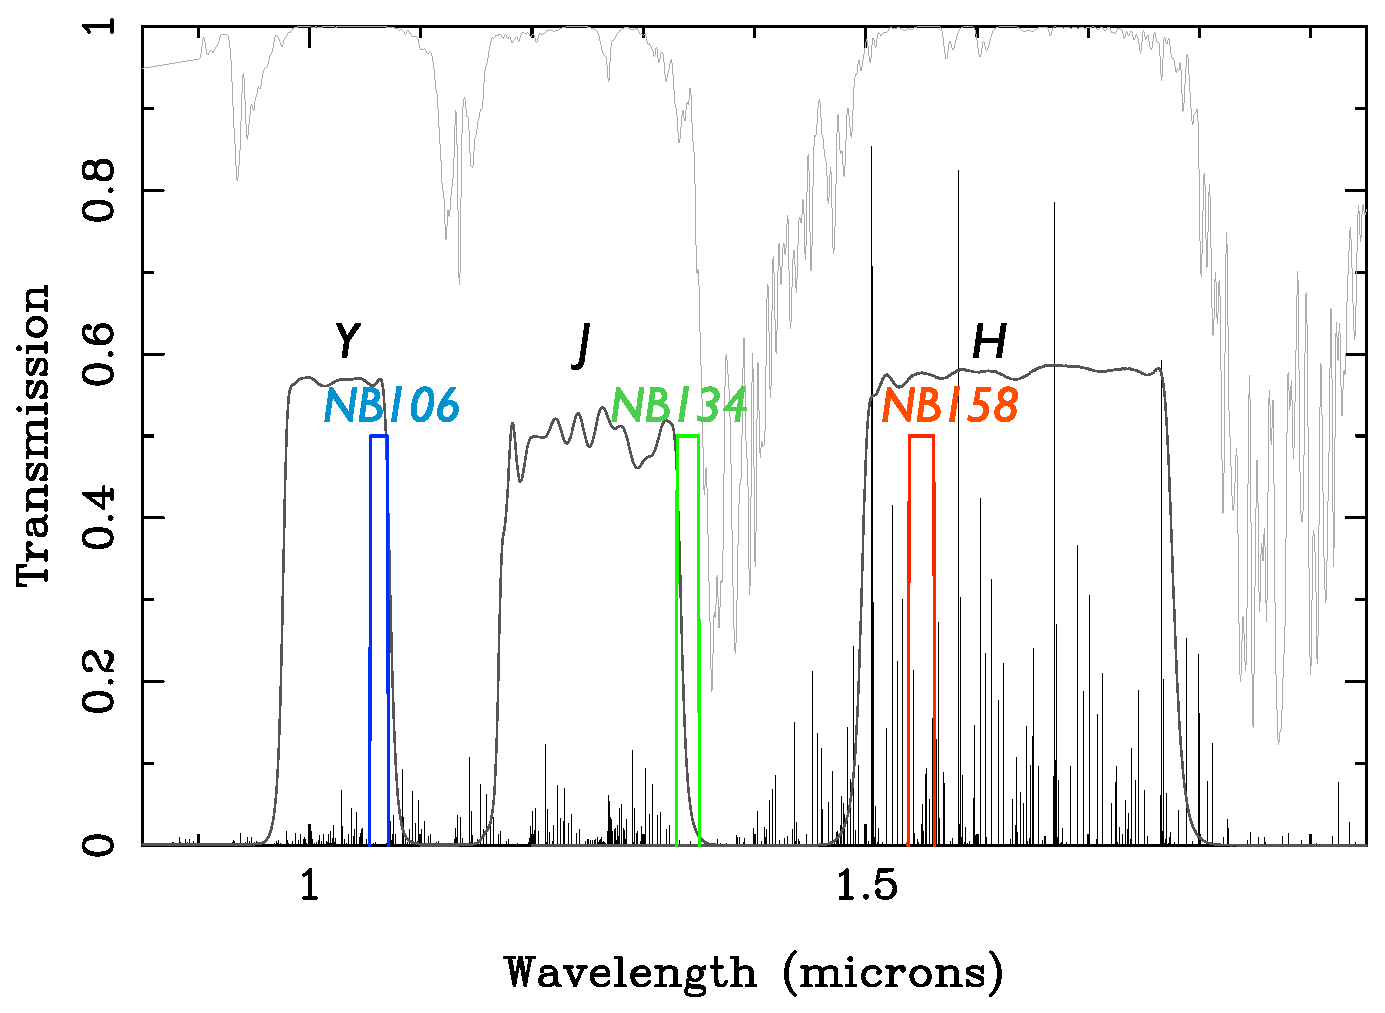
\includegraphics[width=80mm]{\thisdir figs/iwata_pg_filters_nbf01vd.eps}
}
\caption{
Transmission curves of NBFs considered. Transmission curves for $Y$,
 $J$, $H$-bands and the atomospheric transmission, and OH air glow
 strength (in arbitrary unit) are also shown.
}
\label{fig:iwata_filter_nbf}
\end{figure}

\par\noindent
[Very narrow band width filters]


\par\noindent
[What should be clarified with ULTIMATE-SUBARU.]

\subsection{Proposed Observations}

\par\noindent
[Target objects: sample selection, number of objects, number of observing
fields, sky area.]

\par\noindent
[Observing modes: imaging or spectroscopy.]

\par\noindent
[Required observing time:]

\par\noindent
[Special requirements for ULTIMATE-SUBARU other than baseline
specifications, if any.]

\subsection{Synergy and Competitions}

\subsubsection{Synergy with TMT}

\subsubsection{Competitions with other facilities}

Instruments for 8--10m class telescopes.

ELT instruments.

Space-based projects.

\bibliographystyle{apj}
\bibliography{\thisdir nbf}


%%% AO Simulation
%%%%%%%%%%%%%%%%%%%%%%%%%%%%%%%%%%%%%%%%%%%%%%%%%%%%%%%%%%%%%%%%%%%%%%%%%
% NGAO$B%o!<%/%7%g%C%WJs9p=q(B                                              %
%%%%%%%%%%%%%%%%%%%%%%%%%%%%%%%%%%%%%%%%%%%%%%%%%%%%%%%%%%%%%%%%%%%%%%%%%
%\documentclass[10pt]{jarticle}
%\usepackage{graphicx}

%\oddsidemargin   -0.25cm
%\evensidemargin  -0.25cm
%\topmargin       -0.25cm
%\textwidth        16.5cm
%\textheight       24.0cm
%\parindent        10pt

%%%%% OYA's personal new commands %%%%%
\newcommand %%%% \protect is necessary for captions %%%%%
{\supstar}{\!\!\mbox{\protect\raisebox{1.5ex}{$\star$}}}
\newcommand{\gtrsim}{\ ^{\displaystyle >}_{\displaystyle \sim}\ }
\newcommand{\lesssim}{\ ^{\displaystyle <}_{\displaystyle \sim}\ }
\newcommand{\adeg}{\hbox{$\,^{\circ}$}}
\newcommand{\arcs}{\hbox{$\,^{\prime\prime}$}}
\newcommand{\arcm}{\hbox{$\,^{\prime}$}}

\def\thisdir{simulation/glao/}

%\begin{document}

\chapter{Next-Generation AO Simulation Study
\label{chap:simulation}}

$BK\>O$G$O$9$P$kK>1s6@<!@$Be9-;kLnJd=~8w3X7O$N$?$a$N(B
$B%7%_%e%l!<%7%g%s$K4p$E$/8!F$7k2L$r$^$H$a$k!#(B
$BJd=~8w3XAuCV(B(AO: Adaptive Optics)$B$N;kLn$r9-$2$k$?$a$K$O!"(B
$BBg5$$f$i$.$N(B3$B<!859=B$$r9MN8$9$kI,MW$,$"$j!"$3$N5;=Q$r%H%b%0%i%U%#!<$H8F$V!#(B
$B%H%b%0%i%U%#!<5;=Q$r4QB,L\E*$K1~$8$F<BAu$9$k$3$K$J$k$,!"$=$NJ}<0$K$OJ#?t(B
$B$"$k(B(\ref{sec:various_ao_systems}$B@a;2>H(B)$B!#(B
$B$=$NCf$G(B
$BCOI=AXJd=~8w3X7O(B(GLAO: Ground-Layer Adaptive Optics)$B$H(B
$BB?E7BNJd=~8w3X7O(B(MOAO: Multi-Object Adaptive Optics)
$B$KBP$7$F%7%_%e%l!<%7%g%s$K$h$k8!F$$r9T$C$?!#(B

$B$9$P$kK>1s6@$K<!@$Be9-;kLn(BAO$B$rMQ$$$?@V30@~4QB,AuCV$,(B
$B3hLv$7;O$a$k:"$K$O!"8}7B(B30m$BK>1s6@$b;OF0$9$k$H4|BT$5$l$k!#(B
$B$9$P$kK>1s6@$N>-Mh7W2h$r9M$($k>e$G$O!"(B
$BL\;X$9%5%$%(%s%9$H$=$l$r<B8=$9$k5;=Q$H$$$&N>LL$K$*$$$F(B
30m$BK>1s6@$H$NAjJd@-$"$k$$$O(B30m$BK>1s6@$X$NH/E8$r0U<1$;$6$k$r$($J$$!#(B
GLAO$B$H(BMOAO$B$H$$$&(B2$B$D$N9-;kLn(BAO$B$NJ}<0$b$3$NMM$JGX7J$rF'$^$($F(B
$B%7%_%e%l!<%7%g%s$K$h$k8!F$$r?J$a$k8uJd$H$7$FA*Br$7$?!#(B
%
GLAO$B$O;kLnD>7B(B10$BJ,0J>e$H$$$&(B
$B9-;k(BAO$B$NCf$G$b:GBg$N;kLn$rC#@.$G$-$kJ}<0$G$"$k!#(B
$BJd@5@-G=$O2s@^8B3&$G$O$J$/%7!<%$%s%0$N2~A1$G$"$k$,!"(B
$B$3$N;kLn$r3h$+$9$3$H$G(B30m$BK>1s6@$HAjJdE*$J2J3XE*8&5f@.2L$,4|BT$G$-$k!#(B
$BFC$K%^%&%J!&%1%"$OBg5$$f$i$.A4BN$NCf$GCOI=AX$,@j$a$k3d9g$,Bg$-$$$3$H$,(B
$BCN$i$l$F$*$j(BGLAO$B$KE,$7$?%5%$%H$G$"$k$H8@$($k!#(B
%
MOAO$B$O9-$$;kLn$KOK$C$FF1;~$KJ#?t$NE7BN$r4QB,$9$k$3$H$G4QB,8zN($r(B
$B>e$2$k$3$H$,$G$-$kJ}<0$G$"$k!#3FE7BN$K$O2s@^8B3&$N6u4VJ,2rG=$,4|BT$G$-!"(B
$BLLJ,8w$H$NAj@-$bNI$$!#(B
MOAO$B$N<B8=$K$O?7$7$$5;=Q3+H/$,I,MW$G$"$k!#(B
$B0E$$4QB,E7BN$+$iN%$l$?J}8~$K$"$k==J,L@$k$$J#?t$NGHLL;2>H@1(B($B%,%$%I@1(B)$B$+$i!"(B
$B4QB,E7BNJ}8~$NGHLL$r?dDj$9$k%H%b%0%i%U%#!<5;=Q!"?dDj$5$l$?GHLL$r(B
$BGHLL%;%s%5(B(WFS)$B$,8+$F$$$J$$J}8~$N2DJQ7A6@(B(DM)$B$GJd@5$9$k%*!<%W%s%k!<%W@)8f5;=Q(B
$BEy$,5s$2$i$l$k!#(B
$B$9$P$kK>1s6@$K$*$$$F5;=QE*!"2J3XE*7P83$rC_@Q$7$F$$$/$3$H$G(B
30m$BK>1s6@$N<!4|4QB,AuCV$KH/E8$5$;$k$3$H$,4|BT$5$l$k!#(B

$B$3$3$G$N%7%_%e%l!<%7%g%s$O9-;kLn2=8!F$$N$?$a$G$"$k$N$G!"(B
$B$$$:$l$NJ}<0$KBP$7$F$b;kLn$r$I$3$^$G9-$/3NJ]$G$-$k$+$,(B
$B:G$b=EMW$J3NG'$9$Y$-E@$K$J$k!#(B
%
GLAO$B$N>l9g$OJd@5@-G=$,%7!<%$%s%0$K6a$$$N$G!"2s@^8B3&$r07$&0lHLE*$J(BAO$B$H$O(B
$B>u67$,0[$J$j%7!<%$%s%0$N1F6A$bBg$-$$!#(B
$B$3$N$h$&$JNN0h$G%7%_%e%l!<%7%g%s7k2L$,@5$7$$$+!"(B
$B$^$?%7!<%$%s%0%b%G%k$r$I$&Dj5A$9$k$+$KCm0U$,I,MW$G$"$k!#(B
%
MOAO$B$N>l9g$O!"8DJLE7BN$KBP$9$k9b%9%H%l!<%kHf$,L%NO$G$"$k$N$G(B
$B2s@^8B3&$N@-G=$r0];}$G$-$k;kLn$,$I$NDxEY$+!"$^$?$=$N$?$a$KI,MW$H$J$k(B
tip/tilt$B%,%$%I@1(B($BDc<!%,%$%I@1(B)$B$N?tEy$N>r7o$,CeL\$9$Y$-E@$G$"$k!#(B
%
$B$3$l$i$N9`L\$r%7%_%e%l!<%7%g%s$K$h$C$F3NG'$7$F$=$l$>$l$NJ}<0$N35MW$rGD0.$7$?(B
$B>e$G!"8!=P46EY$d%9%+%$%+%P%l!<%8$J$I$N$5$i$K>\:Y$J8!F$$X$HH/E8$5$;$F$$$/$3$H(B
$B$K$J$k!#(B

Sec.\ref{sec:gal_sim_imaging}$B$H(BSec.\ref{sec:spec_simulation}$B$G$O!"(B
GLAO$B%7%9%F%`$G$N1sJ}6d2O4QB,$,$I$N$h$&$J$b$N$K$J$k$+!"%J%A%e%i%k%7!<%$%s(B
$B%0$G$N4QB,$d2s@^8B3&$,C#@.$5$l$?>l9g$HHf3S$7$F8!F$$9$k!#(B
Sec.\ref{sec:gal_sim_imaging}$B$G$O;#A|4QB,$K$D$$$F!"(B
Sec.\ref{sec:spec_simulation}$B$G$OJ,8w4QB,$K$D$$$F$^$H$a$k!#(B



\clearpage
\begin{center}

\noindent
\Large
%%$BH/I=FbMF$N%?%$%H%k!JEvF|;H$C$?$b$N$HF10l$G$"$kI,MW$O$"$j$^$;$s!K(B
\section{Simulations of Subaru Next-Gen AO System: GLAO
\label{sec:glao_simulation}}
\vspace{0.5cm}

\noindent
\large
%%$BCx<T(B
{\bf Shin Oya$^1$}\\
$^1$ Subaru Telescope, 650 North Aohoku Place, Hilo, HI 96720, USA\\
\vspace{0.5cm}

\noindent
\normalsize
{\bf Abstract}
\end{center}
\vspace{-0.2cm}

\noindent
%abstract goes here...
$B$3$3$G$O9-;kLnJd=~8w3X7O$NCf$G$b(B10$BJ,3Q$rD6$($k:G$b9-$$;kLn$r3NJ]$G$-$k(B
$BCOI=AXJd=~8w3XAuCV(B(GLAO: Ground-Layer AO)$B$N8!F$7k2L$K4X$7$F5-=R$9$k!#(B
$B$3$NJ}<0$O>eAX$NBg5$$f$i$.$rJd@5$7$J$$$?$a!"2s@^8B3&$N@-G=$rF@$k$3$H(B
$B$G$O$J$/9-$$;kLn$K$o$?$C$F%7!<%$%s%0$r2~A1$9$k$3$H$rL\E*$H$7$F$$$k!#(B
GLAO$B$N<B8=J}K!$H$7$F$O2DJQI{6@$rF3F~$9$kJ}8~$G8!F$$r?J$a$F$$$k!#(B
$B2DJQI{6@$O(BGLAO$B0J30$K$b69;kLn$NE7BN$KBP$7$F9b$$%9%H%l!<%k$rC#@.$9$k(B
$B$3$H$,$G$-$k$N$G!"==J,L@$k$$C10l@1$KBP$9$k<+A3%,%$%I@1(B(NGS)$B4QB,!"(B
$B%3!<%s8z2L$rDc8:$9$k$?$a$NJ#?t%l!<%6!<%,%$%I@1(B(LGS)$B%H%b%0%i%U%#4QB,(B
$B$b9g$o$;8!F$$9$k$Y$-$@$H9M$($F$$$k!#(B
$B%7%_%e%l!<%7%g%s!&%3!<%I$O(BTMT$B$N(BNFIRAOS$B$N$?$a$K3+H/$5$l$?(BMAOS$B$r;HMQ$7$?!#(B



%%$BK\J83+;O!J>ON)$F$O<+M3!K(B

%%% 20130311 ommited by Iwata

%%%%%%%%%%%%%%%%%%%%%%%%%%%%%%%%%%%%%%%%%%%%%%%%%%%%%%%%%%%%%%%%%%%%%%%%%
%% NGAO$B%o!<%/%7%g%C%WJs9p=q%F%s%W%l!<%H(B
%%%%%%%%%%%%%%%%%%%%%%%%%%%%%%%%%%%%%%%%
%%
%% [AO$B$HAuCV$N;EMM(B] $B3F<+MW5a$9$k(BAO$B$dAuCV$N;EMM$r%F%s%W%l!<%H$K$"$kI=$K5-F~!#(B
%%
%% [$B;29MJ88%(B] $BI,$:L@5-$9$k$3$H!#?^$N0zMQ85$bL@5-$9$k$3$H!#(B
%%
%% [$BJ,NL(B] $B4pD49V1i(B(20$BJ,0J>e(B)$B$O(B4$B%Z!<%80J>e!"0lHL9V1i(B(15$BJ,(B)$B$O(B2$B%Z!<%80J>e!#(B
%%
%% [$BDy@Z(B] $B869FDy$a@Z$j(B 2012$BG/(B1$B7nKv(B
%%
%%%%%%%%%%%%%%%%%%%%%%%%%%%%%%%%%%%%%%%%%%%%%%%%%%%%%%%%%%%%%%%%%%%%%%%%%

%\documentclass[10pt]{jarticle}
%\usepackage{graphicx}

%\oddsidemargin   -0.25cm
%\evensidemargin  -0.25cm
%\topmargin       -0.25cm
%\textwidth        16.5cm
%\textheight       24.0cm
%\parindent        10pt

%\def\gsim{\mathrel{\raise0.35ex\hbox{$\scriptstyle >$}\kern-0.6em % Greater/squiggles
%\lower0.40ex\hbox{{$\scriptstyle \sim$}}}}
%\def\lsim{\mathrel{\raise0.35ex\hbox{$\scriptstyle <$}\kern-0.6em % Less than/squiggles 
%\lower0.40ex\hbox{{$\scriptstyle \sim$}}}}

%\begin{document}

\def\thisdir{simulation/moao/}

\begin{center}

\noindent
\Large
\section{Simulations of Subaru Next-Gen AO System: MOAO
\label{sec:moao_simulation}}
\vspace{0.5cm}

\noindent
\large
%%$BCx<T!JNc!K(B
{\bf Masayuki Akiyama$^1$}\\
$^1$ Astronomical Institute, Tohoku University, 3-6 Aramaki, Aoba-ku, Sendai, Japan
\vspace{0.5cm}

\noindent
\normalsize
{\bf Abstract}
\end{center}
\vspace{-0.2cm}

\noindent
$B$3$3$G$O$9$P$kK>1s6@$K$*$$$F(B6$B8D$N%l!<%6!<%,%$%I@1$rMQ$$$F(B
$BB?E7BNJd=~8w3X(B(MOAO)$B$r9T$C$?>l9g$KM=A[$5$l$k@-G=$r8!F$$7$?(B
$B7k2L$r$^$H$a$k!#FC$K!"(BMOAO$B$rMQ$$$k$3$H$GCO>eAXJd=~8w3X(B(GLAO)
$B$h$j$b9b$$Jd=~@-G=$r9-$$NN0h$NB?E7BN$K$D$$$F<B8=$9$k$3$H$r(B
$BL\;X$9!#$=$N$?$a(BGLAO$B$h$j$b9b$$Jd=~@-G=$r0];}$7$D$D!"$I$NDxEY(B
$B$^$G%?!<%2%C%HNN0h$r9-$2$i$l$k$N$+$rI>2A$9$k$3$H$K=EE@$r(B
$BCV$/!#(BMOAO$B$N>l9g$K$O;kLn$NCf$rO"B3E*$KJd@5$9$k$3$H$O$;$:!"(B
$BFCDj$N%?!<%2%C%H$NJ}8~$N$_$NJd@5$r9T$C$F$$$k$3$H$KCm0U$,(B
$BI,MW$G$"$k!#$=$N$?$a0J2<$G$O$3$N%?!<%2%C%H$rA*Br$9$kNN0h$N(B
$B$3$H$r%?!<%2%C%HNN0h$H8F$V!#(B6$B8D$N%l!<%6!<%,%$%I@1$rMQ$$$?(B
$B>l9g!"H>7B(B$3^{\prime}$$BDxEY$N%?!<%2%C%HNN0h$K$D$$$F$O(BGLAO
$B$h$j$b9b$$Jd=~@-G=$,4|BT$5$l$k$,!"$=$l$h$j$b%l!<%6!<%,%$%I@1$N(B
$B4V3V$r9-$2$F%?!<%2%C%HNN0h$r9-$2$k$H;kLn$N$[$H$s$I$NNN0h(B
$B$G(BGLAO$B$K6a$$Jd=~@-G=$7$+F@$i$l$:!"(BMOAO$B$N%a%j%C%H$,(B
$B@8$+$;$J$/$J$k$3$H$,$o$+$C$?!#$^$?<+A3%,%$%I@1$N4V3V$,3+$/$K$D$l(B
$B$F(B Tip-Tilt $B$NGHLL8m:9$,5^7c$KBg$-$/$J$k$3$H$b$o$+$C$?!#(B
Tip-Tilt $B%,%$%I@1$KMQ$$$k$3$H$N$G$-$k<+A3%,%$%I@1$NL@$k$5(B
$B$r9M$($k$H6d6KJ}8~$K$*$$$F$OJ#?t$N<+A3%,%$%I@1$r%?!<%2%C%H(B
$BNN0h$KMQ0U=PMh$k3NN($O$+$J$jDc$/!"(BTip-Tilt $B$NGHLL;D:9$,(B
$B@-G=$r%j%_%C%H$9$k!#(B


%%$BK\J83+;O!J>ON)$F$O<+M3!K(B

%%% 20130311 ommitted by Iwata

% galaxy simulation: imaging
% galaxy simulation: spectroscopy

%%% System Design
%\documentclass[10pt]{jarticle}
%\usepackage{graphicx}
%\usepackage{url}

%\oddsidemargin   -0.25cm
%\evensidemargin  -0.25cm
%\topmargin       -0.25cm
%\textwidth        16.5cm
%\textheight       24.0cm
%\parindent        10pt

%\def\gsim{\mathrel{\raise0.35ex\hbox{$\scriptstyle >$}\kern-0.6em % Greater/squiggles
%\lower0.40ex\hbox{{$\scriptstyle \sim$}}}}
%\def\lsim{\mathrel{\raise0.35ex\hbox{$\scriptstyle <$}\kern-0.6em % Less than/squiggles 
%\lower0.40ex\hbox{{$\scriptstyle \sim$}}}}

\def\thisdir{development/design/}

%\begin{document}

\chapter{System Study for Subaru Next-Generation AO
\label{chap:system_design}}

\section{Comparisons of Candidate AO Systems for Subaru Telescope
 Next-Generation AO
\label{sec:various_ao_systems}}

%%% 20130311 ommited by Iwata

\section{Overview of the System}

%%% 20130311 ommited by Iwata.
%%% Need to include overview of NIR instrument(s) as well?

$B8=;~E@$G5DO@$,?J$a$i$l$F$$$k<!@$Be(BAO$B$*$h$S@V30@~AuCV$N(B
$B4pK\;EMM$rI=(B\ref{tab:spec}$B$K<($7$?!#$3$N;EMM$O:#8e$N>\:Y$J(B
$B8!F$$K$h$C$F$OBgI}$KJQ99$5$l$k2DG=@-$,$"$k!#(B
\begin{table}[t]
\begin{center}
\begin{tabular}{|l|l|l|l|l|}
\hline
 Item & Specification \\
 \hline
 $B4QB,GHD90h(B & 0.9--2.5 $\mu$m ($B%5%$%(%s%9(BWS$B$+$i$NMW5a$O(B0.6--5$\mu$m\\
 $B4QB,%b!<%I(B & $B;#A|!"J,8w!JLLJ,8w$r9MN8$9$k!K(B\\
 $B4QB,;kLn(B & $\phi$ 15$BJ,3Q!J(B20$BJ,3QL\I8!K(B\\
 $B>GE@0LCV(B & $B%+%;%0%l%s>GE@(B \\
 \hline
 $B%,%$%I@1(B & 4 LGS$B!"(BNGS$B!J(B2$\sim$4$B8D$+!)!K(B\\
 $B%,%$%I@1$NA*BrHO0O(B & LGS$B$O4QB,;kLn$NC<!"(BNGS$B$O4QB,;kLnFb(B \\
 $BGHLL%;%s%5!<(B & $B%,%$%I@1$K$=$l$>$l(B1$B$D$:$D(B (Guide star oriented)\\
 $BGHLL%;%s%5!<%?%$%W(B & $B%7%c%C%/%O%k%H%^%s7?!J%T%i%_%C%I7?$bMW8!F$!K(B \\ 
 $BGHLL%;%s%5!<AG;R?t(B & 100$BDxEY$+$=$l0J>e(B ($B9b%9%H%l!<%k$J$i(B1000$BAG;RDxEY$b(B) \\
 $BGHLL%;%s%5!<%5%s%W%j%s%0<~GH?t(B & 500Hz$B0J>e!J(BGLAO$B$O(B100Hz$B$G$b2D!K(B \\
 $B2DJQ7A6@(B & $BI{6@$r2DJQ7A6@2=(B \\
 $B2DJQ7A6@AG;R?t(B & 500$\sim$1000$BDxEY(B \\
 $BGHLL@)8f%b!<%I(B & GLAO (LTAO$B!"(BExAO$B$J$I$X$N@ZBXBP1~$,I,MW$+!)(B)\\
 \hline
\end{tabular}
\caption{$B<!@$Be(BAO$B$*$h$SAuCV$N4pK\;EMM0F(B}
\label{tab:spec}
\end{center}
\end{table}

\section{Technical Challenges}

$B>e=R$7$?(BTomography AO$B$K6&DL$9$k5;=QE*$J2]Bj$O!"(B
$B%l!<%6!<5;=Q$*$h$SJ#?t%l!<%6!<%,%$%I@1$N@=:n5;=Q!"(B
$BBg5$$f$i$.$N9b$5J}8~$N(Btomography$B?dDj5;=Q!"(B
$B2DJQI{6@!"@)8f7W;;5!$J$I$,$"$k!#(B
$B$?$@$7!"@$3&$ND,N.$H$7$F(Btomography AO$B$O@9$s$K(B
$B%7%9%F%`8!F$!"5;=Q8!F$$,?J$a$i$l$F$*$j!"(B
$B5;=QE*$J2]Bj$O$+$J$j9nI~$5$l$D$D$"$k$N$,8=>u$G$"$k!#(B

$B=i4|$N%l!<%6!<%,%$%I@1$O?'AG%l!<%6!<$,<gBN$G$"$C$?!#(B
$B$3$l$O%l!<%6!<G^<A$,1UBN$G$"$j!"0BDj@-!"J]<i@-$K(B
$BBg$-$JO+NO$,I,MW$G$"$k!#$^$??'AG$NNt2=$K$h$k=PNODc2<$,(B
$BHr$1$i$l$J$$!#<!$KH>F3BN%l!<%6!<$H%l!<%6!<7k>=$N(B
$B5;=QH/E8$,$"$j!"8GBN%l!<%6!<$,BfF,$7$F$/$k!#(B
$B:#$G$O%J%H%j%&%`AX$rNe5/$9$k$?$a$NOB<~GHH/@8$rMQ$$$?(B
$BA48GBN%l!<%6!<$,5;=QE*$K@.=O$7$F$-$?!#(B
Gemini$B$N(BMCAO$B$G$O=PNO(B50W$B$N%l!<%6!<$r(B5$B$D$KJ,3d$7$F!"(B
5$B8D$N%J%H%j%&%`%l!<%6!<%,%$%I@1$N:n@.$K@.8y$7$F$$$k!#(B
$B0lJ}!"%U%!%$%P!<%l!<%6!<5;=Q$rMQ$$$?%3%s%Q%/%H$+$D(B
$B0BDj$7$?%l!<%6!<$N3+H/$,(BESO$B$rCf?4$K?J$a$i$l!"(B
$B%I%$%D$N(BTOPTICA$B<R$H%+%J%@$N(BMPB$B<R$N6&F1$G(B
$BO"B3GH(B20W$B$N%l!<%6!<$,@=IJ2=$5$l$?!#(B
$B$3$N%l!<%6!<$OB>$N(B8m$B%/%i%9$N<!@$Be(BAO$B$*$h$S(B
ELT$BMQ(BAO$B$N%l!<%6!<%,%$%I@1MQ8w8;8uJd$H$7$FBg$-$J(B
$B4|BT$,4s$;$i$l$F$$$k!#2f!9$b$9$G$K(BMPB$B<R$H(B
$BHkL)J];}7@Ls$rDy7k$7!"5;=Q>pJs$N8r49!"(B
$B4pK\;EMM$N8!F$=`Hw$r?J$a$F$$$k!#(B
$B$^$?!"%l%$%j!<;6Mp$rMxMQ$7$?%l!<%6!<%,%$%I@1$b(B
WHT$B!"(BMMT$B$J$I$GCOF;$K;n83$,B3$1$i$l$F$$$k!#(B
8m$B%/%i%9$N(Bsingle conjugate $B%l!<%6!<%,%$%I@1(BAO$B$,(B
$B0BDj$7$F1?MQ$5$l$F$*$j!"%l!<%6!<%,%$%I@1$K(B
$B4X$9$k4pAC5;=Q!"1?MQ5;=Q$O$*$*$$$K?JJb$7$?!#(B
$B%l!<%6!<%7%9%F%`$K$D$$$FI=(B\ref{tab:Laser}$B$K$^$H$a$?!#(B

\begin{table}[t]
\begin{center}
\begin{tabular}{|l|l|l|l|l|l|l|l|}
\hline
 %$BK>1s6@(B & Subaru & Keck I & Keck II & Gemini N & VLT  & Gemini S & LBT \\
% \hline
%$B%l!<%6!<%,%$%I@1(B & Na$BAX(B & Na$BAX(B & Na$BAX(B & Na$BAX(B. & Na$BAX(B  & Na$BAX(B & $B%l%$%j!<;6Mp(B \\
%$B%l!<%6!<%?%$%W(B & $BOB<~GH(B & $BOB<~GH(B & $B?'AG(B & $BOB<~GH(B. & $B?'AG(B->$B%U%!%$%P!<(B  & $BOB<~GH(B & $BA48GBN%0%j!<%s(B \\
%$B%l!<%6!<G^<A(B & $B8GBN7k>=(B & $B8GBN7k>=(B & $B?'AGM-5!1UBN(B & $B8GBN7k>=(B. & $B?'AGM-5!1UBN(B->$B8w%U%!%$%P!<(B  & $B8GBN7k>=(B & $B8GBN7k>=(B \\
%$B=PNO(B & $\sim$6W & $\sim$40W & $\sim$15W & $\sim$15W & $\sim$10W->$\sim$25W & $\sim$10W / beacon & $\sim$18W / beacon \\
%$B%l!<%6!<H/?67ABV(B & 143MHz & 75MHz & 13kHz or 26kHz & 75MHz & $BO"B3GH(B & 75MHz & 10kHz \\
$B%,%$%I@1%?%$%W(B & \multicolumn{3}{|c|}{$B%J%H%j%&%`AX(BLGS} &  \multicolumn{1}{|c|}{$B%l%$%j!<(BLGS} \\
\hline
$B%l!<%6!<%?%$%W(B & $B?'AG(B & $BA48GBNOB<~GH(B & $B8w%U%!%$%P!<%l!<%6!<(B & $BA48GBN!!(B\\
\hline
$B%l!<%6!<G^<A(B & $B1UBNM-5!MOG^(B & $B8GBN7k>=(B & $B8w%U%!%$%P!<(B& $B8GBN7k>=(B \\
\hline
$BK>1s6@(B & Keck II & Subaru, Keck I & VLT$B!J<!@$Be!K(B & LBT \\
             & VLT & Gemini N\&S &       &  (Na-LGS$B$b7W2hCf(B) \\
\hline
$B=PNO(B & 15W(Keck II) & 6W(Subaru) & 25W(VLT$B<!@$Be(B) & 18W$\times$3 (LBT) \\
    &    &  40W(Keck I) & & \\
    &  10W(VLT) & 15W(GeminiN) & &  \\
    &    &  10W$\times$5 (GeminiS) & & \\
\hline
$BH/?67ABV(B & 26kHz(Keck II) & 143MHz(Subaru) & $BO"B3GH(B(VLT$B<!@$Be(B) & 10kHz(LBT) \\
  & $BO"B3GH(B(VLT) & 75MHz(Keck I) & & \\
  &   & 75MHz(Gemini N\&S) & & \\
\hline
\end{tabular}
\caption{$B%l!<%6!<%,%$%I@1MQ%l!<%6!<%7%9%F%`$NHf3S(B}
\label{tab:Laser}
\end{center}
\end{table}


$B:GBg3QEY$G$b(B10$BJ,3Q$H$$$&69$$HO0O$N8w8;$rMQ$$$F!"(B
$BESCf$K$"$kBg5$$f$i$.$N(B3$B<!85J,I[$r?dDj$9$k(B
tomography$B?dDj5;=Q$O!"0lHL$N(B3$B<!85(Btomography$B$H$O(B
$B$+$J$j0[$J$kMWAG$r4^$s$G$$$k!#$7$+$7!"B?$/$N(B
AO tomography$B%"%k%4%j%:%`$,Ds>'$5$l!"7W;;5!(B
$B%7%_%e%l!<%7%g%s!"%F%9%H%Y%C%I$K$h$k<B83$,(B
$B?J$a$i$l$F$-$?!#>\:Y$J8!F$$*$h$S%7%9%F%`$KFC2=$7$?(B
$B8!F$$O$^$@I,MW$G$"$k$,!"4pACE*$J(BAO tomography$B$N(B
$B8&5f$O==J,$J$5$l$F$-$F$$$k!#$9$P$k<!@$Be(BAO$B8!F$(B
$B%o!<%-%s%0%0%k!<%W$O!":#8e>\:Y8!F$$rB3$1$F$$$/M=Dj$G$"$k!#(B

$BFC$K(BGLAO$B$O2DJQI{6@$,=EMW$J%3%s%]!<%M%s%H$H$J$k!#(B
$BF|K\$G$O$^$@2DJQI{6@$N8!F$$O?J$a$i$l$F$$$J$$$,!"(B
$B%"%j%>%J$N(BMMT$B!"(BLBT$B$G$O$9$G$K2DJQI{6@$,Ek:\$5$l!"(B
$BL@$k$$%,%$%I@1$G$h$$Jd@5@-G=$rC#@.$7$F$$$k!#(B
$B$^$?%A%j$N(BVLT$B$N$?$a$N2DJQI{6@$,@=:nCf$G$"$k!#(B
$B$3$l$i$N2DJQI{6@$r@=:n$7$?$N$O%$%?%j%"$N(BMicrogate$B<R$G$"$k!#(B
$B2f!9%o!<%-%s%0%0%k!<%W$O$9$G$K(BMicrogate$B<R$H%3%s%?%/%H$r$H$j!"(B
$B$9$P$kK>1s6@MQ$N2DJQI{6@$N35G08!F$$N=`Hw$r?J$a$F$$$k!#(B

$BJ#?t$N%,%$%I@1!"J#?t$"$k$$$OB?AG;R$N2DJQ7A6@$r@)8f$9$k$?$a$N(B
$B7W;;5!$KMW5a$5$l$k@-G=$OHs>o$K9b$$!#2f!9%o!<%-%s%0%0%k!<%W$O!"(B
$B$^$@@)8f7W;;5!$N8!F$$r;O$a$F$$$J$$$,!"(BTMT$BMQ$N%U%!!<%9%H%i%$%H(BAO
$B$G$"$k(BNFIRAOS$B$N@)8f7W;;5!8!F$$,==J,;29M$K$J$k$H9M$($F$$$k!#(B

\section{Interfaces with the Subaru Telescope -- 20130311Iwata: to be ommitted?}

$B$9$P$kK>1s6@<!@$Be(BAO$B$NBh0l8uJd$G$"$k(BGLAO$B$K$D$$$F!"(B
$BK>1s6@$H$N%$%s%?!<%U%'!<%9$r9M;!$7$?!#(B
GLAO$B$N:GBg$NFCD'$O!"2DJQI{6@$rMQ$$$F$$$k$3$H$G!"(B
$BH?<MLL$,>/$J$/8zN($,9b$$$3$H$,$"$2$i$l$k!#(B
$B=>$C$F!"4QB,AuCV$O%+%;%0%l%s>GE@$K@_CV$9$k$N$,$h$$!#(B
$B$^$?!"(BGLAO$B$G$O(B10$BJ,3Q$rD6$($k;kLn$,L%NO$H$J$C$F$$$k!#(B
$B8=:_;H$o$l$F$$$k%+%;%0%l%s>GE@$N2D;kMQBg5$J,;6Jd@58w3X7O$O(B
$B$=$3$^$G$N;kLn$r3NJ]$G$-$F$$$J$$!#(BGLAO$B$H6a@V30@~4QB,AuCV$N(B
$BAH$_9g$o$;$N$H$-$OBg5$J,;6Jd@58w3X7O$O<h$j30$9I,MW$,$"$k!#(B

$B%+%;%0%l%s>GE@$N4QB,AuCV$N8!F$$b=EMW$G$"$k!#(B
GLAO$B$N9-;kLn$r@8$+$96a@V30@~;#A|J,8wAuCV$r8!F$$9$k>e$G!"(B
$BK>1s6@$N8w3X<}:9!"AuCV$N%5%$%:!"=ENL!"@_7W@=B$2DG=$J8w3X7O$N@_7W(B
$B$J$I$,=EMW$J%U%!%/%?!<$H$J$k!#(B

$B2DJQI{6@$O$9$P$kK>1s6@$N%H%C%W%f%K%C%H$K@\B3$5$l$k!#(B
$B$9$P$kK>1s6@$O<g>GE@It$K9-;kLn%+%a%i$J$I$r(B
$BEk:\$9$k$?$a!"%H%C%W%f%K%C%H8r495!$N=ENL@)8B$,(B
3t$B$G$"$k!#8=:_@=:nCf$N(BVLT$BMQ2DJQI{6@$NAm=ENL$O(B1500kg
$BDxEY$J$N$G7ZNL2=$NEXNO$OITMW$G$"$k!#(B
$B8=:_;HMQCf$N@V30I{6@$OD>7B$,(B1265mm$B$G$"$j!"(B
VLT$B$N2DJQI{6@D>7B$h$j$b<c43Bg$-$$!#(B
$B%+%;%0%l%s>GE@$N(BF$BCM$NJQ99$b9MN8$7$?2DJQI{6@$N;EMM:vDj$r(B
$B:#8e?J$a$F$$$/$3$H$K$J$k!#(B
$B%H%C%W%f%K%C%H$K$*$1$kEENO6!5k!"@)8f@~!"%M%C%H%o!<%/!"Nd5Q?e(B
$B$J$I$N4pK\E*$J%$%s%U%i!"%H%C%W%f%K%C%H$H$N%$%s%?!<%U%'!<%9!"(B
$B$J$I$N8!F$$b=EMW2]Bj$G$"$k!#(B

\section{Subaru GLAO System Structure}


%%% 20130311 ommitted by Iwata

%%% 20130311 additions by Iwata
\section{Components of GLAO: Adaptive Secondary Mirror}

\section{Components of GLAO: Wavefront Sensing System}

\section{Components of GLAO: Laser System}

\section{Components of GLAO: RTC}

%%% 20130311 additions by Iwata
\section{Telescope Modifications}

\subsection{Top Unit}

\subsection{Cassegrain Focus}

\subsection{Other Areas?}



\section{Operations of GLAO}

$B$9$P$kK>1s6@$O<g>GE@4QB,AuCV$,$"$k$?$a!"2DJQI{6@$r>o@_$9$k$3$H$O(B
$B1?MQ>e$G$-$J$$!#$=$N$?$a!"2DJQI{6@$O%H%C%W%f%K%C%H8r49AuCV$r(B
$BMQ$$$FCeC&$9$kI,MW$,$"$k!#$=$N$?$a$N%$%s%?!<%U%'!<%9;EMM$r(B
$B3NDj$7$J$1$l$P$J$i$J$$!#$^$?2DJQI{6@$NIT;HMQ;~$NJ]4I>l=j$N3NJ]$H(B
$B$=$N%$%s%?!<%U%'!<%9$H%$%s%U%i$N;EMM$K$D$$$F$b7h$a$kI,MW$,$"$k!#(B
$B$^$?!"8r49;~$N4D6->r7o!"?6F0>r7o!"6@$NJ];}$"$k$$$O0BA4$J>uBV4IM}$K(B
$B$D$$$F$b8!F$$rMW$9$k!#(B

$B0lJ}!"$9$P$kK>1s6@$NI{6@$OFLLL$G$"$k!#FLLL$N2DJQI{6@$N%-%c%j%V%l!<%7%g%s(B
$BJ}K!$K$D$$$F$b8!F$$,I,MW$@!#$^$?!"2DJQI{6@$N:F>xCe$NI,MW@-!"Dj4|E*$J(B
$BJ]<i9`L\$J$I$b=i4|8!F$$NCJ3,$G5DO@$7$F$*$/$Y$-$G$"$m$&!#(B

$B%l!<%6!<<M=P%7%9%F%`$O!"K>1s6@$N%;%s%?!<%;%/%7%g%s$K>o@_$9$k$3$H$r(B
$B8!F$Cf$G$"$k!#CeC&$NI,MW@-$O$J$$$,!"%l!<%6!<$NJ]<i!"ItIJ$N8r49!"(B
$B7PG/JQ2=$X$NBP1~!"0BA44IM}$r4^$a$?%l!<%6!<1?MQBN@)$OI,?\$H$J$k!#(B

$BGHLL%;%s%5!<$O%+%;%0%l%s>GE@>eIt$N%+%;%0%l%s%U%i%s%8$H8F$P$l$kCf$K(B
$B@_CV$5$l$k!#$3$NItJ,$O%"%/%;%9$,BgJQFq$7$/!"AuCV$N8N>c!"2~=$$,(B
$BFq$7$$!#$=$N$?$a$N7xO4!"J]<iITMW$NGHLL%;%s%5!<%7%9%F%`8!F$$OBg@Z$G$"$m$&!#(B

\section{Perspective of Future Development}

GLAO$B%7%9%F%`$O<g$H$7$F2DJQI{6@!"%+%;%0%l%s%U%i%s%8$NGHLL%;%s%5!<!"%l!<%6!<(B
$B<M=P7O!"4QB,AuCV$H$$$&9=@.$+$i$J$k!#$3$N%3%s%]!<%M%s%H$OB>$N(BAO$B%7%9%F%`$K(B
$B$H$C$F$b=EMW$J9=@.MWAG$G$"$k!#(B

$B2DJQI{6@$NAG;R?t$O(B1000$BDxEY$H$J$k8+9~$_$G$"$k!#$=$N$?$a!"L@$k$$<+A3%,%$%I@1MQ$N(B
$BGHLL%;%s%5!<$r4QB,AuCVB&$KMQ0U$9$k$H!"%+%;%0%l%s!"%J%9%_%9$N$$$:$l$N>GE@$K$b(B
Extreme AO$BAuCV$,$G$-$k!#$b$A$m$s!"8=B8$"$k$$$O7W2hCf$N9b%3%s%H%i%9%H4QB,AuCV$K$b(B
$B1~MQ$,$G$-$k$G$"$m$&!#2DJQI{6@$OCf4V@V30@~$NAuCV$NGX7J8w$r2!$5$($kMxE@$H$b$J$k!#(B

$B$^$?!"J#?t%l!<%6!<<M=P7O$O(BMOAO$B$KMxMQ$G$-!"2DJQI{6@$O(BMOAO$B$N(Bwoofer$B$H$7$F;HMQ$7!"(B
$B4QB,AuCVB&$K(BMOAO$B$N(Btweeter$B2DJQ7A6@$r$b$?$;$k$3$H$G!"8zN($NNI$$AuCV$,9M0F$G$-$k$G$"$m$&!#(B

$B$3$N$h$&$K(BGLAO$B%7%9%F%`$OK>1s6@5!G=$N%]%F%s%7%c%k$NDl>e$2$r$9$k$b$N$G$"$k!#(B

%\end{document}


%%% Telescope
%%% 20130312 iwata skelton
\def\thisdir{development/telescope/}

\chapter{Interface with Subaru Telescope
\label{chap:tel}}

%%% 20130311 additions by Iwata
\section{Telescope Modifications: Top Unit}

\section{Telescope Modifications: Cassegrain Focus}

\section{Telescope Control Software}

\section{Other Areas?}




%%% Instruments
\def\thisdir{instrument/}

\chapter{Instruments for Subaru Next-Generation AO
\label{chap:inst}}


\section{Requirements on Instrument from Scientific Objectives}

Here we re-summarize the requirements from key science cases on
instrument specifications.

\begin{itemize}
 \item Field of view
 \item Pixel scale
 \item Requirements on broad-band filters (numbers, wavelength coverages)
 \item Requirements on narrow-band filters (numbers, spectral resolution,
      wavelength uniformity, wavelength coverages)
 \item Spectroscopy: Spectral resolution 
 \item Requirements on multi-object spectrograph mode
\end{itemize}

In this chapter we summarize the studies we have made so far on
instruments for ULTIMATE-SUBARU.

\def\thisdir{instrument/optics/}

\begin{center}
\section{Studies of the Optics for the Wide-Field Near-IR Imager and
 Multi-object Spectrograph
\label{sec:inst_optics}}
\vspace{0.5cm}

\noindent
\large
%% authors
{\bf T. Yamamuro$^{1}$, K. Motohara$^{2}$, I. Iwata$^{3}$ and Subaru
Telescope Next-Gen AO Instrument sub-working group}\\
$^1$ Optocraft
$^2$ Institute of Astronomy, University of Tokyo
$^3$ Subaru Telescope, National Astronomical Observatory of Japan
\vspace{0.5cm}

\end{center}

Here we summarize results of studies made by Dr. Yamamuro (Optcraft).
Document Number: CP0046--11--RP001 (w/o FoV split), CP0046--12--RP001 (w
FoV split).

\subsection{Optical Design without FoV Split}

First we studied how wide field of view can be achieved at the
Cassegrain focus of Subaru Telescope with the following conditions:

\begin{itemize}
 \item Single set of optics can be used (i.e., no FoV split is
       considered).
 \item We consider a near-infrared camera and spectrograph. Wavelength
       range is from 0.8$\mu$m to 2.5$\mu$m. The optics will be cooled
       down to about 100K.
 \item The target image quality is to achieve FWHM $<0.15''$ over the
       entire FoV in all of $J$, $H$, $K$-bands.
 \item The focal plane of the instrument should be flat so that we can
       achieve the above image quality by using science detectors with
       flat pixel arrays.
 \item The use of Teledyne H4RG (15$\mu$m pixel size) is assumed.
 \item The sizes of optical components should be feasibile; for example,
       the maximum size of components made of CaF$_2$ and BaF$_2$ should
       be less than 40cm.
\end{itemize}

We examined the two cases on the telescope parameters; (A) the case we
use the existing optical parameters of Subaru Telescope and (B) the case
with new parameters for the secondary mirror and also that the shape of 
primary mirror can be adjusted within the range of the stroke which the
existing mirror actuators are achievable.

Also, we should consider the necessity of field flatner for the
telescope focus. In order to achieve multi-object spectroscopy (MOS), we
need to insert a mask with slitlets at the telescope focus. Since the
Cassegrain focal plane has a curvature, in order to enable the use of
flat MOS mask, we need to insert field flatning lens(es). For the case
A, we show both the case with and without field flatner.

\subsubsection{A. Cases in which Subaru Telescope optical parameters are
   not changed}

Here we show the simplest case where there is no change in the telescope 
parameters and no field flatner is included.
Fig.\ref{fig:optcraft_fig01} is the optical layout. It consists of nine
collimator lenses and seven camera lenses. Lense materials are CaF$_2$, 
BaF$_2$, Fused silica, and ZnSe.The last lens of the camera section is
aspherical. 

\begin{figure}[!ht]
\centerline{
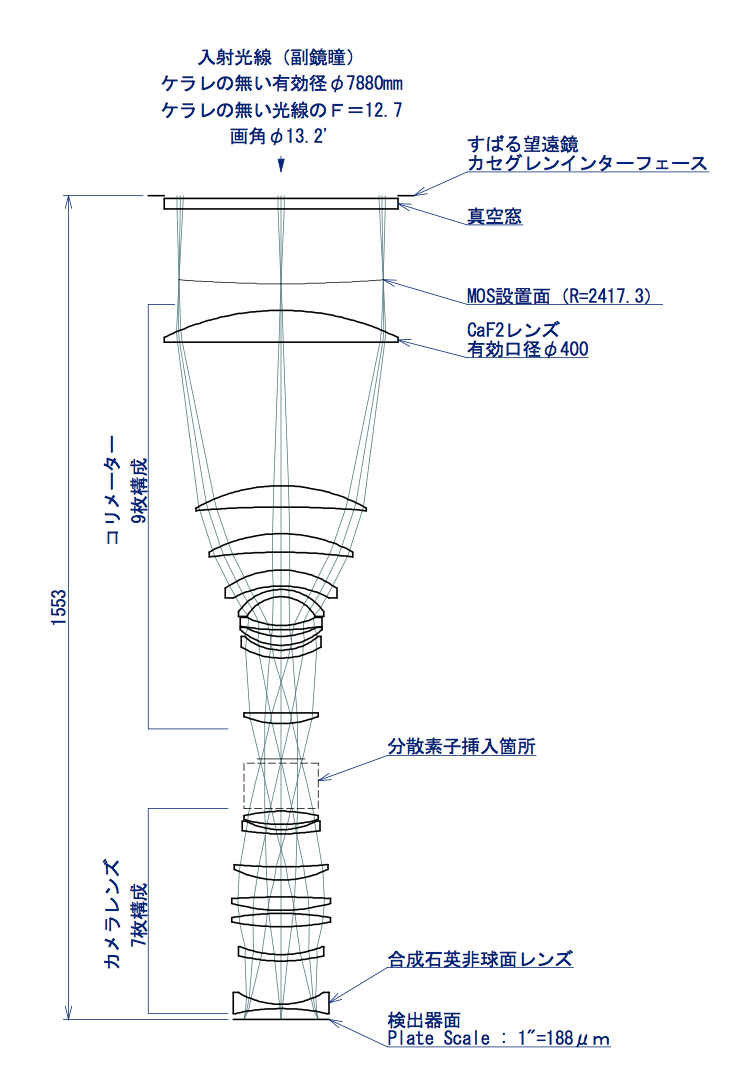
\includegraphics[width=120mm]{\thisdir figs/optcraft_fig01.eps}
}
\caption{Optical layout for Case A: no change in the telescope
 parameters. The case without field flatner.
}
\label{fig:optcraft_fig01}
\end{figure}

The field of view is determined so that the size of effective beam for
the largest lens is within $\phi$400mm, and in this solution it is 
$\phi 13.2'$. The effective diameter of the primary mirror is 
$\phi 7.88$m to achieve the above FoV at the secondary mirror pupil and
to block the light outside of the primary mirror (physical size 
$\phi$8.2m). Since this layout does not include field flatner, the
telescope focal plane has a curvature, and there is astigmatism.

The spot diagram at the position of the MOS mask (with a radius of
curvature of 2417.3mm) is shown in
Fig.~\ref{fig:optcraft_fig02}(left). The degradation of the image toward
the edge of FoV ($\sim 0.2''$ at the edge) is due to astigmatism. 
In this case the slit width at the edge should be adjusted to this image
quality. 
Fig.~\ref{fig:optcraft_fig02}(right) shows the size of distortion at the
position of the MOS mask.

\begin{figure}[!ht]
\centerline{
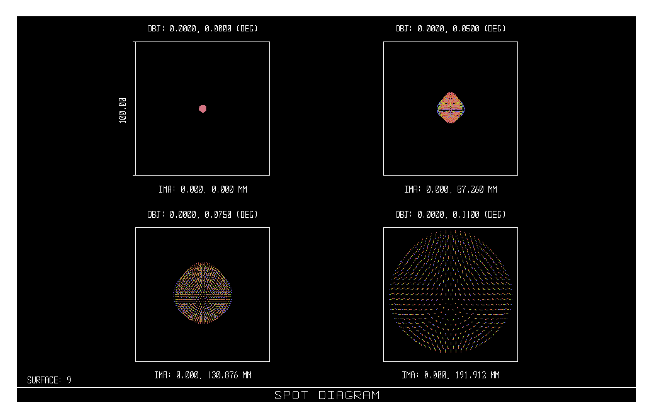
\includegraphics[width=100mm]{\thisdir figs/optcraft_fig02.eps}
 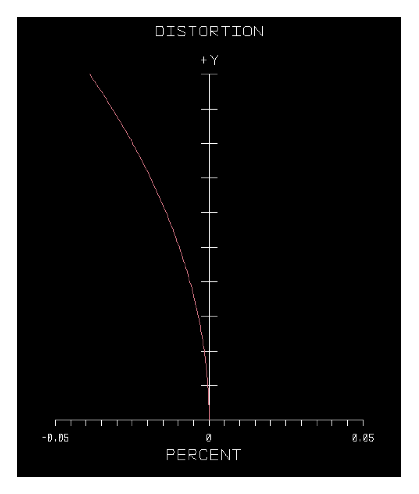
\includegraphics[width=60mm]{\thisdir figs/optcraft_fig03.eps}
}
\caption{(Left) Spot diagram at the position of the MOS mask with a
 curvature radius of 2417.3mm for a configuration shown in 
Fig.\ref{fig:optcraft_fig01}. Spot diagrams with wavelengths from
 0.8$\mu$m to 2.5$\mu$m are shown altogether, as wavelength dependence
 is small. (Right) distortion at the
 position of the MOS mask. The value is $-0.04$\% at the edge.
}
\label{fig:optcraft_fig02}
\end{figure}

The spot diagram and distortion at the position of the detectors are
shown in Fig. \ref{fig:optcraft_fig04}. All FWHM values are smaller than
the target FWHM (0.15$''$) except the case with 0.8$\mu$m
at the edge ($6.6'$) in which the FWHM is slightly larger than
0.15$''$. However, the distortion is large; at the edge it is 
$-6.3$\%.

\begin{figure}[!ht]
\centerline{
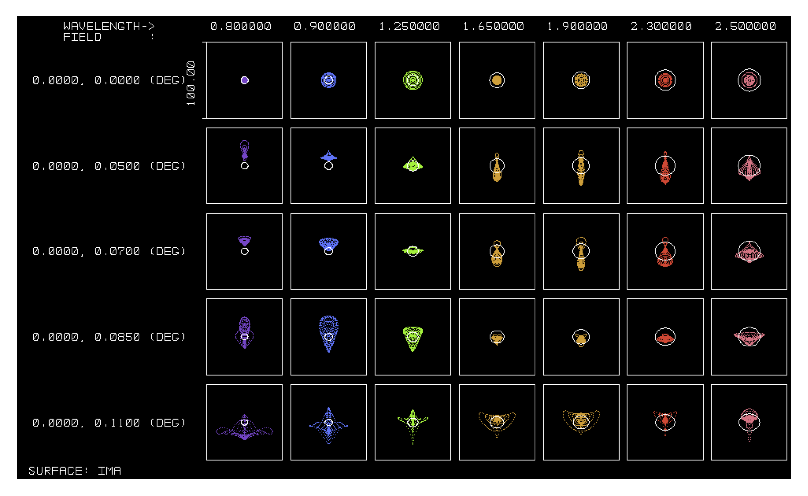
\includegraphics[width=120mm]{\thisdir figs/optcraft_fig04.eps}
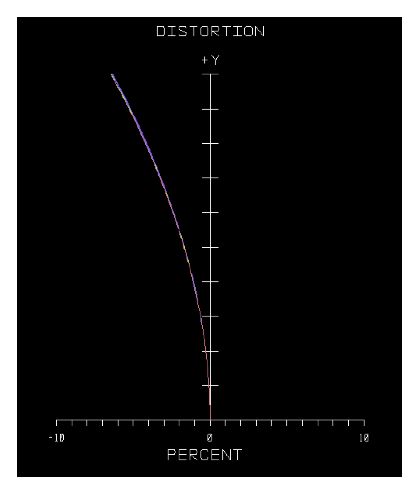
\includegraphics[width=60mm]{\thisdir figs/optcraft_fig05.eps}
}
\caption{(Left) Spot diagram at the position of the detectors for a
 configuration shown in Fig.\ref{fig:optcraft_fig01}.
Five positions from 0$'$ (center) to 6.6$'$ (edge) are shown along the
 vertical axis, and the cases with wavelengths from 0.8$\mu$m to
 2.5$\mu$m are plotted along the horizontal axis. 
The box size is 100$\mu$m which corresponds to 0.53$''$.
(Right) Distortion at the position of the detectors.
}
\label{fig:optcraft_fig04}
\end{figure}


We also evaluated the performance in spectroscopy. As a preliminary
analysis, here we only examined the image quality in spectroscopy in the
range 0.8--2.5$\mu$m without order-sorting.
Fig.~\ref{fig:optcraft_fig06} shows the positions of images in
spectroscopy as a function of wavelength.
Here we assume a fused silica grism with 160 grooves/mm, blaze angle 
34$\circ$\footnote{In section ** we examine more details of various
grisms}.
Fig.~\ref{fig:optcraft_fig07} is the spot diagram. Image qualities at
the shorter and longer wavelength edges and at the edge of FoV is not
good; in 2.5$\mu$m and at $6.6'$ from the center the RMS spot diameter
is $0.22''$. However, it is $0.17''$ at $5.5'$ from the center, and
at the other positions the image quality meets the goal.

\begin{figure}[!ht]
\centerline{
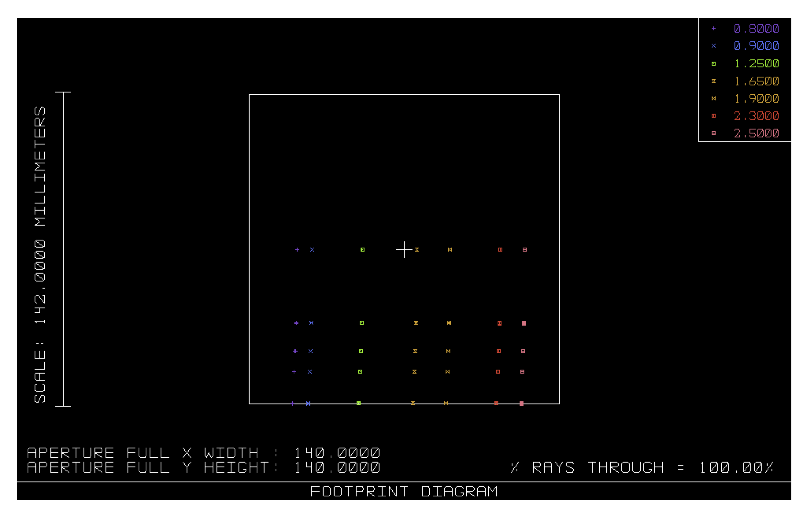
\includegraphics[width=120mm]{\thisdir figs/optcraft_fig06.eps}
}
\caption{Spectroscopic image positions for a configuration shown in Fig.~\ref{fig:optcraft_fig01}.
}
\label{fig:optcraft_fig06}
\end{figure}

\begin{figure}[!ht]
\centerline{
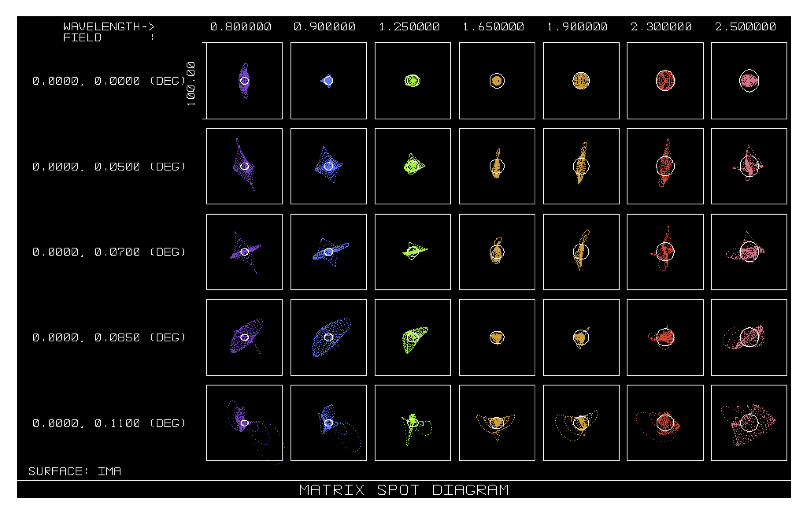
\includegraphics[width=120mm]{\thisdir figs/optcraft_fig07.eps}
}
\caption{Spot diagram for spectroscopy with a configuration shown in
 Fig.~\ref{fig:optcraft_fig01}.}
\label{fig:optcraft_fig07}
\end{figure}

Next we examined the case where there is no change in the telescope
parameters again, and a field flatner which consists of two lenses. 
Fig.~\ref{fig:optcraft_fig08} shows the optical layout of the case.

\begin{figure}[!ht]
\centerline{
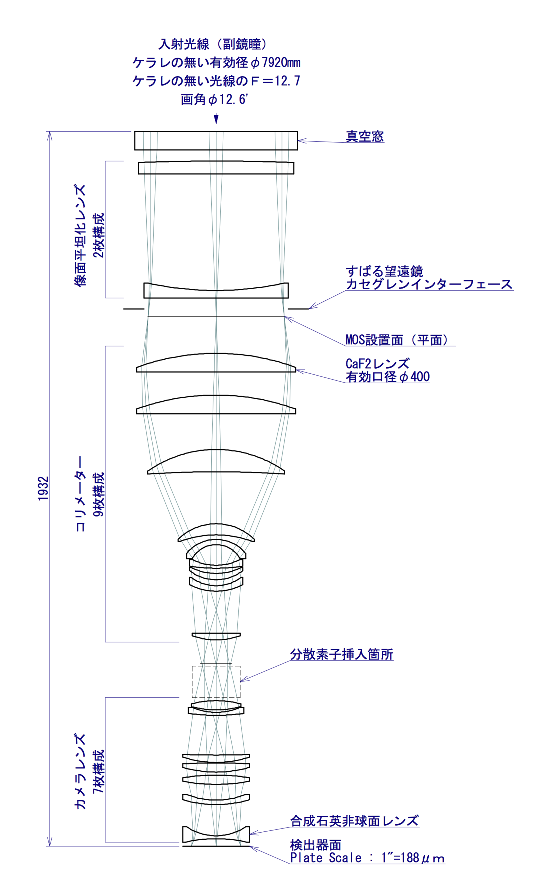
\includegraphics[width=120mm]{\thisdir figs/optcraft_fig08.eps}
}
\caption{Optical layout for Case A: no change in the telescope
 parameters. The case with field flatner.
}
\label{fig:optcraft_fig08}
\end{figure}

The optical design was made so that the effective diameter of the
largest lens is no larger than $\phi$400mm, as it is in the case without
the flatner. The field of view is $\phi 12.6'$, which is slightly
smaller than the case without the flatner, because the field flatner
acts like a concave lens and we need collimator lenses larger than the
flatner. The effective diameter of the primary mirror to block the light
outside of the primary mirror is $\phi$7.92m.
In addition to make the telescope focal plane flat, the addition of the
flatner enables a correction of astigmatism. As shown in 
Fig.~\ref{fig:optcraft_fig09}, the image quality is good at the flat MOS
mask, and there is no chromatic abberation.
We should note that there is distortion, which amounts +0.73\% at the
edge of the FoV.

\begin{figure}[!ht]
\centerline{
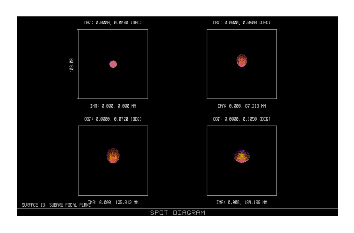
\includegraphics[width=100mm]{\thisdir figs/optcraft_fig09.eps}
 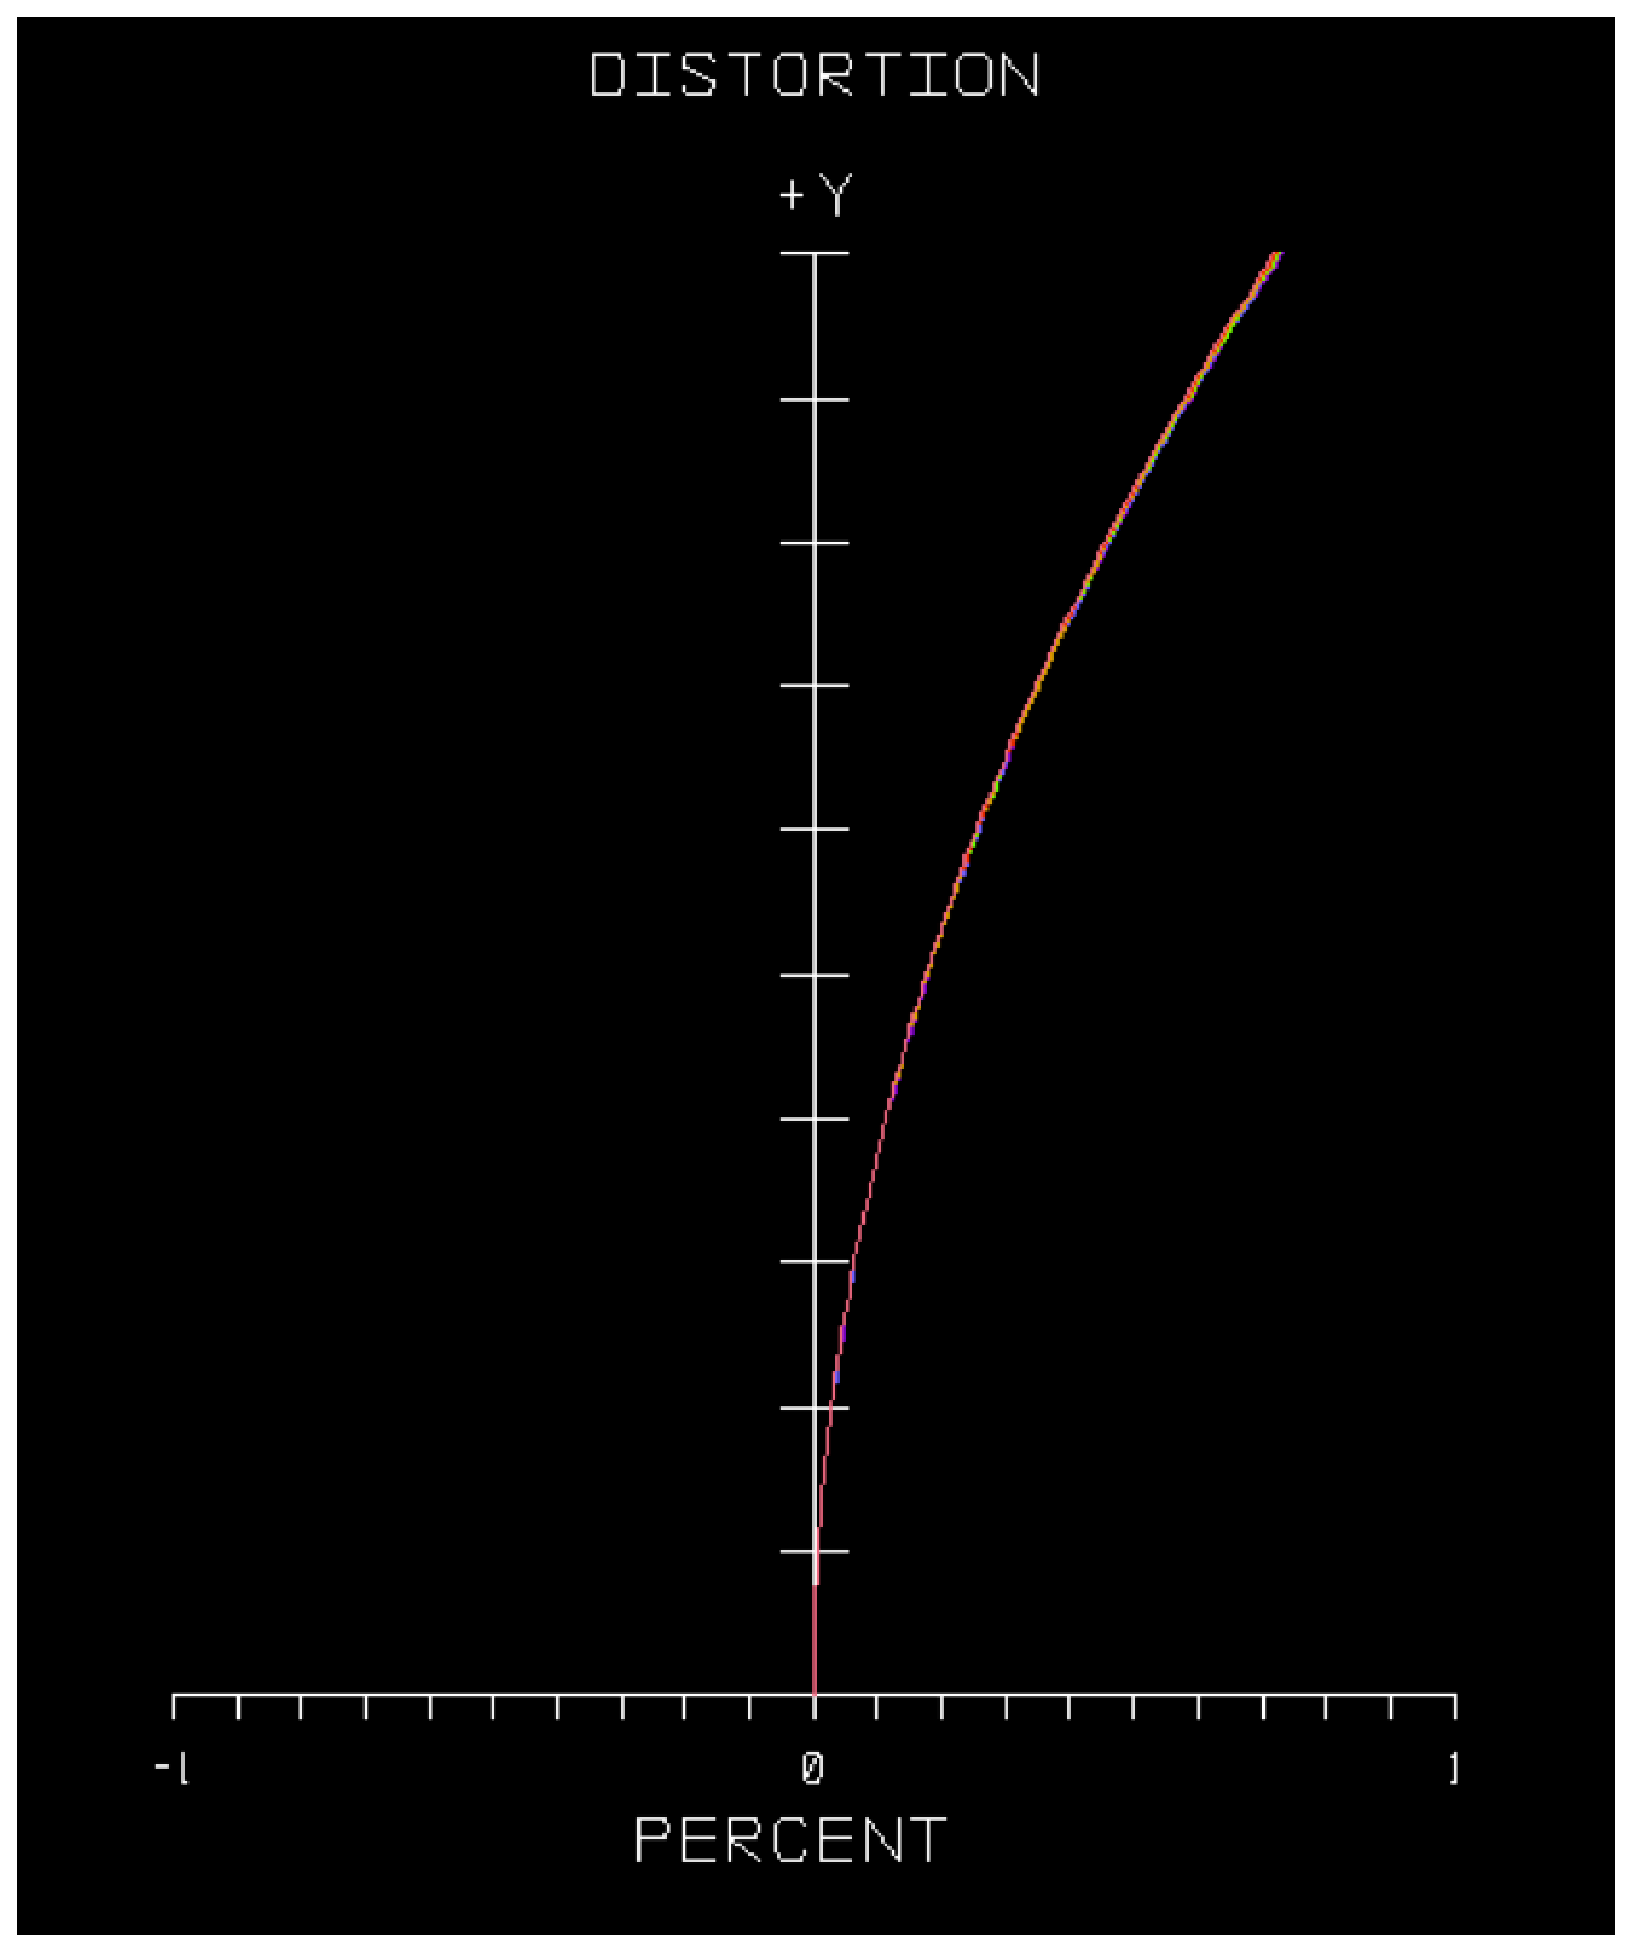
\includegraphics[width=60mm]{\thisdir figs/optcraft_fig10.eps}
}
\caption{(Left) Spot diagram at the MOS mask plate.
(Right) distortion at the MOS mask plate.
}
\label{fig:optcraft_fig09}
\end{figure}

For the image quality at the position of the detectors, similar to the
case without the flatner, in the most of the FoV and for the most of the
wavelength range the image quality satisfies the goal (FWHM smaller than
approx. $0.15''$), while in a few cases (such at the FoV edge ($6.3'$
from the center) and with 0.8$\mu$m) the image quality is slightly worse
than the goal. Distortion is large; it is $-5.2$\% at the edge of FoV.
Performance in the spectroscopy is also similar to the case without the
flatner, and in most cases the qulality satisfies the goal.
We should note that with the field flatner the optical layout is not
telecentric, and the plate scale should be changed if there is a focus
offset.  So the focusing is more important in this case.




\subsubsection{B. Cases in which Subaru Telescope optical parameters are
   changed}

Next we examined the case in which Subaru Telescope's optical parameters
are changed. In order to make the telescope's F number smaller, the
primary mirror's aspheric parameters should be negative. The actuator
storoke for the primary mirror is guaranteed up to 12$\mu$m. We assume
the conic parameters so that displacement at the edge of the primary
mirror is 12$\mu$m, and set F number to be 9.8.

The parameters of the secondary mirror is determined as it is optimal
for this Cassegrain wide-field instrument, and it is independent from
the existing secondary mirrors of Subaru Telescope.
It is a bipolar mirror with a diameter of $\phi$1544mm. The radius of
curvature is 7233.308mm and the conic constant is $-2.35464$.
The field of view is determined by the effective maximum size of the
lens ($\phi$400mm), and it is $\phi16.2'$.
Thanks to the smaller F number, the field of view is 28\% larger than
the case without changing the telescope parameters. The effective
diameter of the primary mirror to avoid the beam outside of the
secondary pupil and primary mirror ($\phi$8.2m) is $\phi$7.93m.

\begin{figure}[!ht]
\centerline{
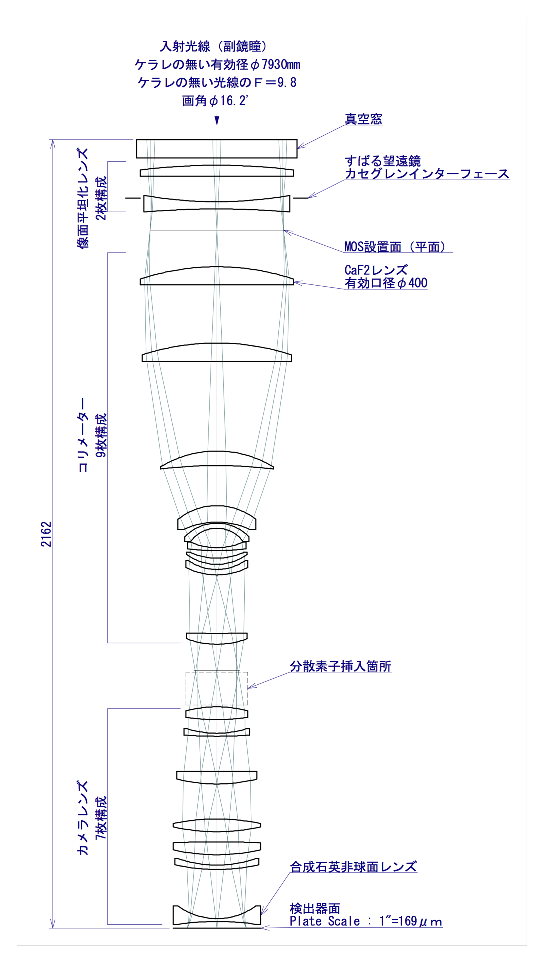
\includegraphics[width=120mm]{\thisdir figs/optcraft_fig15.eps}
}
\caption{The optical layout of the case B: Subaru Telescope
 optical parameters are modified. A field flatner is included in this
 design. 
}
\label{fig:optcraft_fig15}
\end{figure}

In this design a set of lenses as a field flatner is included. 
The spot diagram at the flat MOS mask position is presented in 
Fig. \ref{fig:optcraft_fig16}.
Although small coma aberration is present, its effect is small. There is
no chromatic aberration, overall image quality is good, although there
is distortion aberration at the edge of the FoV.

\begin{figure}[!ht]
\centerline{
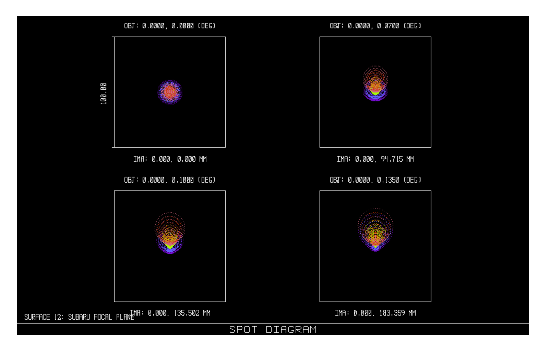
\includegraphics[width=100mm]{\thisdir figs/optcraft_fig16.eps}
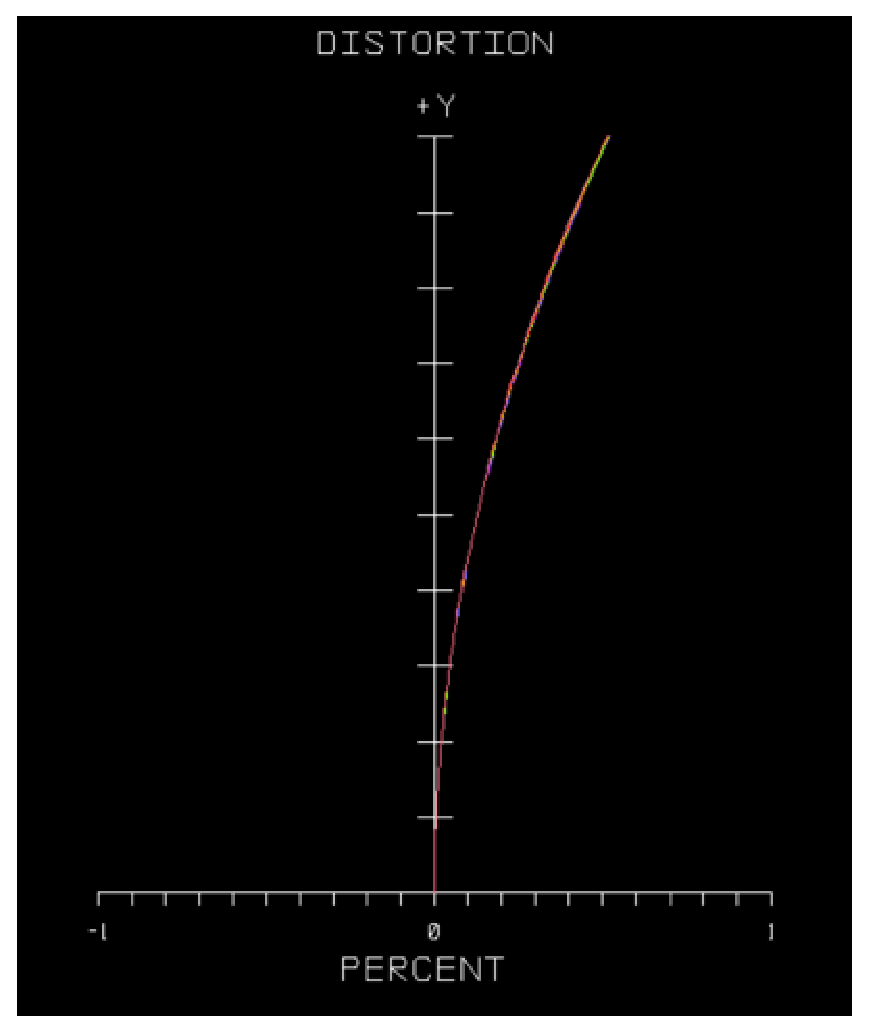
\includegraphics[width=60mm]{\thisdir figs/optcraft_fig17.eps}
}
\caption{(Left) Spot diagram at the MOS mask position.
(Right) distortion aberration at the MOS mask position.
}
\label{fig:optcraft_fig16}
\end{figure}

The configuration of optics after MOS position is similar to the case
without change of the telescope parameters: collimator with nine lenses
and camera with seven lenses. The focal plane is flat. The optical
layout in shown in Fig.\ref{fig:optcraft_fig15}.

In Fig. \ref{fig:optcraft_fig18} we show the spot diagram and distortion
aberration at the position of detectors.
Image quality at outskirt of the FoV ($>6'$) in a short wavelength
(0.8--0.9$\mu$m) degrades by $\sim0.2''$. Otherwise image quality
satisfies the goal (FWHM$\sim 0.15''$).
The maximum distortion aberration at the edge of FoV is $-1.24$\%, which
is smaller than the cases without changes in telescope parameters.

\begin{figure}[!ht]
\centerline{
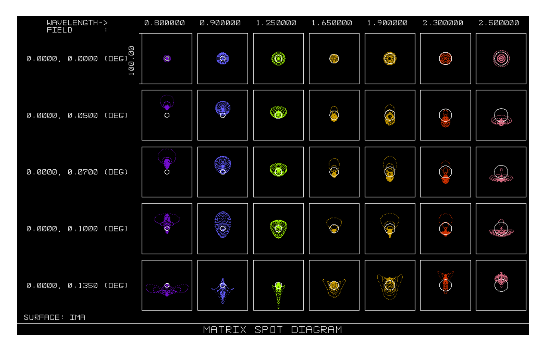
\includegraphics[width=120mm]{\thisdir figs/optcraft_fig18.eps}
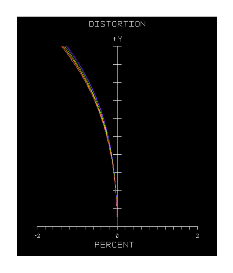
\includegraphics[width=60mm]{\thisdir figs/optcraft_fig19.eps}
}
\caption{(Left) Spot diagram at the positions of the detectors.
Images with five positions within the FoV (vertical) and seven
 wavelengths from 0.8$\mu$m to 2.5$\mu$m (horizontal) are plotted.
The box size is 100$\mu$m, which corresponds to $0.59''$.
The RMS spot diameters are $0.2''$ (at $8.1'$, $0.8\mu$m), 
$0.16''$ (at $6'$, $0.8\mu$m), $0.19''$ (at $6'$, $0.9\mu$m), and for
 other positions and wavelength the spot diameters are within $0.15''$.
(Right) Distortion aberration. It reaches to $-1.24$\% at the edge of
 the FoV.
}
\label{fig:optcraft_fig18}
\end{figure}

Performance in spectroscopy mode is examined and is reported in 
Fig.~\ref{fig:optcraft_fig20}. Here a grism made of fused silica, 160
lines/mm, blaze angle 35$^\circ$ is assumed, and the sizes of spectra on
the detector is presented.

In regards to the image quality, as shown in
Fig.~\ref{fig:optcraft_fig21}, in some cases at the edge of FoV or
shortest/longest wavelengths the RMS spot diameter becomes as large as 
$0.23''$. Otherwise the image quality satisfies the goal, especially
within $6'$ from the center of FoV.

\begin{figure}[!ht]
\centerline{
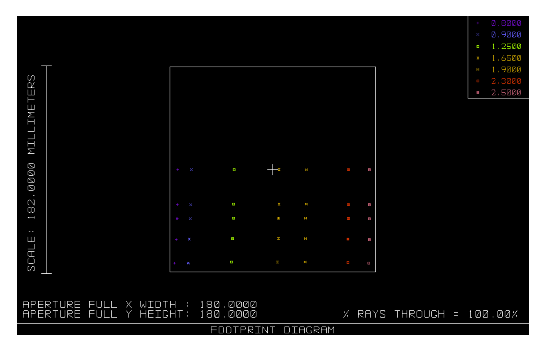
\includegraphics[width=120mm]{\thisdir figs/optcraft_fig20.eps}
}
\caption{
Spectroscopic image positions for a configuration shown in
 Fig.~\ref{fig:optcraft_fig15}. The box size is 180mm. We assume to use
 a grism made of fused silica with 160 lines/mm, and blaze angle
 35$^\circ$.
}
\label{fig:optcraft_fig20}
\end{figure}

\begin{figure}[!ht]
\centerline{
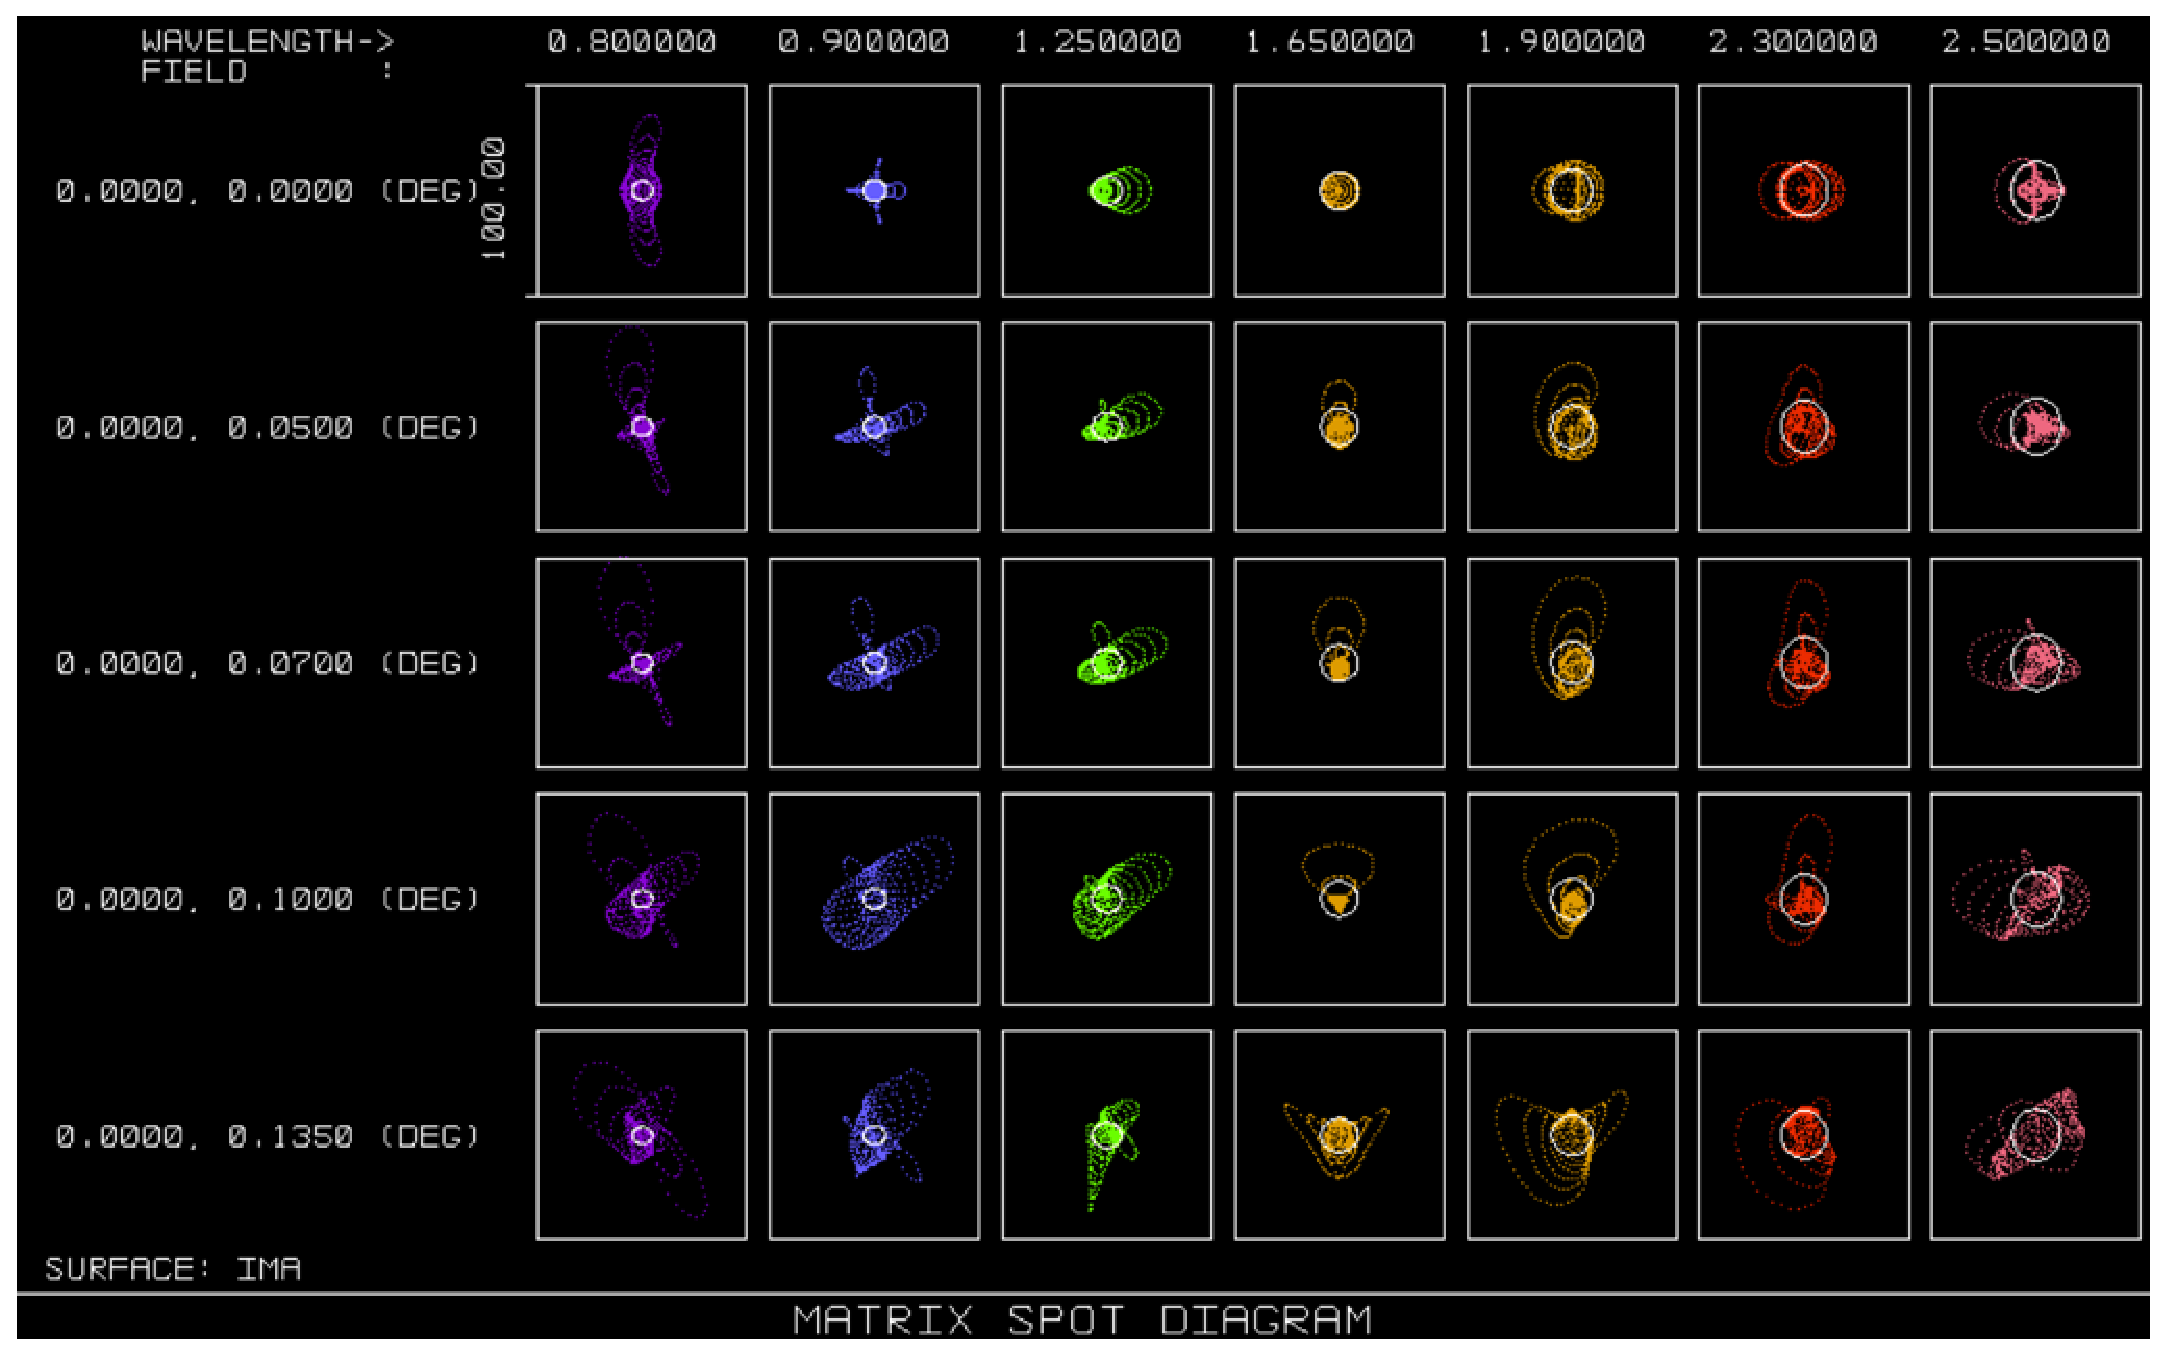
\includegraphics[width=120mm]{\thisdir figs/optcraft_fig21.eps}
}
\caption{Spot diagram for Case B, spectroscopy mode.
In shorter wavelength the performance is somewhat worse than the goal;
 at 0.8$\mu$m RMS spot diameters are in general 0.17--0.18$''$, and 
 0.2$''$ at 0.9$\mu$m. In longer wavelength spot diameter becomes larger
 at positions with distance from the center larger than $6'$ with
 $\lambda = 2.3-2.5\mu$m. Otherwise the image quality satisfies the goal
 ($0.15''$).
}
\label{fig:optcraft_fig21}
\end{figure}



\subsection{Optical Design with FoV Split}

\subsubsection{Case A: secondary mirror parameter is the same as
   existing one}

\subsubsection{Case B: secondary mirror parameter is modified}



\def\thisdir{instrument/mechanics/}

\begin{center}
\section{Studies of the Mechanics for the Wide-Field Near-IR Instrument
\label{sec:inst_mechanics}}
\vspace{0.5cm}

\noindent
\large
%% Authors
{\bf TBD}\\
\vspace{0.5cm}

\end{center}



%%% Development Plan
\def\thisdir{plan}

\chapter{Development Plan
\label{chap:dev_plan}}

\section{Overview of the Development Plan}

$B$9$P$kK>1s6@$OF|K\$NE7J83X%3%_%e%K%F%#$NK>1s6@$G$"$k!#(B
$B=>$C$F!"$9$P$kK>1s6@<!@$Be(BAO$B$O$=$NE7J83X%3%_%e%K%F%#$N%K!<%:(B
$B$r==J,H?1G$5$;$F@_7W!"@=:n$9$k$Y$-$G$"$k!#(B
$B0lJ}!"$9$P$kK>1s6@$O<+A32J3X8&5f5!9=9qN)E7J8Bf$,1?1D$7$F$$$k!#(B
$B$=$N$?$a!"9qN)E7J8BfA4BN$N>-Mh7W2h$N0lIt$H$7$F$9$P$k<!@$Be(B
AO$B$O?d?J$5$l$J$1$l$P$J$i$J$$!#(B

2012$BG/8=:_!"$9$P$kK>1s6@$G$OD69-;kLn<g>GE@%+%a%i$NN)$A>e$2$,(B
$B?J$a$i$l$F$$$k!#$^$?!"?tJ*2J3X8&5f5!9=$rCf?4$H$7$F!"D69-;kLn(B
$B<g>GE@%U%!%$%P!<J,8w4o7W2h$,;O$a$i$l$?!#0lJ}!"9qN)E7J8Bf$O(B
$BD6Bg7?8w3X@V30@~K>1s6@!"(BTMT$B7W2h$N%Q!<%H%J!<$H$7$F;22h$7$F$$$k!#(B
$B$3$N$h$&$J>u67$NCf$G!"$9$P$kK>1s6@$N<!@$Be@V30@~AuCV$HJ?9T$7$F(B
$B<!@$Be(BAO$B7W2h$,N)$A>e$2$D$D$"$k!#$3$NAuCV7W2h$OF|K\$N8w@V30E7J83X(B
$B%3%_%e%K%F%#$rBeI=$9$k(BSAC$B$N>-MhAuCV9=A[$KDs0F$5$l$F$$$?$b$N$G$"$k!#(B

% comment-out by iwata on 2012/05/07
%$B%7!<%$%s%0%j%_%C%H$N9-;kLnAuCV72(B
%S-CAM,FMOS,MOIRCS (HSC,PFS)
%$B%G!<%?!"%5%$%(%s%9$N7P83$NC_@Q(B
%$B<g>GE@AuCV$r;Y$($k9=B$(B

%$BB>K>1s6@$H$N4X78(B
%8m$B5iK>1s6@$O2?$+$7$i$N9-;kLn(BAO$B7W2h$,$"$k(B
%30m$B5iK>1s6@;~Be$NAjJd@-(B
%    (8m$B$N=88wNO$H3QEYJ,2rG=$@$1$G$O6%AhNO$,$J$/$J$k(B)

$B$9$P$kK>1s6@$N:GBg$NFCD'$O!"<g>GE@D69-;kLnAuCV$G$"$k(BSupreme Cam$B!"(B
FMOS$B!"$=$7$F(B2012$BG/Cf$K%3%_%C%7%g%K%s%0$,3+;O$9$k(BHyper Supreme Cam$B!"(B
$B7W2h$,?J9TCf$N(BPFS$B$G$"$k!#$5$i$K%+%;%0%l%s>GE@$K$O(BFOCAS$B!"(BMOIRCS$B$,(B
$B$"$k!#$3$l$i$N4QB,AuCV$r$D$+$C$?7P83$*$h$S%G!<%?$NC_@Q$O5.=E$G$"$k!#(B
$B$^$?!"$9$P$kK>1s6@$O!"B>$N(B8m$B%/%i%9K>1s6@$H$O0c$$!"<g>GE@AuCV$rEk:\(B
$B$G$-$k$h$&$J7xO4$+$D0BDj$7$?K>1s6@9=B$$r;}$C$F$$$k!#(B2020$BG/Be$K$O!"(B
30m$B%/%i%9K>1s6@$,BfF,$7;O$a$k$?$a!"(B8m$B%/%i%9K>1s6@$N=88wNO$H3QEYJ,2rG=(B
$B$@$1$G$O6%Ah$7$F$$$/$3$H$,$G$-$J$$!#$3$l$i$NE@$r9MN8$7!"(B
$B<!@$Be(BAO$B$*$h$S@V30@~AuCV8!F$%0%k!<%W$O9-;kLn$rBh0l$N%-!<%o!<%I$H$7$F$-$?!#(B
$B$=$N7k2L!"Bh0l8uJd$H$7$F(BGLAO$B$H9-;kLn6a@V30@~;#A|!&(B($BLL(B)$BJ,8wAuCV$r(B
$B<!@$BeAuCV$H$7$F5s$2$?!#(BTMT$B$NsUL@4|!"(BJWST$BEy$N1'ChK>1s6@;~Be$K$*$$$F!"(B
$B$3$NAuCVDs0F$O==J,$J6%AhNO$HO"7HNO$,$"$j!"B>$NCO>e(B8$\sim$10m$B%/%i%9(B
$BK>1s6@$K$*$1$k<!@$BeJd=~8w3X$*$h$S@V30@~AuCV$H$N6%Ah$H=;$_J,$1$,(B
$B2DG=$G$"$k$H4|BT$5$l$k!#(B

$BK\8!F$Js9p=q$NBh(B\ref{chap:science}$B>O$G$O!"9-$$4QE@$+$i$_$?<!@$Be(BAO
$B$*$h$S@V30@~AuCV$K$h$k!":#8eH/E8$9$k$G$"$m$&%5%$%(%s%9%1!<%9$NDs0F$r(B
$B=8$a$?!#<!@$Be(BAO$B$*$h$SAuCV;EMM$KBP$9$kMW5a$N=EMW$J;qNA$G$"$k!#(B
$B0z$-B3$-!"MM!9$J%5%$%(%s%9%1!<%9$K$D$$$F5DO@$r?<$a$F$$$/$Y$-$G$"$k!#(B

$B0lJ}!"(BAO$B$N@-G=%7%_%e%l!<%7%g%s$HL\I8@-G=!"AuCV$N35G08!F$$r?J$a!"(B
$BHs>o$K=iJbE*$JAuCV;EMM$*$h$SAuCV3+H/7W2h$r9M0F$7$D$D$"$k!#(B

$BK\>O$O$=$N7W2h$N35MW$K$D$$$F=R$Y$F$$$/!#(B

\section{Development Organization}

\subsection{International Partnership}


\section{Budget}

\subsection{Fund-Raising Plan}


\section{Development Schedule}



\end{document}


%%%% structure in '2012 Japanese edition of Study Report'

%%% Science
\chapter{Science with ULTIMATE-SUBARU 
\label{chap:science}}

In this chapter we introduce science cases proposed to be carried out
with Subaru Telescope Next-Generation AO (ngAO) and clarify
specifications ngAO and associated new instruments should satisfy.

The GLAO system we are studying have following features (see
Chapter~\ref{chap:system_design} for details):

\begin{itemize}
\item Wide-field seeing improvement by correcting WFE caused by ground
      layer of the Earth's atmosphere. Seeing improvement will provide
      not only better angular resolution, but also the significant
      improvement of sensitivity especially for point-like sources. On
      the other hand, the WFE correction (and subsequently angular
      resolution) for individual sources are not as good as classical AO
      systems (such as AO188 of Subaru) which are designed to achieve
      diffraction-limited image for narrow-field. 
\item Number of optical component should be reduced by using the
      Adaptive Secondary Mirror. This means that thermal emission from
      telescope and instrument should be reduced, and that sensitivity
      at longer wavelength ($\gsim 2\mu$m) will be improved.
\end{itemize}

We have developed studies of the science cases under the recognition of
these features, and with strong interactions with technical studies of
the GLAO system and the associated instruments.

We have two primary scientific objectives (or 'Science Drivers') of this
project. The one is `Complete Sensus of Galaxy Evolution with
Large-Scale Near-IR Surveys', and the other is `Discovery of the Most
Distant Galaxies and Understanding of the Process of the Cosmic
Reionization'.

Because GLAO can provide images with better spatial resolution and
improved sensitivity, the GLAO system can be a `significant upgrade
of Subaru Telescope' rather than an introduction of a new
instrument. Various reseaches should be benefitted with the system.
In Septermber 2011 we had a science workshop in the Japanese community
titled `Science Workshop for Subaru Telescope Next-Gen AO System' in
Osaka,
Japan\footnote{\href{http://www.naoj.org/Projects/newdev/ws11b/index.html}{http://www.naoj.org/Projects/newdev/ws11b/}}. 
We also had 'Subaru GLAO Science Workshop' in June 2013 in Hokkaido
Univ. Some Canadian researchers as well as those from Taiwan has
participated the workshop and presented their prospects. 
Through these workshops, we received important suggestions and proposals
for wide-range of researches, such as galaxy evolution, growth of
massive black holes, galaxy archaeology, the Galactic center,
star-forming regions, and exoplanets. From this science workshop we
started more extensive discussions on various science cases, and this
chapter represents the current outcomes of such discussions and studies.

%\include{science/minowa/minowa}
%\include{science/iwata/ngao_spec_simulation}
\include{science/iwata/legacy_survey}
\def\thisdir{science/veryhighz/}


\section{Search for Galaxies at $z>7$ with Narrow-Band Imaging
\label{sec:nbf}}

\noindent
\begin{center}
%% Authors
{\bf Ikuru Iwata$^{1}$}\\
$^1$ Subaru Telescope, National Astronomical Observatory of Japan, 650
North Aohoku Place, Hilo, HI 96720, USA
\end{center}
\vspace{0.5cm}

\subsection{Introduction}

Subaru has been one of leading facilities pushing the frontier of
the distant universe. A unique capability of the prime focus camera
(Suprime-Cam) have enabled us to conduct wide-field survey which is
essentially important to find very rare objects such as luminous distant
galaxies. One of the efficient methods to find distant star-forming
galaxies is to detect Ly$\alpha$ emission using narrow-band filter (NBF) 
imaging. A strongly star-forming object with a redshift 
$z = \lambda_\mathrm{NBF} / \lambda_\mathrm{Ly\alpha} -1$ could
appear to be bright compared to those with adjacent broad-band
filters. Galaxies detected with this methods are called as 'Ly$\alpha$
emitters (or LAEs)'. The current most distant galaxy with a spectroscopic 
confirmation is an LAE at $z=7.215$, which was discovered by
\citet{Shibuya2012} using Suprime-Cam with a narrow-band filter NB1006
(central $\lambda$ is 10,052\AA).

Currently a new prime focus camera for Subaru Telescope in optical
wavelength, Hyper Suprime-Cam (HSC), is under testing. HSC has more than
seven times wider field-of-view, and it is expected to enable us
conducting deep surveys much more efficiently than the current
Suprime-Cam. HSC will have a NBF called NB101 which has a central
$\lambda$ is 10,095\AA, which will be used to detect many $z\sim 7.3$
LAEs. 
However, the wavelength of the redshifted Ly$\alpha$ is almost at the
long wavelength limit of the CCDs, and finding galaxies at $z>7.5$ with
cameras with CCDs is impossible. So deep near-IR surveys are mandatory
to push the redshift frontier further.

(Cosmic reionization)


\subsection{Surveys with ULTIMATE-SUBARU}

We will use special narrow-band filters which are designed to trace
photons with wavelength ranges between the strong OH air glows from the
Earth's atmosphere.
Here we assume three wavelength ranges as a fiducial set to study the
feasibility.

\begin{table}[!ht]
\begin{center}
\begin{tabular}{rrr}
\hline
$\lambda_\mathrm{c}$ & FWHM & $z_{\mathrm Ly\alpha}$\\
\hline
1.0625 & 0.015  &  7.74\\
1.340  & 0.019  & 10.0 \\
1.550  & 0.022  & 11.75\\
\hline
\end{tabular}
\end{center}
\caption{
Central wavelengths ($\lambda_\mathrm{c}$ in $\mu$m), FWHM (in $\mu$m),
 and redshifts of Ly$\alpha$ emission at $\lambda_\mathrm{c}$ for NBFs
 considered here.
}
\label{tab:iwata_nbf_setup}
\end{table}

\begin{figure}[!ht]
\centerline{
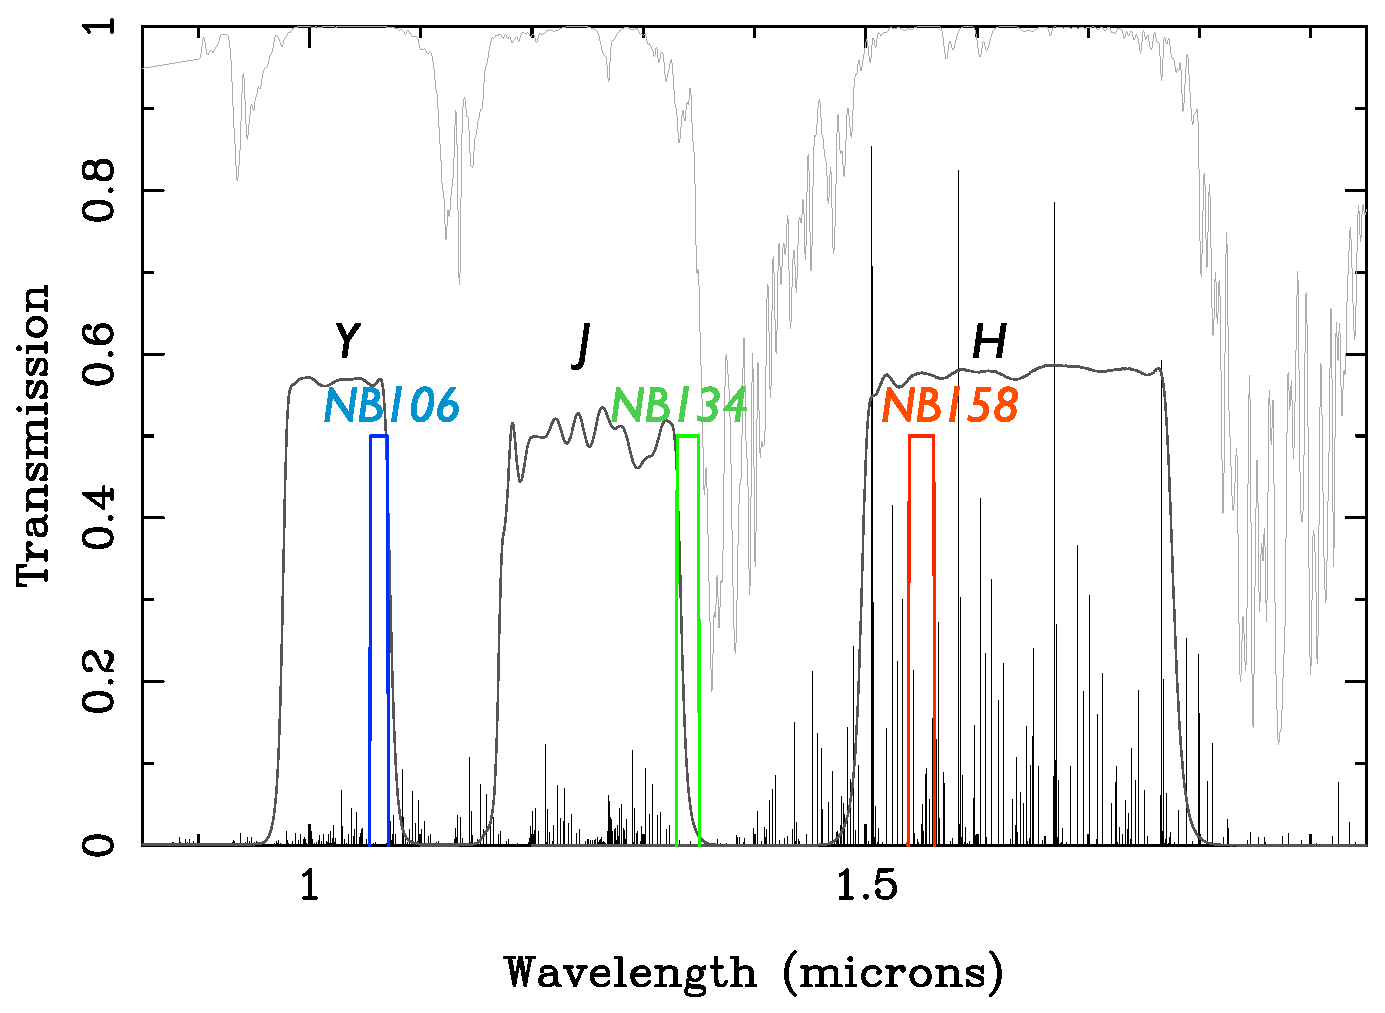
\includegraphics[width=80mm]{\thisdir figs/iwata_pg_filters_nbf01vd.eps}
}
\caption{
Transmission curves of NBFs considered. Transmission curves for $Y$,
 $J$, $H$-bands and the atomospheric transmission, and OH air glow
 strength (in arbitrary unit) are also shown.
}
\label{fig:iwata_filter_nbf}
\end{figure}

\par\noindent
[Very narrow band width filters]


\par\noindent
[What should be clarified with ULTIMATE-SUBARU.]

\subsection{Proposed Observations}

\par\noindent
[Target objects: sample selection, number of objects, number of observing
fields, sky area.]

\par\noindent
[Observing modes: imaging or spectroscopy.]

\par\noindent
[Required observing time:]

\par\noindent
[Special requirements for ULTIMATE-SUBARU other than baseline
specifications, if any.]

\subsection{Synergy and Competitions}

\subsubsection{Synergy with TMT}

\subsubsection{Competitions with other facilities}

Instruments for 8--10m class telescopes.

ELT instruments.

Space-based projects.

\bibliographystyle{apj}
\bibliography{\thisdir nbf}

\include{science/koyama/ykoyama}
\include{science/saito/saito}
\include{science/imanishi/ImanishiSJ}
\include{science/shibuya/shibuya}
\include{science/yasui/yasui}
\include{science/chiba/chiba}
\include{science/nishiyama/nishi}
\include{science/pyo/pyo}
\include{science/fukagawa/fukagawa}
\include{science/iwata/sci_summary} %\section{Science Summary: System Requirements}

%%% AO Simulation
%%%%%%%%%%%%%%%%%%%%%%%%%%%%%%%%%%%%%%%%%%%%%%%%%%%%%%%%%%%%%%%%%%%%%%%%%
% NGAO$B%o!<%/%7%g%C%WJs9p=q(B                                              %
%%%%%%%%%%%%%%%%%%%%%%%%%%%%%%%%%%%%%%%%%%%%%%%%%%%%%%%%%%%%%%%%%%%%%%%%%
%\documentclass[10pt]{jarticle}
%\usepackage{graphicx}

%\oddsidemargin   -0.25cm
%\evensidemargin  -0.25cm
%\topmargin       -0.25cm
%\textwidth        16.5cm
%\textheight       24.0cm
%\parindent        10pt

%%%%% OYA's personal new commands %%%%%
\newcommand %%%% \protect is necessary for captions %%%%%
{\supstar}{\!\!\mbox{\protect\raisebox{1.5ex}{$\star$}}}
\newcommand{\gtrsim}{\ ^{\displaystyle >}_{\displaystyle \sim}\ }
\newcommand{\lesssim}{\ ^{\displaystyle <}_{\displaystyle \sim}\ }
\newcommand{\adeg}{\hbox{$\,^{\circ}$}}
\newcommand{\arcs}{\hbox{$\,^{\prime\prime}$}}
\newcommand{\arcm}{\hbox{$\,^{\prime}$}}

\def\thisdir{simulation/glao/}

%\begin{document}

\chapter{Next-Generation AO Simulation Study
\label{chap:simulation}}

$BK\>O$G$O$9$P$kK>1s6@<!@$Be9-;kLnJd=~8w3X7O$N$?$a$N(B
$B%7%_%e%l!<%7%g%s$K4p$E$/8!F$7k2L$r$^$H$a$k!#(B
$BJd=~8w3XAuCV(B(AO: Adaptive Optics)$B$N;kLn$r9-$2$k$?$a$K$O!"(B
$BBg5$$f$i$.$N(B3$B<!859=B$$r9MN8$9$kI,MW$,$"$j!"$3$N5;=Q$r%H%b%0%i%U%#!<$H8F$V!#(B
$B%H%b%0%i%U%#!<5;=Q$r4QB,L\E*$K1~$8$F<BAu$9$k$3$K$J$k$,!"$=$NJ}<0$K$OJ#?t(B
$B$"$k(B(\ref{sec:various_ao_systems}$B@a;2>H(B)$B!#(B
$B$=$NCf$G(B
$BCOI=AXJd=~8w3X7O(B(GLAO: Ground-Layer Adaptive Optics)$B$H(B
$BB?E7BNJd=~8w3X7O(B(MOAO: Multi-Object Adaptive Optics)
$B$KBP$7$F%7%_%e%l!<%7%g%s$K$h$k8!F$$r9T$C$?!#(B

$B$9$P$kK>1s6@$K<!@$Be9-;kLn(BAO$B$rMQ$$$?@V30@~4QB,AuCV$,(B
$B3hLv$7;O$a$k:"$K$O!"8}7B(B30m$BK>1s6@$b;OF0$9$k$H4|BT$5$l$k!#(B
$B$9$P$kK>1s6@$N>-Mh7W2h$r9M$($k>e$G$O!"(B
$BL\;X$9%5%$%(%s%9$H$=$l$r<B8=$9$k5;=Q$H$$$&N>LL$K$*$$$F(B
30m$BK>1s6@$H$NAjJd@-$"$k$$$O(B30m$BK>1s6@$X$NH/E8$r0U<1$;$6$k$r$($J$$!#(B
GLAO$B$H(BMOAO$B$H$$$&(B2$B$D$N9-;kLn(BAO$B$NJ}<0$b$3$NMM$JGX7J$rF'$^$($F(B
$B%7%_%e%l!<%7%g%s$K$h$k8!F$$r?J$a$k8uJd$H$7$FA*Br$7$?!#(B
%
GLAO$B$O;kLnD>7B(B10$BJ,0J>e$H$$$&(B
$B9-;k(BAO$B$NCf$G$b:GBg$N;kLn$rC#@.$G$-$kJ}<0$G$"$k!#(B
$BJd@5@-G=$O2s@^8B3&$G$O$J$/%7!<%$%s%0$N2~A1$G$"$k$,!"(B
$B$3$N;kLn$r3h$+$9$3$H$G(B30m$BK>1s6@$HAjJdE*$J2J3XE*8&5f@.2L$,4|BT$G$-$k!#(B
$BFC$K%^%&%J!&%1%"$OBg5$$f$i$.A4BN$NCf$GCOI=AX$,@j$a$k3d9g$,Bg$-$$$3$H$,(B
$BCN$i$l$F$*$j(BGLAO$B$KE,$7$?%5%$%H$G$"$k$H8@$($k!#(B
%
MOAO$B$O9-$$;kLn$KOK$C$FF1;~$KJ#?t$NE7BN$r4QB,$9$k$3$H$G4QB,8zN($r(B
$B>e$2$k$3$H$,$G$-$kJ}<0$G$"$k!#3FE7BN$K$O2s@^8B3&$N6u4VJ,2rG=$,4|BT$G$-!"(B
$BLLJ,8w$H$NAj@-$bNI$$!#(B
MOAO$B$N<B8=$K$O?7$7$$5;=Q3+H/$,I,MW$G$"$k!#(B
$B0E$$4QB,E7BN$+$iN%$l$?J}8~$K$"$k==J,L@$k$$J#?t$NGHLL;2>H@1(B($B%,%$%I@1(B)$B$+$i!"(B
$B4QB,E7BNJ}8~$NGHLL$r?dDj$9$k%H%b%0%i%U%#!<5;=Q!"?dDj$5$l$?GHLL$r(B
$BGHLL%;%s%5(B(WFS)$B$,8+$F$$$J$$J}8~$N2DJQ7A6@(B(DM)$B$GJd@5$9$k%*!<%W%s%k!<%W@)8f5;=Q(B
$BEy$,5s$2$i$l$k!#(B
$B$9$P$kK>1s6@$K$*$$$F5;=QE*!"2J3XE*7P83$rC_@Q$7$F$$$/$3$H$G(B
30m$BK>1s6@$N<!4|4QB,AuCV$KH/E8$5$;$k$3$H$,4|BT$5$l$k!#(B

$B$3$3$G$N%7%_%e%l!<%7%g%s$O9-;kLn2=8!F$$N$?$a$G$"$k$N$G!"(B
$B$$$:$l$NJ}<0$KBP$7$F$b;kLn$r$I$3$^$G9-$/3NJ]$G$-$k$+$,(B
$B:G$b=EMW$J3NG'$9$Y$-E@$K$J$k!#(B
%
GLAO$B$N>l9g$OJd@5@-G=$,%7!<%$%s%0$K6a$$$N$G!"2s@^8B3&$r07$&0lHLE*$J(BAO$B$H$O(B
$B>u67$,0[$J$j%7!<%$%s%0$N1F6A$bBg$-$$!#(B
$B$3$N$h$&$JNN0h$G%7%_%e%l!<%7%g%s7k2L$,@5$7$$$+!"(B
$B$^$?%7!<%$%s%0%b%G%k$r$I$&Dj5A$9$k$+$KCm0U$,I,MW$G$"$k!#(B
%
MOAO$B$N>l9g$O!"8DJLE7BN$KBP$9$k9b%9%H%l!<%kHf$,L%NO$G$"$k$N$G(B
$B2s@^8B3&$N@-G=$r0];}$G$-$k;kLn$,$I$NDxEY$+!"$^$?$=$N$?$a$KI,MW$H$J$k(B
tip/tilt$B%,%$%I@1(B($BDc<!%,%$%I@1(B)$B$N?tEy$N>r7o$,CeL\$9$Y$-E@$G$"$k!#(B
%
$B$3$l$i$N9`L\$r%7%_%e%l!<%7%g%s$K$h$C$F3NG'$7$F$=$l$>$l$NJ}<0$N35MW$rGD0.$7$?(B
$B>e$G!"8!=P46EY$d%9%+%$%+%P%l!<%8$J$I$N$5$i$K>\:Y$J8!F$$X$HH/E8$5$;$F$$$/$3$H(B
$B$K$J$k!#(B

Sec.\ref{sec:gal_sim_imaging}$B$H(BSec.\ref{sec:spec_simulation}$B$G$O!"(B
GLAO$B%7%9%F%`$G$N1sJ}6d2O4QB,$,$I$N$h$&$J$b$N$K$J$k$+!"%J%A%e%i%k%7!<%$%s(B
$B%0$G$N4QB,$d2s@^8B3&$,C#@.$5$l$?>l9g$HHf3S$7$F8!F$$9$k!#(B
Sec.\ref{sec:gal_sim_imaging}$B$G$O;#A|4QB,$K$D$$$F!"(B
Sec.\ref{sec:spec_simulation}$B$G$OJ,8w4QB,$K$D$$$F$^$H$a$k!#(B



\clearpage
\begin{center}

\noindent
\Large
%%$BH/I=FbMF$N%?%$%H%k!JEvF|;H$C$?$b$N$HF10l$G$"$kI,MW$O$"$j$^$;$s!K(B
\section{Simulations of Subaru Next-Gen AO System: GLAO
\label{sec:glao_simulation}}
\vspace{0.5cm}

\noindent
\large
%%$BCx<T(B
{\bf Shin Oya$^1$}\\
$^1$ Subaru Telescope, 650 North Aohoku Place, Hilo, HI 96720, USA\\
\vspace{0.5cm}

\noindent
\normalsize
{\bf Abstract}
\end{center}
\vspace{-0.2cm}

\noindent
%abstract goes here...
$B$3$3$G$O9-;kLnJd=~8w3X7O$NCf$G$b(B10$BJ,3Q$rD6$($k:G$b9-$$;kLn$r3NJ]$G$-$k(B
$BCOI=AXJd=~8w3XAuCV(B(GLAO: Ground-Layer AO)$B$N8!F$7k2L$K4X$7$F5-=R$9$k!#(B
$B$3$NJ}<0$O>eAX$NBg5$$f$i$.$rJd@5$7$J$$$?$a!"2s@^8B3&$N@-G=$rF@$k$3$H(B
$B$G$O$J$/9-$$;kLn$K$o$?$C$F%7!<%$%s%0$r2~A1$9$k$3$H$rL\E*$H$7$F$$$k!#(B
GLAO$B$N<B8=J}K!$H$7$F$O2DJQI{6@$rF3F~$9$kJ}8~$G8!F$$r?J$a$F$$$k!#(B
$B2DJQI{6@$O(BGLAO$B0J30$K$b69;kLn$NE7BN$KBP$7$F9b$$%9%H%l!<%k$rC#@.$9$k(B
$B$3$H$,$G$-$k$N$G!"==J,L@$k$$C10l@1$KBP$9$k<+A3%,%$%I@1(B(NGS)$B4QB,!"(B
$B%3!<%s8z2L$rDc8:$9$k$?$a$NJ#?t%l!<%6!<%,%$%I@1(B(LGS)$B%H%b%0%i%U%#4QB,(B
$B$b9g$o$;8!F$$9$k$Y$-$@$H9M$($F$$$k!#(B
$B%7%_%e%l!<%7%g%s!&%3!<%I$O(BTMT$B$N(BNFIRAOS$B$N$?$a$K3+H/$5$l$?(BMAOS$B$r;HMQ$7$?!#(B



%%$BK\J83+;O!J>ON)$F$O<+M3!K(B

%%% 20130311 ommited by Iwata

%%%%%%%%%%%%%%%%%%%%%%%%%%%%%%%%%%%%%%%%%%%%%%%%%%%%%%%%%%%%%%%%%%%%%%%%%
%% NGAO$B%o!<%/%7%g%C%WJs9p=q%F%s%W%l!<%H(B
%%%%%%%%%%%%%%%%%%%%%%%%%%%%%%%%%%%%%%%%
%%
%% [AO$B$HAuCV$N;EMM(B] $B3F<+MW5a$9$k(BAO$B$dAuCV$N;EMM$r%F%s%W%l!<%H$K$"$kI=$K5-F~!#(B
%%
%% [$B;29MJ88%(B] $BI,$:L@5-$9$k$3$H!#?^$N0zMQ85$bL@5-$9$k$3$H!#(B
%%
%% [$BJ,NL(B] $B4pD49V1i(B(20$BJ,0J>e(B)$B$O(B4$B%Z!<%80J>e!"0lHL9V1i(B(15$BJ,(B)$B$O(B2$B%Z!<%80J>e!#(B
%%
%% [$BDy@Z(B] $B869FDy$a@Z$j(B 2012$BG/(B1$B7nKv(B
%%
%%%%%%%%%%%%%%%%%%%%%%%%%%%%%%%%%%%%%%%%%%%%%%%%%%%%%%%%%%%%%%%%%%%%%%%%%

%\documentclass[10pt]{jarticle}
%\usepackage{graphicx}

%\oddsidemargin   -0.25cm
%\evensidemargin  -0.25cm
%\topmargin       -0.25cm
%\textwidth        16.5cm
%\textheight       24.0cm
%\parindent        10pt

%\def\gsim{\mathrel{\raise0.35ex\hbox{$\scriptstyle >$}\kern-0.6em % Greater/squiggles
%\lower0.40ex\hbox{{$\scriptstyle \sim$}}}}
%\def\lsim{\mathrel{\raise0.35ex\hbox{$\scriptstyle <$}\kern-0.6em % Less than/squiggles 
%\lower0.40ex\hbox{{$\scriptstyle \sim$}}}}

%\begin{document}

\def\thisdir{simulation/moao/}

\begin{center}

\noindent
\Large
\section{Simulations of Subaru Next-Gen AO System: MOAO
\label{sec:moao_simulation}}
\vspace{0.5cm}

\noindent
\large
%%$BCx<T!JNc!K(B
{\bf Masayuki Akiyama$^1$}\\
$^1$ Astronomical Institute, Tohoku University, 3-6 Aramaki, Aoba-ku, Sendai, Japan
\vspace{0.5cm}

\noindent
\normalsize
{\bf Abstract}
\end{center}
\vspace{-0.2cm}

\noindent
$B$3$3$G$O$9$P$kK>1s6@$K$*$$$F(B6$B8D$N%l!<%6!<%,%$%I@1$rMQ$$$F(B
$BB?E7BNJd=~8w3X(B(MOAO)$B$r9T$C$?>l9g$KM=A[$5$l$k@-G=$r8!F$$7$?(B
$B7k2L$r$^$H$a$k!#FC$K!"(BMOAO$B$rMQ$$$k$3$H$GCO>eAXJd=~8w3X(B(GLAO)
$B$h$j$b9b$$Jd=~@-G=$r9-$$NN0h$NB?E7BN$K$D$$$F<B8=$9$k$3$H$r(B
$BL\;X$9!#$=$N$?$a(BGLAO$B$h$j$b9b$$Jd=~@-G=$r0];}$7$D$D!"$I$NDxEY(B
$B$^$G%?!<%2%C%HNN0h$r9-$2$i$l$k$N$+$rI>2A$9$k$3$H$K=EE@$r(B
$BCV$/!#(BMOAO$B$N>l9g$K$O;kLn$NCf$rO"B3E*$KJd@5$9$k$3$H$O$;$:!"(B
$BFCDj$N%?!<%2%C%H$NJ}8~$N$_$NJd@5$r9T$C$F$$$k$3$H$KCm0U$,(B
$BI,MW$G$"$k!#$=$N$?$a0J2<$G$O$3$N%?!<%2%C%H$rA*Br$9$kNN0h$N(B
$B$3$H$r%?!<%2%C%HNN0h$H8F$V!#(B6$B8D$N%l!<%6!<%,%$%I@1$rMQ$$$?(B
$B>l9g!"H>7B(B$3^{\prime}$$BDxEY$N%?!<%2%C%HNN0h$K$D$$$F$O(BGLAO
$B$h$j$b9b$$Jd=~@-G=$,4|BT$5$l$k$,!"$=$l$h$j$b%l!<%6!<%,%$%I@1$N(B
$B4V3V$r9-$2$F%?!<%2%C%HNN0h$r9-$2$k$H;kLn$N$[$H$s$I$NNN0h(B
$B$G(BGLAO$B$K6a$$Jd=~@-G=$7$+F@$i$l$:!"(BMOAO$B$N%a%j%C%H$,(B
$B@8$+$;$J$/$J$k$3$H$,$o$+$C$?!#$^$?<+A3%,%$%I@1$N4V3V$,3+$/$K$D$l(B
$B$F(B Tip-Tilt $B$NGHLL8m:9$,5^7c$KBg$-$/$J$k$3$H$b$o$+$C$?!#(B
Tip-Tilt $B%,%$%I@1$KMQ$$$k$3$H$N$G$-$k<+A3%,%$%I@1$NL@$k$5(B
$B$r9M$($k$H6d6KJ}8~$K$*$$$F$OJ#?t$N<+A3%,%$%I@1$r%?!<%2%C%H(B
$BNN0h$KMQ0U=PMh$k3NN($O$+$J$jDc$/!"(BTip-Tilt $B$NGHLL;D:9$,(B
$B@-G=$r%j%_%C%H$9$k!#(B


%%$BK\J83+;O!J>ON)$F$O<+M3!K(B

%%% 20130311 ommitted by Iwata

\include{science/minowa/minowa}
\include{science/iwata/ngao_spec_simulation}

%%% System Design
%\documentclass[10pt]{jarticle}
%\usepackage{graphicx}
%\usepackage{url}

%\oddsidemargin   -0.25cm
%\evensidemargin  -0.25cm
%\topmargin       -0.25cm
%\textwidth        16.5cm
%\textheight       24.0cm
%\parindent        10pt

%\def\gsim{\mathrel{\raise0.35ex\hbox{$\scriptstyle >$}\kern-0.6em % Greater/squiggles
%\lower0.40ex\hbox{{$\scriptstyle \sim$}}}}
%\def\lsim{\mathrel{\raise0.35ex\hbox{$\scriptstyle <$}\kern-0.6em % Less than/squiggles 
%\lower0.40ex\hbox{{$\scriptstyle \sim$}}}}

\def\thisdir{development/design/}

%\begin{document}

\chapter{System Study for Subaru Next-Generation AO
\label{chap:system_design}}

\section{Comparisons of Candidate AO Systems for Subaru Telescope
 Next-Generation AO
\label{sec:various_ao_systems}}

%%% 20130311 ommited by Iwata

\section{Overview of the System}

%%% 20130311 ommited by Iwata.
%%% Need to include overview of NIR instrument(s) as well?

$B8=;~E@$G5DO@$,?J$a$i$l$F$$$k<!@$Be(BAO$B$*$h$S@V30@~AuCV$N(B
$B4pK\;EMM$rI=(B\ref{tab:spec}$B$K<($7$?!#$3$N;EMM$O:#8e$N>\:Y$J(B
$B8!F$$K$h$C$F$OBgI}$KJQ99$5$l$k2DG=@-$,$"$k!#(B
\begin{table}[t]
\begin{center}
\begin{tabular}{|l|l|l|l|l|}
\hline
 Item & Specification \\
 \hline
 $B4QB,GHD90h(B & 0.9--2.5 $\mu$m ($B%5%$%(%s%9(BWS$B$+$i$NMW5a$O(B0.6--5$\mu$m\\
 $B4QB,%b!<%I(B & $B;#A|!"J,8w!JLLJ,8w$r9MN8$9$k!K(B\\
 $B4QB,;kLn(B & $\phi$ 15$BJ,3Q!J(B20$BJ,3QL\I8!K(B\\
 $B>GE@0LCV(B & $B%+%;%0%l%s>GE@(B \\
 \hline
 $B%,%$%I@1(B & 4 LGS$B!"(BNGS$B!J(B2$\sim$4$B8D$+!)!K(B\\
 $B%,%$%I@1$NA*BrHO0O(B & LGS$B$O4QB,;kLn$NC<!"(BNGS$B$O4QB,;kLnFb(B \\
 $BGHLL%;%s%5!<(B & $B%,%$%I@1$K$=$l$>$l(B1$B$D$:$D(B (Guide star oriented)\\
 $BGHLL%;%s%5!<%?%$%W(B & $B%7%c%C%/%O%k%H%^%s7?!J%T%i%_%C%I7?$bMW8!F$!K(B \\ 
 $BGHLL%;%s%5!<AG;R?t(B & 100$BDxEY$+$=$l0J>e(B ($B9b%9%H%l!<%k$J$i(B1000$BAG;RDxEY$b(B) \\
 $BGHLL%;%s%5!<%5%s%W%j%s%0<~GH?t(B & 500Hz$B0J>e!J(BGLAO$B$O(B100Hz$B$G$b2D!K(B \\
 $B2DJQ7A6@(B & $BI{6@$r2DJQ7A6@2=(B \\
 $B2DJQ7A6@AG;R?t(B & 500$\sim$1000$BDxEY(B \\
 $BGHLL@)8f%b!<%I(B & GLAO (LTAO$B!"(BExAO$B$J$I$X$N@ZBXBP1~$,I,MW$+!)(B)\\
 \hline
\end{tabular}
\caption{$B<!@$Be(BAO$B$*$h$SAuCV$N4pK\;EMM0F(B}
\label{tab:spec}
\end{center}
\end{table}

\section{Technical Challenges}

$B>e=R$7$?(BTomography AO$B$K6&DL$9$k5;=QE*$J2]Bj$O!"(B
$B%l!<%6!<5;=Q$*$h$SJ#?t%l!<%6!<%,%$%I@1$N@=:n5;=Q!"(B
$BBg5$$f$i$.$N9b$5J}8~$N(Btomography$B?dDj5;=Q!"(B
$B2DJQI{6@!"@)8f7W;;5!$J$I$,$"$k!#(B
$B$?$@$7!"@$3&$ND,N.$H$7$F(Btomography AO$B$O@9$s$K(B
$B%7%9%F%`8!F$!"5;=Q8!F$$,?J$a$i$l$F$*$j!"(B
$B5;=QE*$J2]Bj$O$+$J$j9nI~$5$l$D$D$"$k$N$,8=>u$G$"$k!#(B

$B=i4|$N%l!<%6!<%,%$%I@1$O?'AG%l!<%6!<$,<gBN$G$"$C$?!#(B
$B$3$l$O%l!<%6!<G^<A$,1UBN$G$"$j!"0BDj@-!"J]<i@-$K(B
$BBg$-$JO+NO$,I,MW$G$"$k!#$^$??'AG$NNt2=$K$h$k=PNODc2<$,(B
$BHr$1$i$l$J$$!#<!$KH>F3BN%l!<%6!<$H%l!<%6!<7k>=$N(B
$B5;=QH/E8$,$"$j!"8GBN%l!<%6!<$,BfF,$7$F$/$k!#(B
$B:#$G$O%J%H%j%&%`AX$rNe5/$9$k$?$a$NOB<~GHH/@8$rMQ$$$?(B
$BA48GBN%l!<%6!<$,5;=QE*$K@.=O$7$F$-$?!#(B
Gemini$B$N(BMCAO$B$G$O=PNO(B50W$B$N%l!<%6!<$r(B5$B$D$KJ,3d$7$F!"(B
5$B8D$N%J%H%j%&%`%l!<%6!<%,%$%I@1$N:n@.$K@.8y$7$F$$$k!#(B
$B0lJ}!"%U%!%$%P!<%l!<%6!<5;=Q$rMQ$$$?%3%s%Q%/%H$+$D(B
$B0BDj$7$?%l!<%6!<$N3+H/$,(BESO$B$rCf?4$K?J$a$i$l!"(B
$B%I%$%D$N(BTOPTICA$B<R$H%+%J%@$N(BMPB$B<R$N6&F1$G(B
$BO"B3GH(B20W$B$N%l!<%6!<$,@=IJ2=$5$l$?!#(B
$B$3$N%l!<%6!<$OB>$N(B8m$B%/%i%9$N<!@$Be(BAO$B$*$h$S(B
ELT$BMQ(BAO$B$N%l!<%6!<%,%$%I@1MQ8w8;8uJd$H$7$FBg$-$J(B
$B4|BT$,4s$;$i$l$F$$$k!#2f!9$b$9$G$K(BMPB$B<R$H(B
$BHkL)J];}7@Ls$rDy7k$7!"5;=Q>pJs$N8r49!"(B
$B4pK\;EMM$N8!F$=`Hw$r?J$a$F$$$k!#(B
$B$^$?!"%l%$%j!<;6Mp$rMxMQ$7$?%l!<%6!<%,%$%I@1$b(B
WHT$B!"(BMMT$B$J$I$GCOF;$K;n83$,B3$1$i$l$F$$$k!#(B
8m$B%/%i%9$N(Bsingle conjugate $B%l!<%6!<%,%$%I@1(BAO$B$,(B
$B0BDj$7$F1?MQ$5$l$F$*$j!"%l!<%6!<%,%$%I@1$K(B
$B4X$9$k4pAC5;=Q!"1?MQ5;=Q$O$*$*$$$K?JJb$7$?!#(B
$B%l!<%6!<%7%9%F%`$K$D$$$FI=(B\ref{tab:Laser}$B$K$^$H$a$?!#(B

\begin{table}[t]
\begin{center}
\begin{tabular}{|l|l|l|l|l|l|l|l|}
\hline
 %$BK>1s6@(B & Subaru & Keck I & Keck II & Gemini N & VLT  & Gemini S & LBT \\
% \hline
%$B%l!<%6!<%,%$%I@1(B & Na$BAX(B & Na$BAX(B & Na$BAX(B & Na$BAX(B. & Na$BAX(B  & Na$BAX(B & $B%l%$%j!<;6Mp(B \\
%$B%l!<%6!<%?%$%W(B & $BOB<~GH(B & $BOB<~GH(B & $B?'AG(B & $BOB<~GH(B. & $B?'AG(B->$B%U%!%$%P!<(B  & $BOB<~GH(B & $BA48GBN%0%j!<%s(B \\
%$B%l!<%6!<G^<A(B & $B8GBN7k>=(B & $B8GBN7k>=(B & $B?'AGM-5!1UBN(B & $B8GBN7k>=(B. & $B?'AGM-5!1UBN(B->$B8w%U%!%$%P!<(B  & $B8GBN7k>=(B & $B8GBN7k>=(B \\
%$B=PNO(B & $\sim$6W & $\sim$40W & $\sim$15W & $\sim$15W & $\sim$10W->$\sim$25W & $\sim$10W / beacon & $\sim$18W / beacon \\
%$B%l!<%6!<H/?67ABV(B & 143MHz & 75MHz & 13kHz or 26kHz & 75MHz & $BO"B3GH(B & 75MHz & 10kHz \\
$B%,%$%I@1%?%$%W(B & \multicolumn{3}{|c|}{$B%J%H%j%&%`AX(BLGS} &  \multicolumn{1}{|c|}{$B%l%$%j!<(BLGS} \\
\hline
$B%l!<%6!<%?%$%W(B & $B?'AG(B & $BA48GBNOB<~GH(B & $B8w%U%!%$%P!<%l!<%6!<(B & $BA48GBN!!(B\\
\hline
$B%l!<%6!<G^<A(B & $B1UBNM-5!MOG^(B & $B8GBN7k>=(B & $B8w%U%!%$%P!<(B& $B8GBN7k>=(B \\
\hline
$BK>1s6@(B & Keck II & Subaru, Keck I & VLT$B!J<!@$Be!K(B & LBT \\
             & VLT & Gemini N\&S &       &  (Na-LGS$B$b7W2hCf(B) \\
\hline
$B=PNO(B & 15W(Keck II) & 6W(Subaru) & 25W(VLT$B<!@$Be(B) & 18W$\times$3 (LBT) \\
    &    &  40W(Keck I) & & \\
    &  10W(VLT) & 15W(GeminiN) & &  \\
    &    &  10W$\times$5 (GeminiS) & & \\
\hline
$BH/?67ABV(B & 26kHz(Keck II) & 143MHz(Subaru) & $BO"B3GH(B(VLT$B<!@$Be(B) & 10kHz(LBT) \\
  & $BO"B3GH(B(VLT) & 75MHz(Keck I) & & \\
  &   & 75MHz(Gemini N\&S) & & \\
\hline
\end{tabular}
\caption{$B%l!<%6!<%,%$%I@1MQ%l!<%6!<%7%9%F%`$NHf3S(B}
\label{tab:Laser}
\end{center}
\end{table}


$B:GBg3QEY$G$b(B10$BJ,3Q$H$$$&69$$HO0O$N8w8;$rMQ$$$F!"(B
$BESCf$K$"$kBg5$$f$i$.$N(B3$B<!85J,I[$r?dDj$9$k(B
tomography$B?dDj5;=Q$O!"0lHL$N(B3$B<!85(Btomography$B$H$O(B
$B$+$J$j0[$J$kMWAG$r4^$s$G$$$k!#$7$+$7!"B?$/$N(B
AO tomography$B%"%k%4%j%:%`$,Ds>'$5$l!"7W;;5!(B
$B%7%_%e%l!<%7%g%s!"%F%9%H%Y%C%I$K$h$k<B83$,(B
$B?J$a$i$l$F$-$?!#>\:Y$J8!F$$*$h$S%7%9%F%`$KFC2=$7$?(B
$B8!F$$O$^$@I,MW$G$"$k$,!"4pACE*$J(BAO tomography$B$N(B
$B8&5f$O==J,$J$5$l$F$-$F$$$k!#$9$P$k<!@$Be(BAO$B8!F$(B
$B%o!<%-%s%0%0%k!<%W$O!":#8e>\:Y8!F$$rB3$1$F$$$/M=Dj$G$"$k!#(B

$BFC$K(BGLAO$B$O2DJQI{6@$,=EMW$J%3%s%]!<%M%s%H$H$J$k!#(B
$BF|K\$G$O$^$@2DJQI{6@$N8!F$$O?J$a$i$l$F$$$J$$$,!"(B
$B%"%j%>%J$N(BMMT$B!"(BLBT$B$G$O$9$G$K2DJQI{6@$,Ek:\$5$l!"(B
$BL@$k$$%,%$%I@1$G$h$$Jd@5@-G=$rC#@.$7$F$$$k!#(B
$B$^$?%A%j$N(BVLT$B$N$?$a$N2DJQI{6@$,@=:nCf$G$"$k!#(B
$B$3$l$i$N2DJQI{6@$r@=:n$7$?$N$O%$%?%j%"$N(BMicrogate$B<R$G$"$k!#(B
$B2f!9%o!<%-%s%0%0%k!<%W$O$9$G$K(BMicrogate$B<R$H%3%s%?%/%H$r$H$j!"(B
$B$9$P$kK>1s6@MQ$N2DJQI{6@$N35G08!F$$N=`Hw$r?J$a$F$$$k!#(B

$BJ#?t$N%,%$%I@1!"J#?t$"$k$$$OB?AG;R$N2DJQ7A6@$r@)8f$9$k$?$a$N(B
$B7W;;5!$KMW5a$5$l$k@-G=$OHs>o$K9b$$!#2f!9%o!<%-%s%0%0%k!<%W$O!"(B
$B$^$@@)8f7W;;5!$N8!F$$r;O$a$F$$$J$$$,!"(BTMT$BMQ$N%U%!!<%9%H%i%$%H(BAO
$B$G$"$k(BNFIRAOS$B$N@)8f7W;;5!8!F$$,==J,;29M$K$J$k$H9M$($F$$$k!#(B

\section{Interfaces with the Subaru Telescope -- 20130311Iwata: to be ommitted?}

$B$9$P$kK>1s6@<!@$Be(BAO$B$NBh0l8uJd$G$"$k(BGLAO$B$K$D$$$F!"(B
$BK>1s6@$H$N%$%s%?!<%U%'!<%9$r9M;!$7$?!#(B
GLAO$B$N:GBg$NFCD'$O!"2DJQI{6@$rMQ$$$F$$$k$3$H$G!"(B
$BH?<MLL$,>/$J$/8zN($,9b$$$3$H$,$"$2$i$l$k!#(B
$B=>$C$F!"4QB,AuCV$O%+%;%0%l%s>GE@$K@_CV$9$k$N$,$h$$!#(B
$B$^$?!"(BGLAO$B$G$O(B10$BJ,3Q$rD6$($k;kLn$,L%NO$H$J$C$F$$$k!#(B
$B8=:_;H$o$l$F$$$k%+%;%0%l%s>GE@$N2D;kMQBg5$J,;6Jd@58w3X7O$O(B
$B$=$3$^$G$N;kLn$r3NJ]$G$-$F$$$J$$!#(BGLAO$B$H6a@V30@~4QB,AuCV$N(B
$BAH$_9g$o$;$N$H$-$OBg5$J,;6Jd@58w3X7O$O<h$j30$9I,MW$,$"$k!#(B

$B%+%;%0%l%s>GE@$N4QB,AuCV$N8!F$$b=EMW$G$"$k!#(B
GLAO$B$N9-;kLn$r@8$+$96a@V30@~;#A|J,8wAuCV$r8!F$$9$k>e$G!"(B
$BK>1s6@$N8w3X<}:9!"AuCV$N%5%$%:!"=ENL!"@_7W@=B$2DG=$J8w3X7O$N@_7W(B
$B$J$I$,=EMW$J%U%!%/%?!<$H$J$k!#(B

$B2DJQI{6@$O$9$P$kK>1s6@$N%H%C%W%f%K%C%H$K@\B3$5$l$k!#(B
$B$9$P$kK>1s6@$O<g>GE@It$K9-;kLn%+%a%i$J$I$r(B
$BEk:\$9$k$?$a!"%H%C%W%f%K%C%H8r495!$N=ENL@)8B$,(B
3t$B$G$"$k!#8=:_@=:nCf$N(BVLT$BMQ2DJQI{6@$NAm=ENL$O(B1500kg
$BDxEY$J$N$G7ZNL2=$NEXNO$OITMW$G$"$k!#(B
$B8=:_;HMQCf$N@V30I{6@$OD>7B$,(B1265mm$B$G$"$j!"(B
VLT$B$N2DJQI{6@D>7B$h$j$b<c43Bg$-$$!#(B
$B%+%;%0%l%s>GE@$N(BF$BCM$NJQ99$b9MN8$7$?2DJQI{6@$N;EMM:vDj$r(B
$B:#8e?J$a$F$$$/$3$H$K$J$k!#(B
$B%H%C%W%f%K%C%H$K$*$1$kEENO6!5k!"@)8f@~!"%M%C%H%o!<%/!"Nd5Q?e(B
$B$J$I$N4pK\E*$J%$%s%U%i!"%H%C%W%f%K%C%H$H$N%$%s%?!<%U%'!<%9!"(B
$B$J$I$N8!F$$b=EMW2]Bj$G$"$k!#(B

\section{Subaru GLAO System Structure}


%%% 20130311 ommitted by Iwata

%%% 20130311 additions by Iwata
\section{Components of GLAO: Adaptive Secondary Mirror}

\section{Components of GLAO: Wavefront Sensing System}

\section{Components of GLAO: Laser System}

\section{Components of GLAO: RTC}

%%% 20130311 additions by Iwata
\section{Telescope Modifications}

\subsection{Top Unit}

\subsection{Cassegrain Focus}

\subsection{Other Areas?}



\section{Operations of GLAO}

$B$9$P$kK>1s6@$O<g>GE@4QB,AuCV$,$"$k$?$a!"2DJQI{6@$r>o@_$9$k$3$H$O(B
$B1?MQ>e$G$-$J$$!#$=$N$?$a!"2DJQI{6@$O%H%C%W%f%K%C%H8r49AuCV$r(B
$BMQ$$$FCeC&$9$kI,MW$,$"$k!#$=$N$?$a$N%$%s%?!<%U%'!<%9;EMM$r(B
$B3NDj$7$J$1$l$P$J$i$J$$!#$^$?2DJQI{6@$NIT;HMQ;~$NJ]4I>l=j$N3NJ]$H(B
$B$=$N%$%s%?!<%U%'!<%9$H%$%s%U%i$N;EMM$K$D$$$F$b7h$a$kI,MW$,$"$k!#(B
$B$^$?!"8r49;~$N4D6->r7o!"?6F0>r7o!"6@$NJ];}$"$k$$$O0BA4$J>uBV4IM}$K(B
$B$D$$$F$b8!F$$rMW$9$k!#(B

$B0lJ}!"$9$P$kK>1s6@$NI{6@$OFLLL$G$"$k!#FLLL$N2DJQI{6@$N%-%c%j%V%l!<%7%g%s(B
$BJ}K!$K$D$$$F$b8!F$$,I,MW$@!#$^$?!"2DJQI{6@$N:F>xCe$NI,MW@-!"Dj4|E*$J(B
$BJ]<i9`L\$J$I$b=i4|8!F$$NCJ3,$G5DO@$7$F$*$/$Y$-$G$"$m$&!#(B

$B%l!<%6!<<M=P%7%9%F%`$O!"K>1s6@$N%;%s%?!<%;%/%7%g%s$K>o@_$9$k$3$H$r(B
$B8!F$Cf$G$"$k!#CeC&$NI,MW@-$O$J$$$,!"%l!<%6!<$NJ]<i!"ItIJ$N8r49!"(B
$B7PG/JQ2=$X$NBP1~!"0BA44IM}$r4^$a$?%l!<%6!<1?MQBN@)$OI,?\$H$J$k!#(B

$BGHLL%;%s%5!<$O%+%;%0%l%s>GE@>eIt$N%+%;%0%l%s%U%i%s%8$H8F$P$l$kCf$K(B
$B@_CV$5$l$k!#$3$NItJ,$O%"%/%;%9$,BgJQFq$7$/!"AuCV$N8N>c!"2~=$$,(B
$BFq$7$$!#$=$N$?$a$N7xO4!"J]<iITMW$NGHLL%;%s%5!<%7%9%F%`8!F$$OBg@Z$G$"$m$&!#(B

\section{Perspective of Future Development}

GLAO$B%7%9%F%`$O<g$H$7$F2DJQI{6@!"%+%;%0%l%s%U%i%s%8$NGHLL%;%s%5!<!"%l!<%6!<(B
$B<M=P7O!"4QB,AuCV$H$$$&9=@.$+$i$J$k!#$3$N%3%s%]!<%M%s%H$OB>$N(BAO$B%7%9%F%`$K(B
$B$H$C$F$b=EMW$J9=@.MWAG$G$"$k!#(B

$B2DJQI{6@$NAG;R?t$O(B1000$BDxEY$H$J$k8+9~$_$G$"$k!#$=$N$?$a!"L@$k$$<+A3%,%$%I@1MQ$N(B
$BGHLL%;%s%5!<$r4QB,AuCVB&$KMQ0U$9$k$H!"%+%;%0%l%s!"%J%9%_%9$N$$$:$l$N>GE@$K$b(B
Extreme AO$BAuCV$,$G$-$k!#$b$A$m$s!"8=B8$"$k$$$O7W2hCf$N9b%3%s%H%i%9%H4QB,AuCV$K$b(B
$B1~MQ$,$G$-$k$G$"$m$&!#2DJQI{6@$OCf4V@V30@~$NAuCV$NGX7J8w$r2!$5$($kMxE@$H$b$J$k!#(B

$B$^$?!"J#?t%l!<%6!<<M=P7O$O(BMOAO$B$KMxMQ$G$-!"2DJQI{6@$O(BMOAO$B$N(Bwoofer$B$H$7$F;HMQ$7!"(B
$B4QB,AuCVB&$K(BMOAO$B$N(Btweeter$B2DJQ7A6@$r$b$?$;$k$3$H$G!"8zN($NNI$$AuCV$,9M0F$G$-$k$G$"$m$&!#(B

$B$3$N$h$&$K(BGLAO$B%7%9%F%`$OK>1s6@5!G=$N%]%F%s%7%c%k$NDl>e$2$r$9$k$b$N$G$"$k!#(B

%\end{document}


%%% Instruments
%\chapter{Instruments for Subaru Next-Generation AO}
\def\thisdir{instrument/}

\chapter{Instruments for Subaru Next-Generation AO
\label{chap:inst}}


\section{Requirements on Instrument from Scientific Objectives}

Here we re-summarize the requirements from key science cases on
instrument specifications.

\begin{itemize}
 \item Field of view
 \item Pixel scale
 \item Requirements on broad-band filters (numbers, wavelength coverages)
 \item Requirements on narrow-band filters (numbers, spectral resolution,
      wavelength uniformity, wavelength coverages)
 \item Spectroscopy: Spectral resolution 
 \item Requirements on multi-object spectrograph mode
\end{itemize}

In this chapter we summarize the studies we have made so far on
instruments for ULTIMATE-SUBARU.

\def\thisdir{instrument/optics/}

\begin{center}
\section{Studies of the Optics for the Wide-Field Near-IR Imager and
 Multi-object Spectrograph
\label{sec:inst_optics}}
\vspace{0.5cm}

\noindent
\large
%% authors
{\bf T. Yamamuro$^{1}$, K. Motohara$^{2}$, I. Iwata$^{3}$ and Subaru
Telescope Next-Gen AO Instrument sub-working group}\\
$^1$ Optocraft
$^2$ Institute of Astronomy, University of Tokyo
$^3$ Subaru Telescope, National Astronomical Observatory of Japan
\vspace{0.5cm}

\end{center}

Here we summarize results of studies made by Dr. Yamamuro (Optcraft).
Document Number: CP0046--11--RP001 (w/o FoV split), CP0046--12--RP001 (w
FoV split).

\subsection{Optical Design without FoV Split}

First we studied how wide field of view can be achieved at the
Cassegrain focus of Subaru Telescope with the following conditions:

\begin{itemize}
 \item Single set of optics can be used (i.e., no FoV split is
       considered).
 \item We consider a near-infrared camera and spectrograph. Wavelength
       range is from 0.8$\mu$m to 2.5$\mu$m. The optics will be cooled
       down to about 100K.
 \item The target image quality is to achieve FWHM $<0.15''$ over the
       entire FoV in all of $J$, $H$, $K$-bands.
 \item The focal plane of the instrument should be flat so that we can
       achieve the above image quality by using science detectors with
       flat pixel arrays.
 \item The use of Teledyne H4RG (15$\mu$m pixel size) is assumed.
 \item The sizes of optical components should be feasibile; for example,
       the maximum size of components made of CaF$_2$ and BaF$_2$ should
       be less than 40cm.
\end{itemize}

We examined the two cases on the telescope parameters; (A) the case we
use the existing optical parameters of Subaru Telescope and (B) the case
with new parameters for the secondary mirror and also that the shape of 
primary mirror can be adjusted within the range of the stroke which the
existing mirror actuators are achievable.

Also, we should consider the necessity of field flatner for the
telescope focus. In order to achieve multi-object spectroscopy (MOS), we
need to insert a mask with slitlets at the telescope focus. Since the
Cassegrain focal plane has a curvature, in order to enable the use of
flat MOS mask, we need to insert field flatning lens(es). For the case
A, we show both the case with and without field flatner.

\subsubsection{A. Cases in which Subaru Telescope optical parameters are
   not changed}

Here we show the simplest case where there is no change in the telescope 
parameters and no field flatner is included.
Fig.\ref{fig:optcraft_fig01} is the optical layout. It consists of nine
collimator lenses and seven camera lenses. Lense materials are CaF$_2$, 
BaF$_2$, Fused silica, and ZnSe.The last lens of the camera section is
aspherical. 

\begin{figure}[!ht]
\centerline{
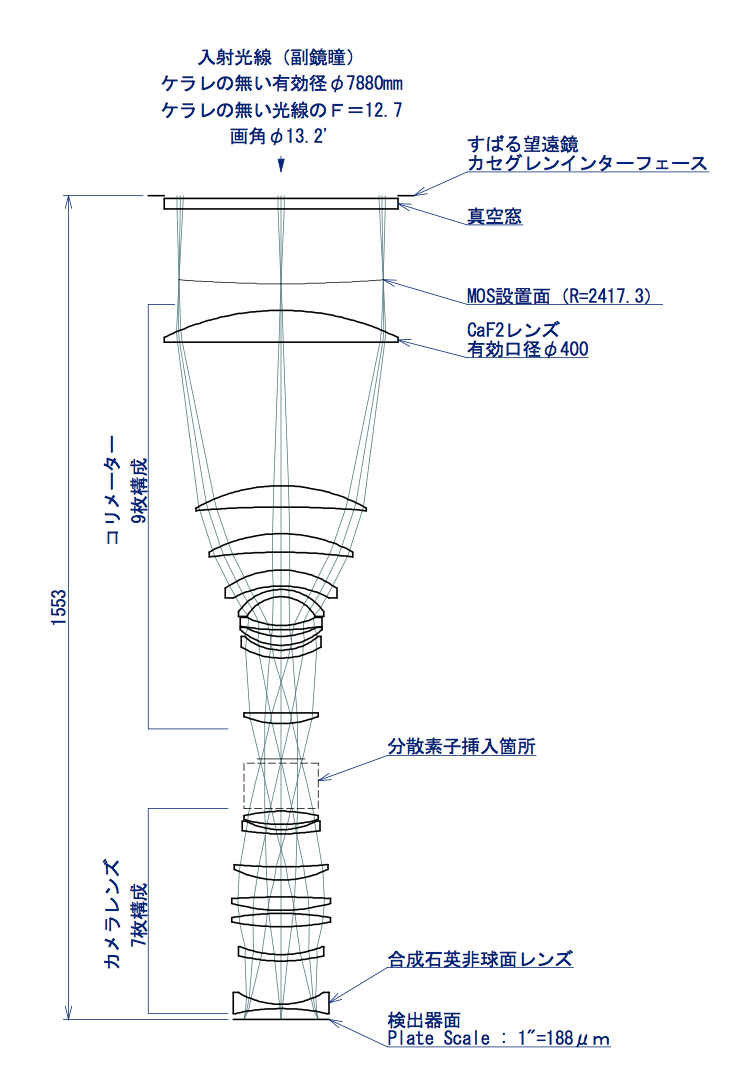
\includegraphics[width=120mm]{\thisdir figs/optcraft_fig01.eps}
}
\caption{Optical layout for Case A: no change in the telescope
 parameters. The case without field flatner.
}
\label{fig:optcraft_fig01}
\end{figure}

The field of view is determined so that the size of effective beam for
the largest lens is within $\phi$400mm, and in this solution it is 
$\phi 13.2'$. The effective diameter of the primary mirror is 
$\phi 7.88$m to achieve the above FoV at the secondary mirror pupil and
to block the light outside of the primary mirror (physical size 
$\phi$8.2m). Since this layout does not include field flatner, the
telescope focal plane has a curvature, and there is astigmatism.

The spot diagram at the position of the MOS mask (with a radius of
curvature of 2417.3mm) is shown in
Fig.~\ref{fig:optcraft_fig02}(left). The degradation of the image toward
the edge of FoV ($\sim 0.2''$ at the edge) is due to astigmatism. 
In this case the slit width at the edge should be adjusted to this image
quality. 
Fig.~\ref{fig:optcraft_fig02}(right) shows the size of distortion at the
position of the MOS mask.

\begin{figure}[!ht]
\centerline{
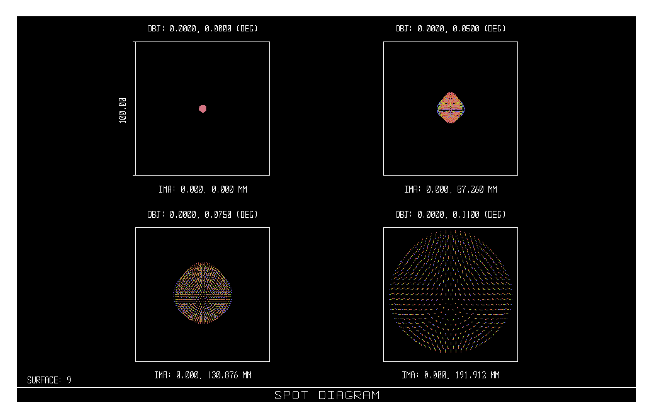
\includegraphics[width=100mm]{\thisdir figs/optcraft_fig02.eps}
 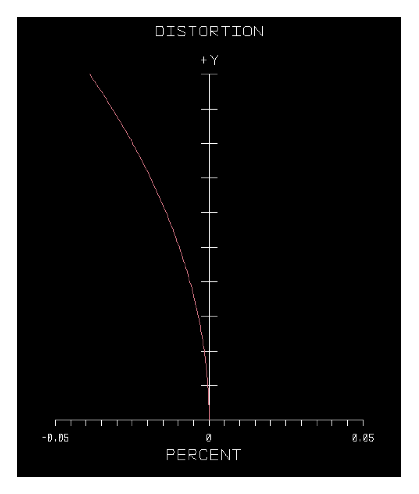
\includegraphics[width=60mm]{\thisdir figs/optcraft_fig03.eps}
}
\caption{(Left) Spot diagram at the position of the MOS mask with a
 curvature radius of 2417.3mm for a configuration shown in 
Fig.\ref{fig:optcraft_fig01}. Spot diagrams with wavelengths from
 0.8$\mu$m to 2.5$\mu$m are shown altogether, as wavelength dependence
 is small. (Right) distortion at the
 position of the MOS mask. The value is $-0.04$\% at the edge.
}
\label{fig:optcraft_fig02}
\end{figure}

The spot diagram and distortion at the position of the detectors are
shown in Fig. \ref{fig:optcraft_fig04}. All FWHM values are smaller than
the target FWHM (0.15$''$) except the case with 0.8$\mu$m
at the edge ($6.6'$) in which the FWHM is slightly larger than
0.15$''$. However, the distortion is large; at the edge it is 
$-6.3$\%.

\begin{figure}[!ht]
\centerline{
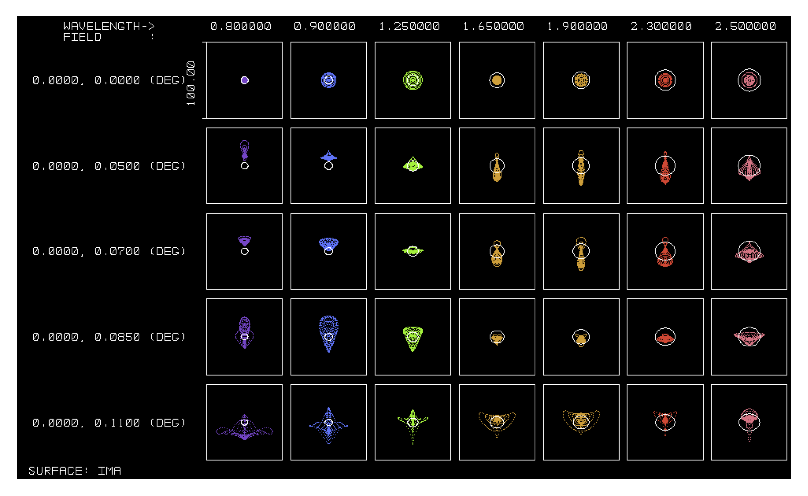
\includegraphics[width=120mm]{\thisdir figs/optcraft_fig04.eps}
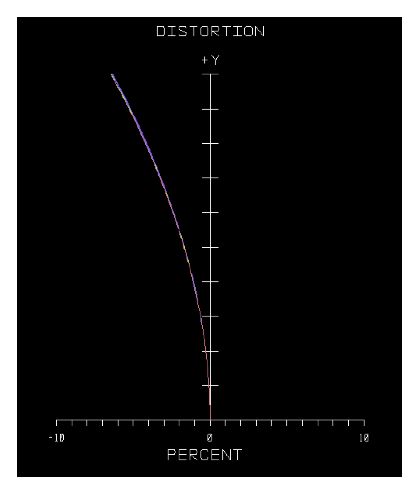
\includegraphics[width=60mm]{\thisdir figs/optcraft_fig05.eps}
}
\caption{(Left) Spot diagram at the position of the detectors for a
 configuration shown in Fig.\ref{fig:optcraft_fig01}.
Five positions from 0$'$ (center) to 6.6$'$ (edge) are shown along the
 vertical axis, and the cases with wavelengths from 0.8$\mu$m to
 2.5$\mu$m are plotted along the horizontal axis. 
The box size is 100$\mu$m which corresponds to 0.53$''$.
(Right) Distortion at the position of the detectors.
}
\label{fig:optcraft_fig04}
\end{figure}


We also evaluated the performance in spectroscopy. As a preliminary
analysis, here we only examined the image quality in spectroscopy in the
range 0.8--2.5$\mu$m without order-sorting.
Fig.~\ref{fig:optcraft_fig06} shows the positions of images in
spectroscopy as a function of wavelength.
Here we assume a fused silica grism with 160 grooves/mm, blaze angle 
34$\circ$\footnote{In section ** we examine more details of various
grisms}.
Fig.~\ref{fig:optcraft_fig07} is the spot diagram. Image qualities at
the shorter and longer wavelength edges and at the edge of FoV is not
good; in 2.5$\mu$m and at $6.6'$ from the center the RMS spot diameter
is $0.22''$. However, it is $0.17''$ at $5.5'$ from the center, and
at the other positions the image quality meets the goal.

\begin{figure}[!ht]
\centerline{
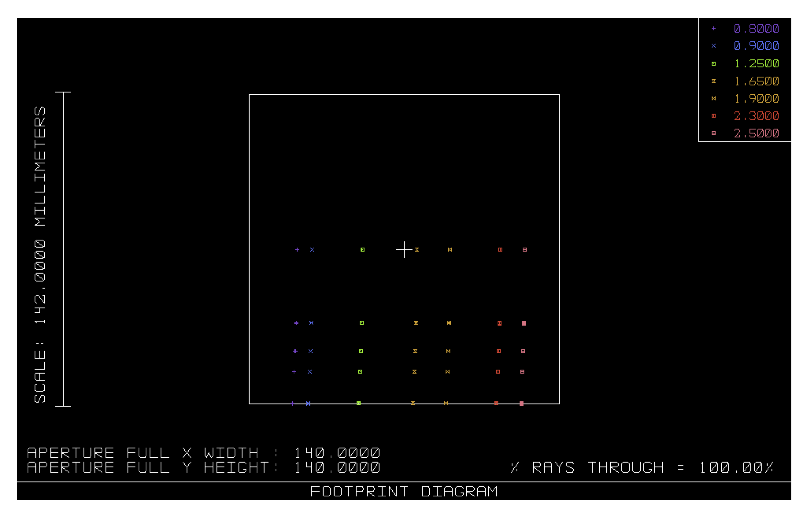
\includegraphics[width=120mm]{\thisdir figs/optcraft_fig06.eps}
}
\caption{Spectroscopic image positions for a configuration shown in Fig.~\ref{fig:optcraft_fig01}.
}
\label{fig:optcraft_fig06}
\end{figure}

\begin{figure}[!ht]
\centerline{
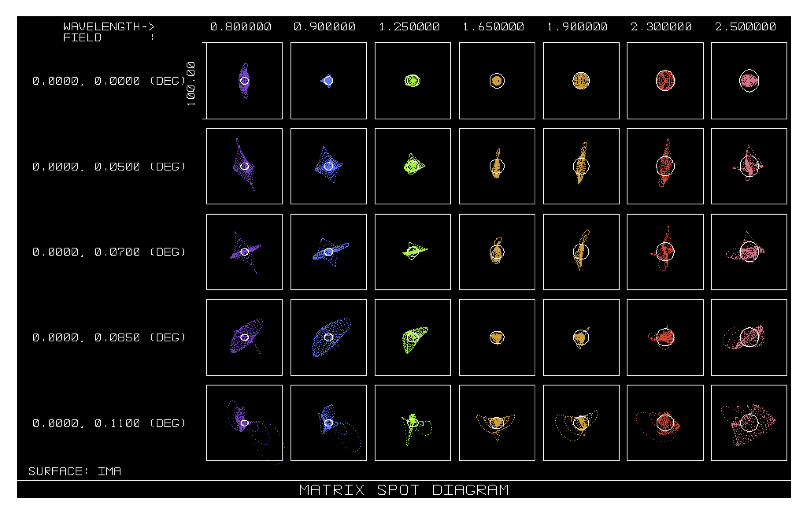
\includegraphics[width=120mm]{\thisdir figs/optcraft_fig07.eps}
}
\caption{Spot diagram for spectroscopy with a configuration shown in
 Fig.~\ref{fig:optcraft_fig01}.}
\label{fig:optcraft_fig07}
\end{figure}

Next we examined the case where there is no change in the telescope
parameters again, and a field flatner which consists of two lenses. 
Fig.~\ref{fig:optcraft_fig08} shows the optical layout of the case.

\begin{figure}[!ht]
\centerline{
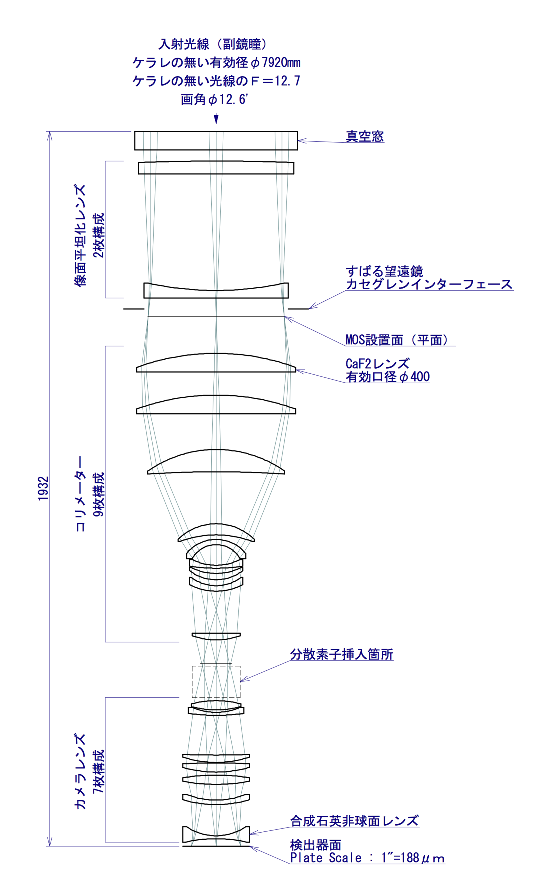
\includegraphics[width=120mm]{\thisdir figs/optcraft_fig08.eps}
}
\caption{Optical layout for Case A: no change in the telescope
 parameters. The case with field flatner.
}
\label{fig:optcraft_fig08}
\end{figure}

The optical design was made so that the effective diameter of the
largest lens is no larger than $\phi$400mm, as it is in the case without
the flatner. The field of view is $\phi 12.6'$, which is slightly
smaller than the case without the flatner, because the field flatner
acts like a concave lens and we need collimator lenses larger than the
flatner. The effective diameter of the primary mirror to block the light
outside of the primary mirror is $\phi$7.92m.
In addition to make the telescope focal plane flat, the addition of the
flatner enables a correction of astigmatism. As shown in 
Fig.~\ref{fig:optcraft_fig09}, the image quality is good at the flat MOS
mask, and there is no chromatic abberation.
We should note that there is distortion, which amounts +0.73\% at the
edge of the FoV.

\begin{figure}[!ht]
\centerline{
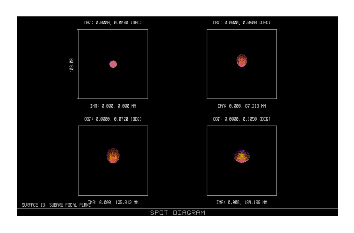
\includegraphics[width=100mm]{\thisdir figs/optcraft_fig09.eps}
 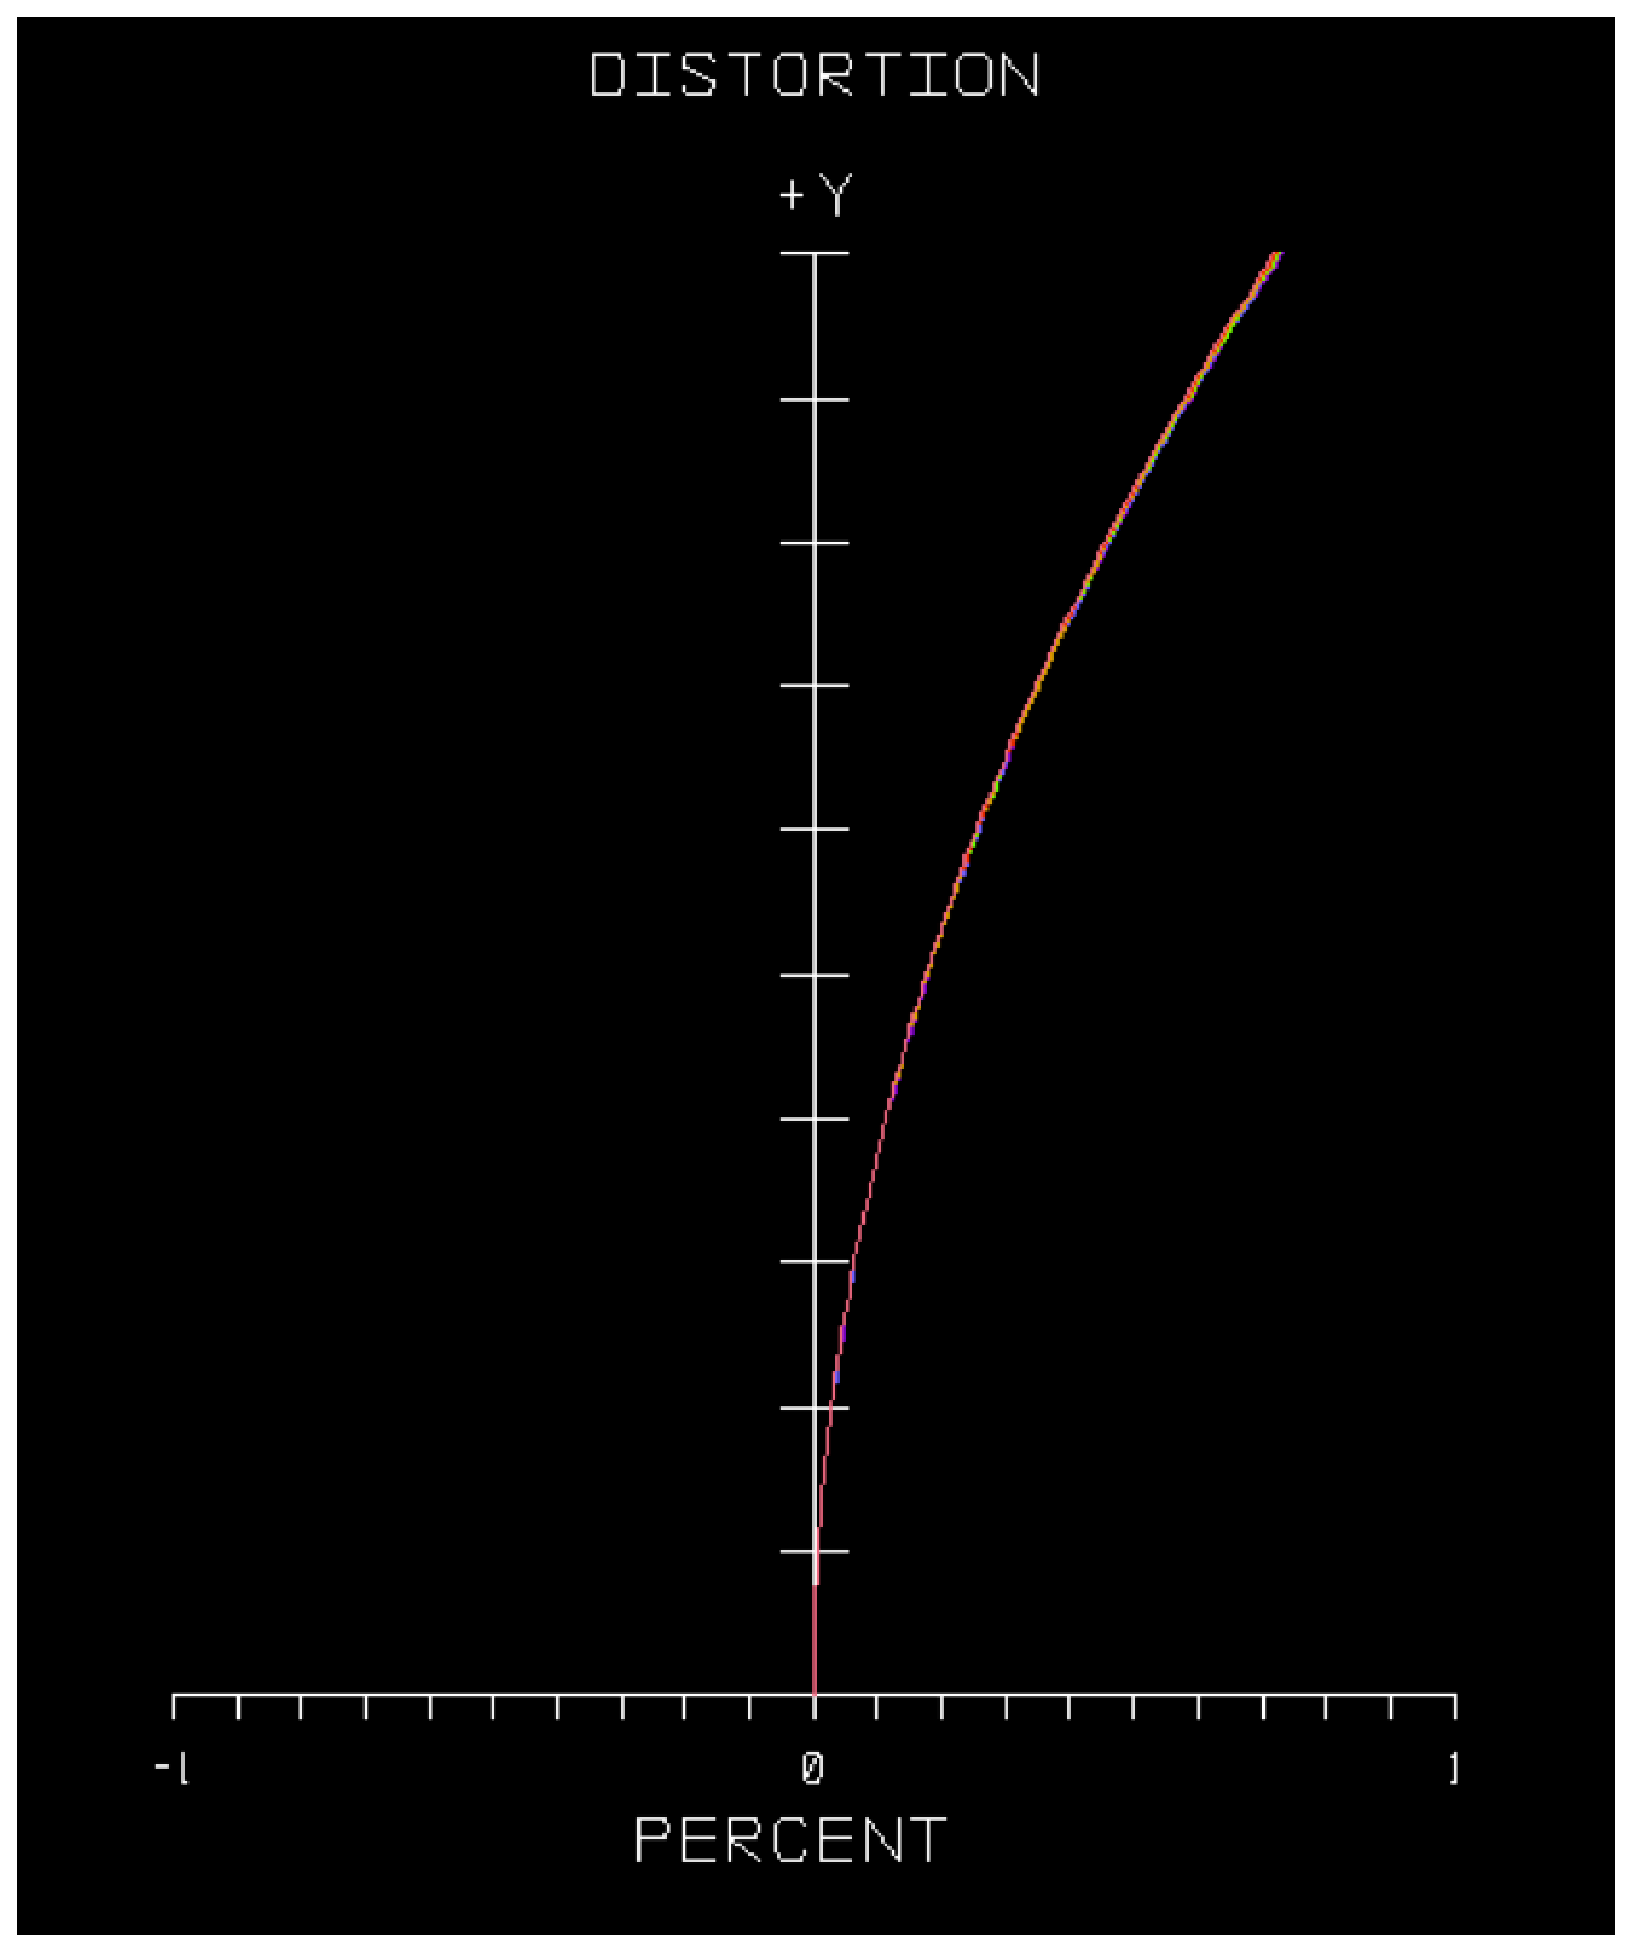
\includegraphics[width=60mm]{\thisdir figs/optcraft_fig10.eps}
}
\caption{(Left) Spot diagram at the MOS mask plate.
(Right) distortion at the MOS mask plate.
}
\label{fig:optcraft_fig09}
\end{figure}

For the image quality at the position of the detectors, similar to the
case without the flatner, in the most of the FoV and for the most of the
wavelength range the image quality satisfies the goal (FWHM smaller than
approx. $0.15''$), while in a few cases (such at the FoV edge ($6.3'$
from the center) and with 0.8$\mu$m) the image quality is slightly worse
than the goal. Distortion is large; it is $-5.2$\% at the edge of FoV.
Performance in the spectroscopy is also similar to the case without the
flatner, and in most cases the qulality satisfies the goal.
We should note that with the field flatner the optical layout is not
telecentric, and the plate scale should be changed if there is a focus
offset.  So the focusing is more important in this case.




\subsubsection{B. Cases in which Subaru Telescope optical parameters are
   changed}

Next we examined the case in which Subaru Telescope's optical parameters
are changed. In order to make the telescope's F number smaller, the
primary mirror's aspheric parameters should be negative. The actuator
storoke for the primary mirror is guaranteed up to 12$\mu$m. We assume
the conic parameters so that displacement at the edge of the primary
mirror is 12$\mu$m, and set F number to be 9.8.

The parameters of the secondary mirror is determined as it is optimal
for this Cassegrain wide-field instrument, and it is independent from
the existing secondary mirrors of Subaru Telescope.
It is a bipolar mirror with a diameter of $\phi$1544mm. The radius of
curvature is 7233.308mm and the conic constant is $-2.35464$.
The field of view is determined by the effective maximum size of the
lens ($\phi$400mm), and it is $\phi16.2'$.
Thanks to the smaller F number, the field of view is 28\% larger than
the case without changing the telescope parameters. The effective
diameter of the primary mirror to avoid the beam outside of the
secondary pupil and primary mirror ($\phi$8.2m) is $\phi$7.93m.

\begin{figure}[!ht]
\centerline{
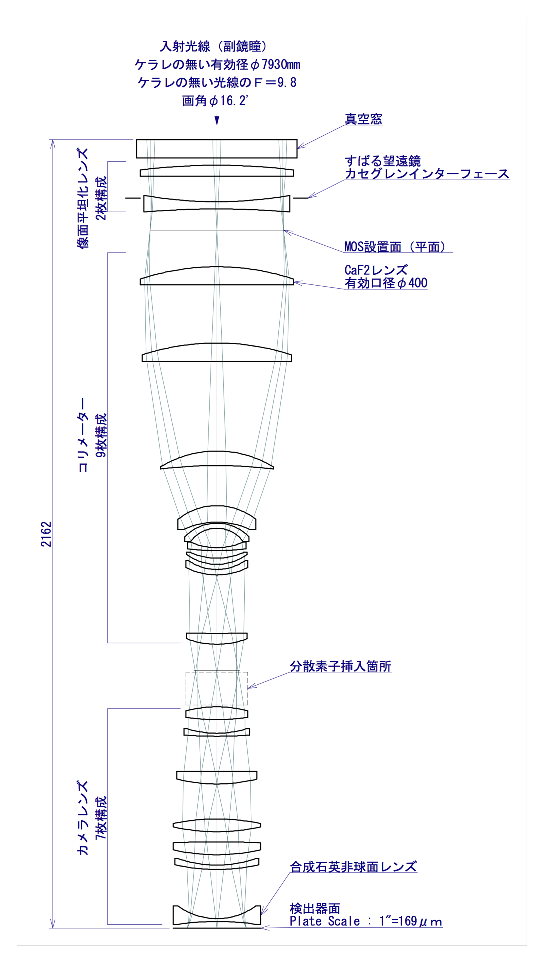
\includegraphics[width=120mm]{\thisdir figs/optcraft_fig15.eps}
}
\caption{The optical layout of the case B: Subaru Telescope
 optical parameters are modified. A field flatner is included in this
 design. 
}
\label{fig:optcraft_fig15}
\end{figure}

In this design a set of lenses as a field flatner is included. 
The spot diagram at the flat MOS mask position is presented in 
Fig. \ref{fig:optcraft_fig16}.
Although small coma aberration is present, its effect is small. There is
no chromatic aberration, overall image quality is good, although there
is distortion aberration at the edge of the FoV.

\begin{figure}[!ht]
\centerline{
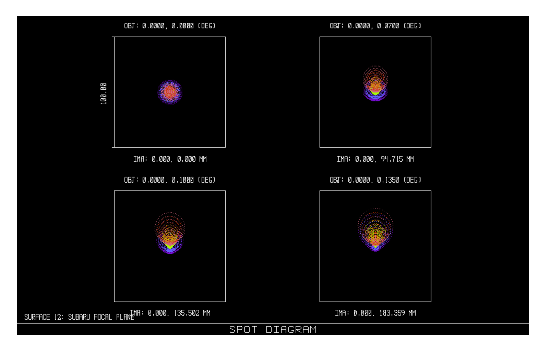
\includegraphics[width=100mm]{\thisdir figs/optcraft_fig16.eps}
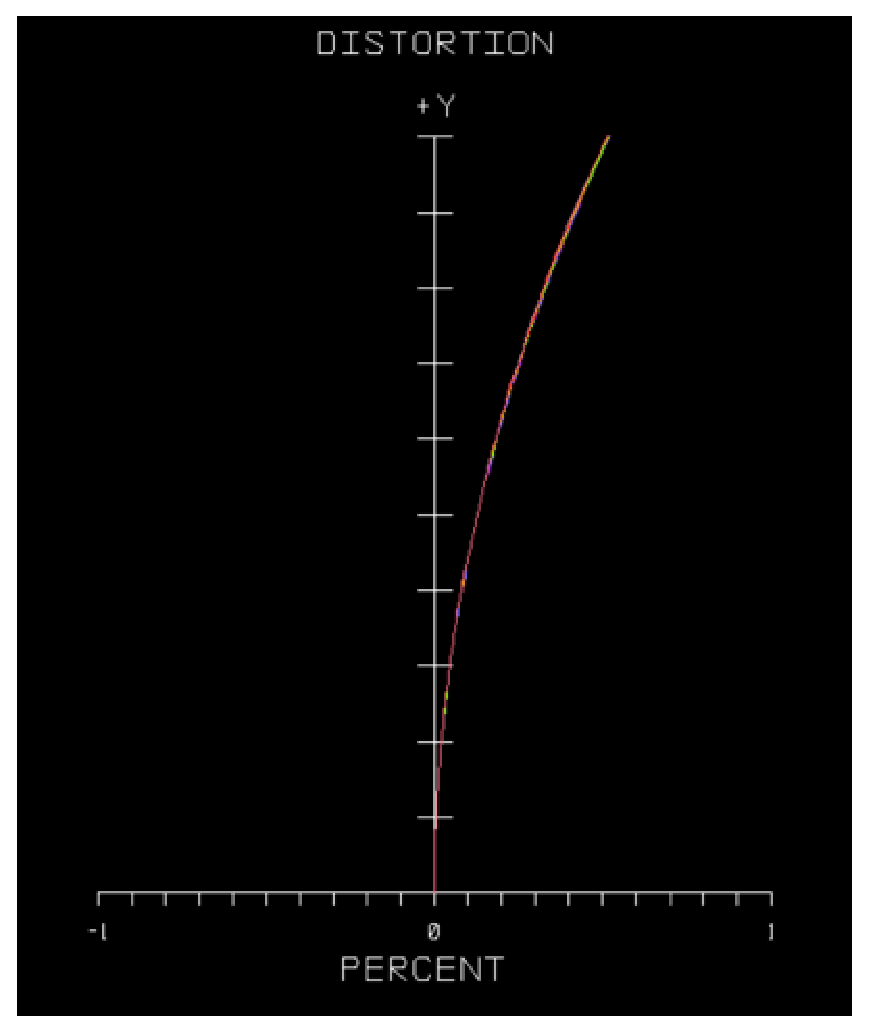
\includegraphics[width=60mm]{\thisdir figs/optcraft_fig17.eps}
}
\caption{(Left) Spot diagram at the MOS mask position.
(Right) distortion aberration at the MOS mask position.
}
\label{fig:optcraft_fig16}
\end{figure}

The configuration of optics after MOS position is similar to the case
without change of the telescope parameters: collimator with nine lenses
and camera with seven lenses. The focal plane is flat. The optical
layout in shown in Fig.\ref{fig:optcraft_fig15}.

In Fig. \ref{fig:optcraft_fig18} we show the spot diagram and distortion
aberration at the position of detectors.
Image quality at outskirt of the FoV ($>6'$) in a short wavelength
(0.8--0.9$\mu$m) degrades by $\sim0.2''$. Otherwise image quality
satisfies the goal (FWHM$\sim 0.15''$).
The maximum distortion aberration at the edge of FoV is $-1.24$\%, which
is smaller than the cases without changes in telescope parameters.

\begin{figure}[!ht]
\centerline{
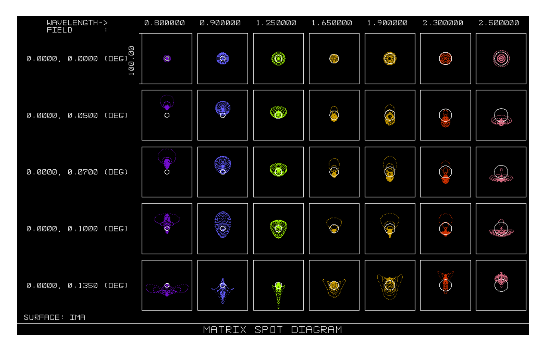
\includegraphics[width=120mm]{\thisdir figs/optcraft_fig18.eps}
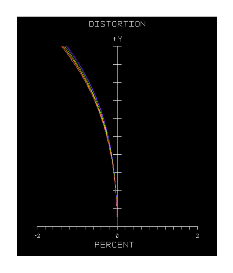
\includegraphics[width=60mm]{\thisdir figs/optcraft_fig19.eps}
}
\caption{(Left) Spot diagram at the positions of the detectors.
Images with five positions within the FoV (vertical) and seven
 wavelengths from 0.8$\mu$m to 2.5$\mu$m (horizontal) are plotted.
The box size is 100$\mu$m, which corresponds to $0.59''$.
The RMS spot diameters are $0.2''$ (at $8.1'$, $0.8\mu$m), 
$0.16''$ (at $6'$, $0.8\mu$m), $0.19''$ (at $6'$, $0.9\mu$m), and for
 other positions and wavelength the spot diameters are within $0.15''$.
(Right) Distortion aberration. It reaches to $-1.24$\% at the edge of
 the FoV.
}
\label{fig:optcraft_fig18}
\end{figure}

Performance in spectroscopy mode is examined and is reported in 
Fig.~\ref{fig:optcraft_fig20}. Here a grism made of fused silica, 160
lines/mm, blaze angle 35$^\circ$ is assumed, and the sizes of spectra on
the detector is presented.

In regards to the image quality, as shown in
Fig.~\ref{fig:optcraft_fig21}, in some cases at the edge of FoV or
shortest/longest wavelengths the RMS spot diameter becomes as large as 
$0.23''$. Otherwise the image quality satisfies the goal, especially
within $6'$ from the center of FoV.

\begin{figure}[!ht]
\centerline{
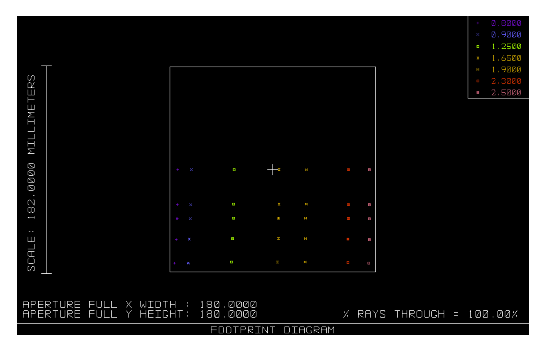
\includegraphics[width=120mm]{\thisdir figs/optcraft_fig20.eps}
}
\caption{
Spectroscopic image positions for a configuration shown in
 Fig.~\ref{fig:optcraft_fig15}. The box size is 180mm. We assume to use
 a grism made of fused silica with 160 lines/mm, and blaze angle
 35$^\circ$.
}
\label{fig:optcraft_fig20}
\end{figure}

\begin{figure}[!ht]
\centerline{
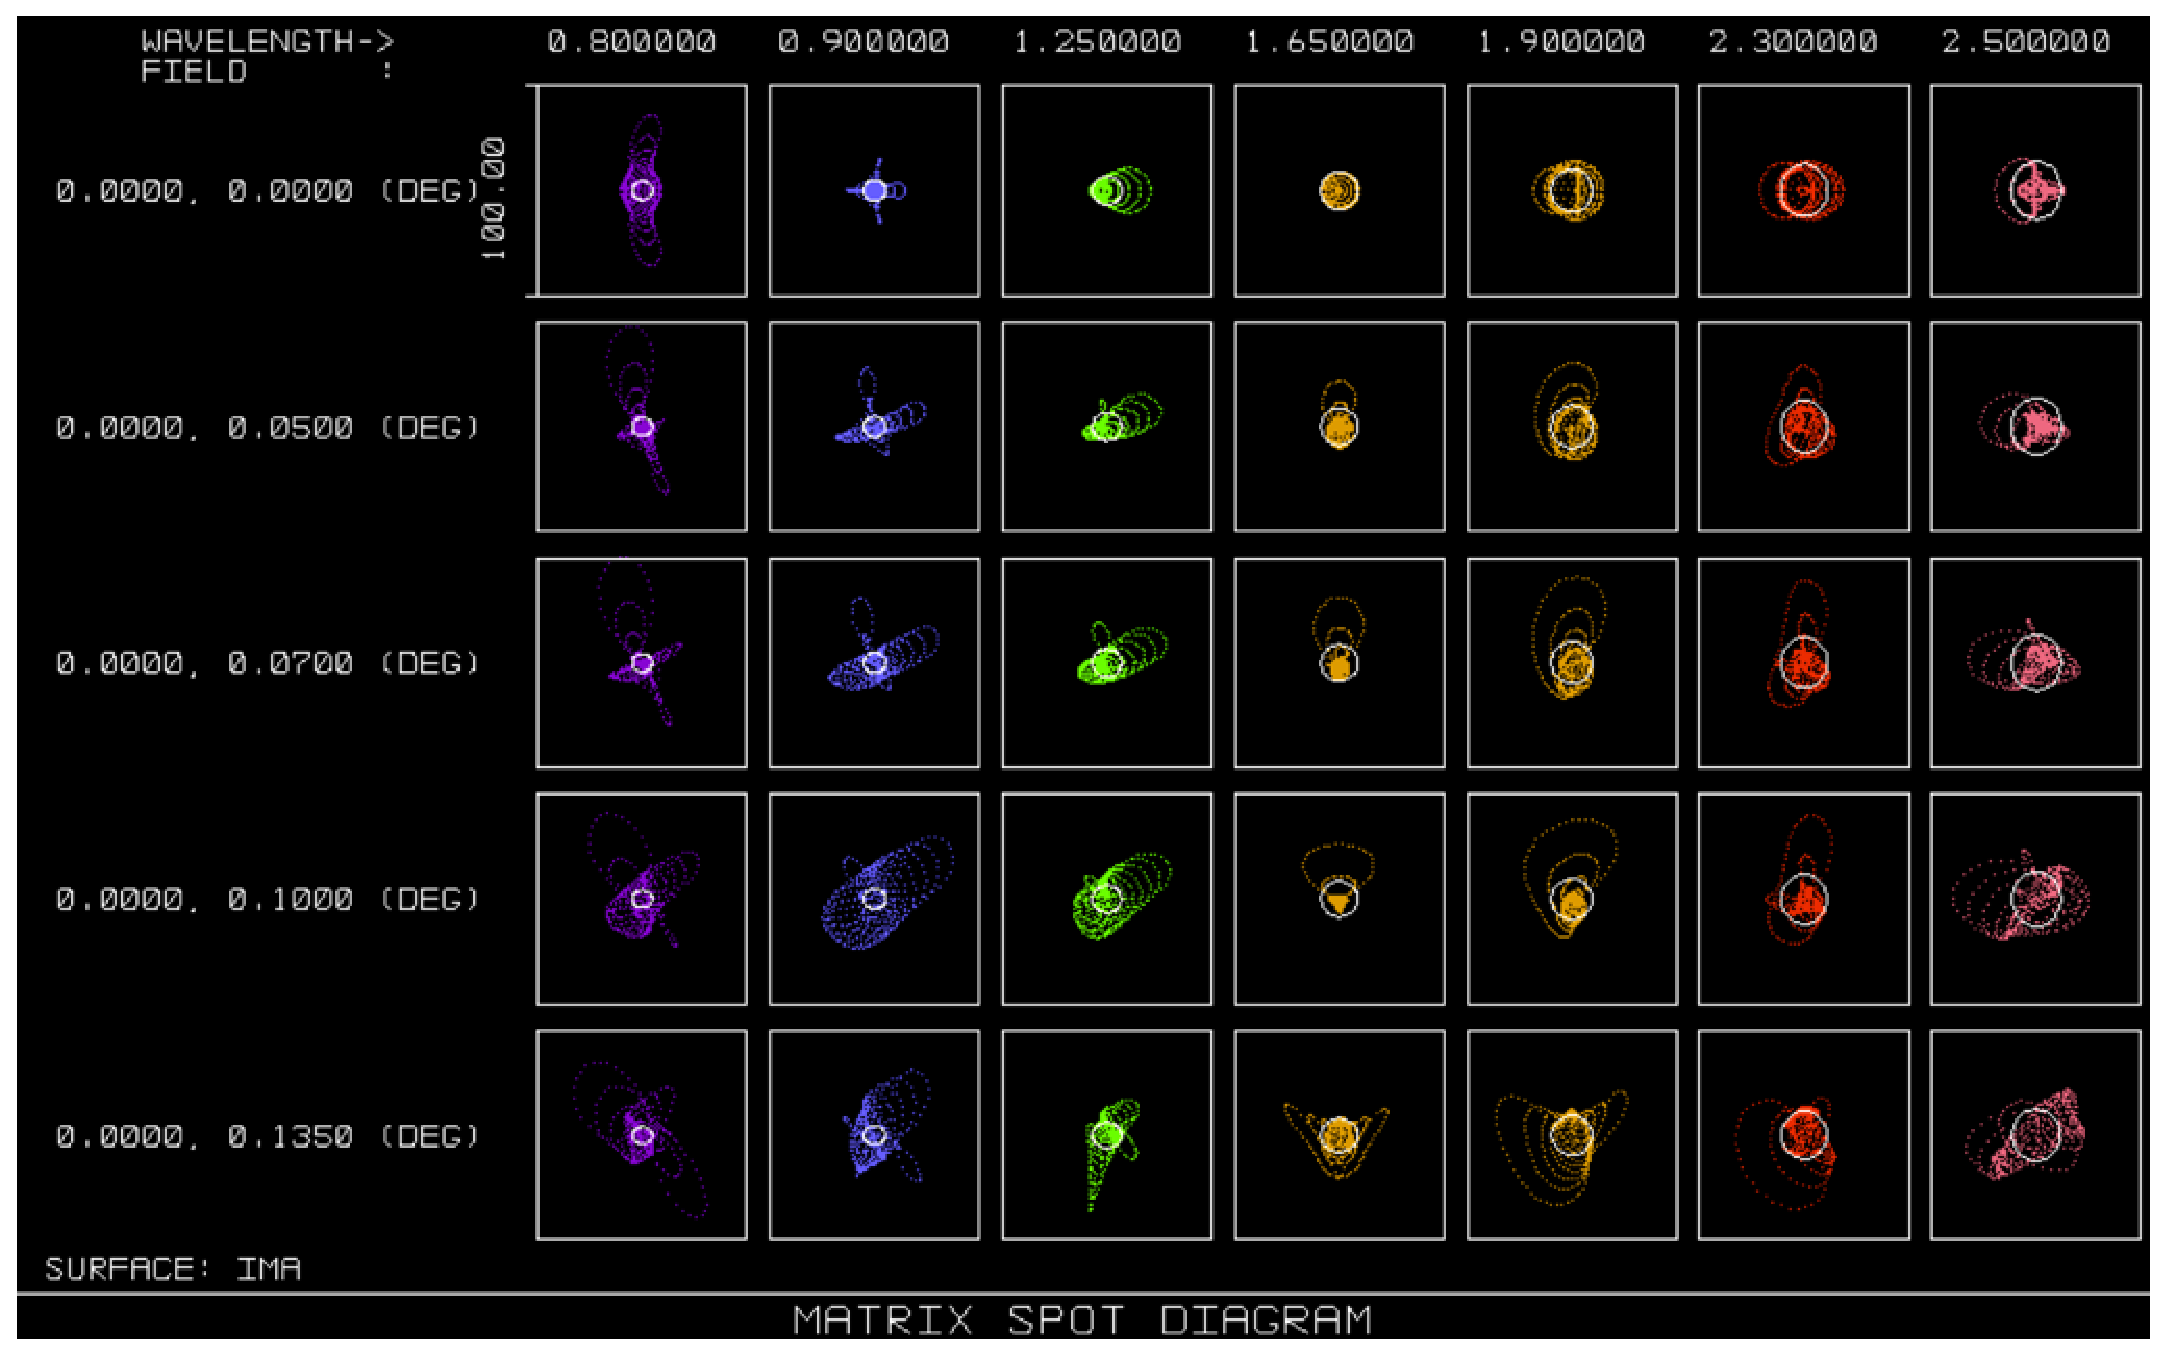
\includegraphics[width=120mm]{\thisdir figs/optcraft_fig21.eps}
}
\caption{Spot diagram for Case B, spectroscopy mode.
In shorter wavelength the performance is somewhat worse than the goal;
 at 0.8$\mu$m RMS spot diameters are in general 0.17--0.18$''$, and 
 0.2$''$ at 0.9$\mu$m. In longer wavelength spot diameter becomes larger
 at positions with distance from the center larger than $6'$ with
 $\lambda = 2.3-2.5\mu$m. Otherwise the image quality satisfies the goal
 ($0.15''$).
}
\label{fig:optcraft_fig21}
\end{figure}



\subsection{Optical Design with FoV Split}

\subsubsection{Case A: secondary mirror parameter is the same as
   existing one}

\subsubsection{Case B: secondary mirror parameter is modified}



%%% 20130906 iwata

\section{Optical Design Concept of Wide-field Imager for GLAO}

Proposed by J. Pazder (NRC-NSI-AST / HIA)

\bigskip

\section{Multi Integral-Field-Unit Instrument}

Describe overview of KMOS, discuss feasibility of Multi-IFU instrument
at the Cassegrain focus.

\bigskip

\section{Technical Issues of Wide-field NIR instrument}

\subsection{Mask Exchange Mechanism for MOS}

\subsection{Narrow-band Filters}

\subsection{Size and weight}


%%% Development Plan
\include{project/hayano/development_plan}

\include{project/actions/action_items}

\end{document}
